\documentclass[12pt,twoside,titlepage]{report}

%%%%%%%%%%%%%%%%%%%%%%%%%%%%%% Paquetes %%%%%%%%%%%%%%%%%%%%%%%%%%%%%%%%%%%%%

\usepackage[a4paper,bindingoffset=3mm,bottom=35mm]{geometry}
\usepackage[colorlinks=true,pdftex]{hyperref}   %%% Opcional. Para incluir marcadores y enlaces en el pdf
\usepackage[pdftex]{graphicx}  %%% para pdflatex. Las figuras pueden estar en pdf, jpg, svg y otros formatos
\usepackage[spanish]{babel}
%\usepackage[latin1]{inputenc} % Usad en WinEdt/MikTex
\usepackage[utf8]{inputenc} % Usad en overleaf
%\usepackage[T1]{fontenc}
\usepackage{amsmath,amssymb}
\usepackage{hyperref}
\usepackage{color}
\usepackage{afterpage}
\usepackage{paralist}
\usepackage{array}
\usepackage{enumerate}
\usepackage{paralist}
\usepackage{enumitem}
\usepackage{float}
\usepackage{setspace}
\usepackage{listings}
\usepackage{algorithm}
\usepackage{algorithmic}
\usepackage{fancyhdr}
\usepackage{rotating}
\usepackage{multirow}
\usepackage{quotchap}
\usepackage{lipsum}
\usepackage{verbatim} % comentarios
\usepackage{subfig} %subfiguras
\usepackage{wrapfig} %figuras al lado de texto

%%%%%%%%%%%%%%%%%%%%%%% Definiciones básicas %%%%%%%%%%%%%%%%%%%%%%%%%%%%%%%

\newcommand{\nombreautor}{Alberto Gómez Cano}
\newcommand{\nombretutor}{Manuel Rubio Sánchez}
\newcommand{\titulotrabajo}{EARFIT: Aplicación Para Entrenamiento Auditivo Musical}
\newcommand{\escuela}{Escuela Técnica Superior\\de Ingeniería Informática}
\newcommand{\escuelalargo}{Escuela Técnica Superior de Ingeniería Informática}
\newcommand{\universidad}{Universidad Rey Juan Carlos}
\newcommand{\fecha}{\today}
\newcommand{\grado}{Grado en Ingeniería Informática}
\newcommand{\curso}{Curso 2021-2022}
\newcommand{\logoUniversidad}{logoURJC.pdf}
\graphicspath{ {assets} }


% Definiciones de colores (para hidelinks)
\definecolor{BlueLink}{rgb}{0.165,0.322,0.745}
\definecolor{PinkLink}{rgb}{0.8,0.22,0.5}
\definecolor{gray}{rgb}{0.6,0.6,0.6}
% Enlaces
\hypersetup{hidelinks,pageanchor=true,colorlinks,citecolor=PinkLink,urlcolor=black,linkcolor=BlueLink}
\newcommand\blankpage{%
    \newpage
    \null
    \thispagestyle{empty}%
    %\addtocounter{page}{-1}%
    \newpage}
% Texto referencias
\addto{\captionsspanish}{\renewcommand{\bibname}{Bibliografía}}
% Texto Índice de tablas
\addto\captionsspanish{\def\tablename{Tabla}\def\listtablename{\'{I}ndice de tablas}}
\floatname{algorithm}{Algoritmo}
\newfloat{algorithm}{t}{lop}
%\newenvironment{pseudocodigo}[1][htb]
%  {\renewcommand{\algorithmcfname}{Pseudocódig}% Update algorithm name
%   \begin{algorithm}[#1]%
%  }{\end{algorithm}}
  
%%%%%%%%%%%%%%%%%%%%%%% Estilo de código (en Python) %%%%%%%%%%%%%%%%%%%%%%%

\definecolor{bg}{rgb}{0.95,0.95,0.95}
\definecolor{mydeepteal}{rgb}{0.16,0.22,0.23}
\definecolor{myteal}{rgb}{0.31,0.44,0.46}
\definecolor{mymediumteal}{rgb}{0.41,0.58,0.60}
\DeclareFixedFont{\ttb}{T1}{txtt}{bx}{n}{12} % for bold
\DeclareFixedFont{\ttm}{T1}{txtt}{m}{n}{12}  % for normal
%\newcommand*{\FormatDigit}[1]{\textcolor{mydeepteal}{#1}}
\newcommand*{\FormatDigit}[1]{\textcolor{black}{#1}}
% Python style for highlighting
\newcommand\mypythonstyle{\lstset{
language=Python,
basicstyle=\ttfamily\small,
%basicstyle=\linespread{1.0}\footnotesize\ttm,
otherkeywords={self},             % Add keywords here
keywordstyle=\bfseries\ttfamily\color{myteal},
%keywordstyle=\ttb\color{myteal},
commentstyle=\itshape\color{myteal},
stringstyle=\color{mydeepteal},
emph={MyClass,__init__},          % Custom highlighting
emphstyle=\ttb\color{mydeepteal},    % Custom highlighting style
% Any extra options here
showstringspaces=false,            %
backgroundcolor=\color{bg},
rulecolor = \color{bg},
%identifierstyle=\color{deepgreen},
breaklines=true,
numbers=left,
numbersep=5pt,
numberstyle=\tiny,
tabsize=4,
xleftmargin=1em,
frame = single,
framesep = 3pt,
framextopmargin=0pt,
framexbottommargin=0pt,
framexleftmargin=0pt,
framexrightmargin=0pt,
fontadjust=true,
basewidth=0.55em, % compactness of code
upquote=true,
}}
% Python environment
\lstnewenvironment{mypython}[1][]
{
\mypythonstyle
\lstset{#1}
}
{}
\newcommand\mypythonstylenormalinline{\lstset{
language=Python,
basicstyle=\ttfamily\normalsize,
%basicstyle=\linespread{1.0}\footnotesize\ttm,
otherkeywords={self},            % Add keywords here
keywordstyle=\bfseries\ttfamily\color{myteal},
%keywordstyle=\ttb\color{myteal},
commentstyle=\itshape\color{mymediumteal},
stringstyle=\color{mydeepteal},
emph={MyClass,__init__},          % Custom highlighting
emphstyle=\ttb\color{mydeepteal},    % Custom highlighting style
% Any extra options here
showstringspaces=false,            %
backgroundcolor=\color{bg},
rulecolor = \color{bg},
%identifierstyle=\color{deepgreen},
breaklines=false,
numbers=left,
numbersep=5pt,
numberstyle=\tiny,
tabsize=4,
xleftmargin=0em,
frame = single,
framesep = 3pt,
framextopmargin=0pt,
framexbottommargin=0pt,
framexleftmargin=0pt,
framexrightmargin=0pt,
fontadjust=true,
%basewidth=0.55em, % compactness of code
upquote=true,
}}
\newcommand\mypythoninline[1]{{\mypythonstylenormalinline\lstinline!#1!}}

%%%%%%%%%%%%%%%%%%%%% Comandos definidos por el autor %%%%%%%%%%%%%%%%%%%%%%%%

\newcommand{\transpuesta}{\mbox{\tiny $\mathsf{T}$}}
 





%%%%%%%%%%%%%%%%%%%%%%%%%%%%%%%%%%%%%%%%%%%%%%%%%%%%%%%%%%%%%%%%%%%%%%%%%%%%%%
%                           Inicio del documento                             %
%%%%%%%%%%%%%%%%%%%%%%%%%%%%%%%%%%%%%%%%%%%%%%%%%%%%%%%%%%%%%%%%%%%%%%%%%%%%%%
 
\begin{document}
\pagestyle{plain}
  
%%%%%%%%%%%%%%%%%%%%%%%%%%%%%%%%%%%% Portada %%%%%%%%%%%%%%%%%%%%%%%%%%%%%%%%%%
 
% Universidad, Facultad
\begin{titlepage}
\selectlanguage{spanish}
 
% Logo
\begin{center}
\includegraphics[scale=0.7]{\logoUniversidad}
\end{center}
\bigskip
\begin{center}
\begin{LARGE}
\escuela \\
\end{LARGE}
\end{center}
\bigskip
\bigskip

% Grado
\begin{center}
\begin{large}
\textbf{\grado}\\
\end{large}
\end{center}

% Curso
\begin{center}
\begin{large}
\textbf{\curso}\\
\end{large}
\end{center}
\bigskip
\textbf{\begin{center}
\begin{large}
\textbf{Trabajo Fin de Grado}
\end{large}
\end{center}}
\bigskip
\bigskip
\bigskip

% Nombre del TFG
\begin{center}
\textbf{\begin{large}
\MakeUppercase{\titulotrabajo}\\
\end{large}}
\end{center}

% Nombre del autor y Tutor
\vspace{\fill}
\begin{center}
\textbf{Autor: \nombreautor}\\ \smallskip
\textbf{Tutor: \nombretutor}\\
\bigskip

% Fecha
%\textbf{\fecha}\\
\end{center}
\end{titlepage}

% Pagina en blanco
\hypersetup{pageanchor=true}
\normalsize
\afterpage{\blankpage}
 
% Estilo de párrafo de los capítulos
\setlength{\parskip}{0.75em}
\renewcommand{\baselinestretch}{1.25}

% Interlineado simple
\spacing{1}
\pagenumbering{Roman}
\setcounter{page}{2}

%%%%%%%%%%%%%%%%%%%%%%%%%%%%%%%%%%%%%%%%%%%%%%%%%%%%%%%%%%%%%%%%%%%%%%%%%%%%%%%%%%%

 
%%%%%%%%%%%%%%%%%%%%%%%%% Agradecimientos o dedicatoria %%%%%%%%%%%%%%%%%%%%%%%%%%%

\chapter*{Agradecimientos}

Quiero agradecer este TFG a mi familia, por siempre estar a mi lado aconsejándome en los momentos más difíciles de la carrera. 
A mi novia, por aguantar mis frustraciones y animarme a seguir adelante. 
A mi tutor académico, Manuel Rubio Sánchez, que me ha apoyado para realizar este trabajo. 
Y finalmente, me gustaría agradecer a todos mis compañeros que han compartido esta carrera conmigo.

¡A todos, mil gracias!
\afterpage{\blankpage}

%%%%%%%%%%%%%%%%%%%%%%%%%%%%%%%%%%%%%%%%%%%%%%%%%%%%%%%%%%%%%%%%%%%%%%%%%%%%%%%%%%%

 
%%%%%%%%%%%%%%%%%%%%%%%%%%%%%%%%%%%% Resumen %%%%%%%%%%%%%%%%%%%%%%%%%%%%%%%%%%%%%%

\chapter*{Resumen}
La idea consiste en desarrollar una herramienta para ayudar a músicos a desarrollar su oído (Musical Ear Training). Por ejemplo, para identificar notas, intervalos y escalas. Estos ejercicios mejorarán su capacidad musical al desarrollar una comprensión más intuitiva de lo que se escucha.

Consistirá en una aplicación web basada en Next.js y TypeScript y que será desplegada en Vercel. Utilizando Metodologías Ágiles y prácticas de DevOps para llevar a cabo la organización y el desarrollo del producto. Además de Design Thinking y Lean Startup para la ideación, diseño y creación de la solución.

La aplicación se basa en un conjunto de ejercicios de entrenamiento auditivo divididos en la identificación de notas, intervalos y escalas. Donde los usuarios tratarán de adivinar el sonido de cada ejercicio al pulsar el botón de pregunta. Además, los usuarios cuentan con las posibilidad de personalizar estos ejercicios, variar el instrumento que suena, así como de tocar un pequeño piano para ayudarse en la obtención de sus respuestas.

Todo ello en una aplicación web progresiva (PWA) con renderizado en el lado del servidor que tiene como nombre Earfit. La aplicación se puede visitar y descargar en el siguiente enlace:

\url{https://earfit-alberttogoca.vercel.app/}

\mbox{} \bigskip

% Palabras Clave
\noindent \textbf{Palabras clave}:
\begin{compactitem}
    \item Entrenamiento Auditivo
    \item Nextjs
    \item React
    \item TypeScript
    \item Vercel
    \item Agile
\end{compactitem}

\afterpage{\blankpage}

%%%%%%%%%%%%%%%%%%%%%%%%%%%%%%%%%%%%%%%%%%%%%%%%%%%%%%%%%%%%%%%%%%%%%%%%%%%%%%%%%%%

 
%%%%%%%%%%%%%%%%%%%%%%%%%%%%%%%%%%%% Índices %%%%%%%%%%%%%%%%%%%%%%%%%%%%%%%%%%%%

% Estilo de párrafo de los Índices
\setlength{\parskip}{1pt}
\renewcommand{\baselinestretch}{1}
\renewcommand{\contentsname}{Índice de contenidos}

% Índice de contenidos
\tableofcontents
\afterpage{\blankpage}

% Índice de figuras (OPCIONAL)
\listoffigures
\afterpage{\blankpage}
\addcontentsline{toc}{chapter}{\listfigurename}

% Índice de códigos/algoritmos (OPCIONAL).   El término "Códigos" se puede cambiar por "Métodos", "Funciones", "Algoritmos", etc.
% \renewcommand\lstlistlistingname{Códigos}
% \renewcommand\lstlistingname{Código}
% \renewcommand\lstlistlistingname{Índice de códigos}

%\lstlistoflistings
%\afterpage{\blankpage}
%\addcontentsline{toc}{chapter}{\lstlistlistingname}


%%%%%%%%%%%%%%%%%%%%%%%%%%%%%%%%%%%%%%%%%%%%%%%%%%%%%%%%%%%%%%%%%%%%%%%%%%%%%%%%%%%
  

%%%%%%%%%%%%%%%%%%%%%%% Cabeceras y pies de página (Opcional) %%%%%%%%%%%%%%%%%%%%%%%

%\setlength{\headheight}{15.2pt}
\pagestyle{fancy}
\renewcommand{\chaptermark}[1]{\markboth{Capítulo \thechapter.\ #1}{}}
\pagestyle{fancy}
\fancyhf{}
\fancyhead[LO]{\leftmark}
\fancyhead[RO]{}
\fancyhead[RE]{\nouppercase\rightmark}
\fancyhead[LE]{}
\fancyfoot[C]{\thepage}

%%%%%%%%%%%%%%%%%%%%%%%%%%%%%%%%%%%%%%%%%%%%%%%%%%%%%%%%%%%%%%%%%%%%%%%%%%%%%%%%%%%%

   
%%%%%%%%%%%%%%%%%%%%%%%%%%%%%% Capítulos de la memoria %%%%%%%%%%%%%%%%%%%%%%%%%%%%%


%%%%%%%%%%%%%%%%%%%%%%%%%%%%%% 1 Introducción %%%%%%%%%%%%%%%%%%%%%%%%%%%%%%%%%%%%%
\chapter{Introducción}

En este capítulo se explica en qué consiste el entrenamiento auditivo para que se pueda comprender mejor el objetivo general y alcance del trabajo. Después, se analiza el estado del arte actual de aplicaciones relacionadas. Por último, se establecen los objetivos del trabajo y la estructura del documento.

% Estilo resto de páginas
\pagestyle{fancy}

% Estilo de párrafo de los capítulos
\setlength{\parskip}{0.75em}
\renewcommand{\baselinestretch}{1.25}

% Interlineado simple
\spacing{1}

% Numeración contenido
\pagenumbering{arabic}
\setcounter{page}{1}

\section{Entrenamiento Auditivo}
\label{sec:eartraining}

Los oídos son la herramienta más importante a la hora de hacer música. Pero si no se entrenan, nunca se desarrollarán por completo. Los músicos, productores y DJs pueden beneficiarse del entrenamiento auditivo, ya que puede resultar muy útil a la hora de mezclar música y componer canciones.

El entrenamiento auditivo es el proceso de identificar los elementos de la música en su forma más sencilla y conectarlos con la forma en que sentimos el sonido físicamente. Tradicionalmente, el entrenamiento auditivo incluye habilidades como identificar notas, intervalos y escalas. 

Para los músicos es importante porque la escucha es una habilidad al igual que tocar el piano. Por ejemplo, las melodías son simplemente series de intervalos. Con el entrenamiento necesario para identificar los intervalos, los músicos pueden aprender a tocar una melodía de oído.

Para los productores de música y DJs, el entrenamiento auditivo sirve para identificar los rangos de frecuencias más rápidamente y ayudarlos también a conseguir los efectos buscados.
\cite{entrenamientoAutitivo1}

En conclusión, prácticar el entrenamiento auditivo te lleva al siguiente nivel como músico ya que te permite sacar canciones más rápido, con mayor precisión, improvisar mejor, llevar al instrumento las melodías que imaginas con mayor facilidad, y en general te permitirá ser mucho mejor músico.
\cite{entrenamientoAutitivo2}

\subsection{Oído Absoluto}

Es la habilidad para reconocer notas musicales sin tener otras como referencia. Es relativamente raro encontrar personas con oído absoluto. Se considera que menos del uno por ciento de la población tiene oído absoluto. Las posibilidades de tener oído absoluto aumentan si has recibido mucho entrenamiento musical desde muy pequeño.
\cite{oidoAbsRel}
\subsection{Oído Relativo}

Es la habilidad para reconocer notas musical relacionándolas entre sí. Es una habilidad indispensable para los músicos y es más sencilla de entrenar que el oído absoluto. Esta característica te puede permitir, por ejemplo, interpretar canciones sin disponer de partitura.

Las personas que disponen de oído relativo son capaces de:
\begin{compactitem}
    \item Denotar la distancia de una nota musical desde una nota de referencia establecida.
    \item Seguir la notación musical, esto permite cantar correctamente una melodía entonando cada nota de acuerdo a la distancia con la nota anterior.
    \item Identificar intervalos entre notas dadas, de manera independiente a la afinación elegida.
\end{compactitem}

Los ejercicios más comunes de entrenamiento auditivo ayudan a desarrollar este oído relativo principalmente.
\cite{oidoAbsRel}

\section{Estado del Arte}

En la actualidad ya existen algunas aplicaciones que contemplan el entrenamiento auditivo como pueden ser \hyperref[sec:ToneGym]{\textbf{ToneGym}}, \hyperref[sec:TonedEar]{\textbf{TonedEar}} y \hyperref[sec:EarMaster]{\textbf{EarMaster}}. En esta sección se describen sus pros y contras con el objetivo de obtener información útil de cara a las fases de análisis y diseño de este trabajo.

\subsection{ToneGym}
\label{sec:ToneGym}

Esta aplicación cuenta con los ejercicios clásicos de entrenamiento musical y un menú siempre visible a la izquierda para que puedas moverte entre ellos fácilmente (ver figura \ref{fig:ToneGym}). Cuando aciertas la respuesta en un ejercicio recibes feedback del botón mediante sonido, el botón se vuelve verde unos segundos y automáticamente se pasa al siguiente sonido, lo que agiliza la práctica.
\cite{tonegym1}

\begin{figure}[H] 
    \includegraphics[width=0.9\textwidth]{Estado del Arte/tonegym}
    \centering
    \caption{Página de ejercicio de ToneGym.}
    \label{fig:ToneGym}
\end{figure}

Sin embargo, lo primero que vemos al entrar en la aplicación es una landing page en la que si pulsas Lets Start Training nos lleva a crearnos una cuenta en lugar de a los ejercicios. Esto es algo que echa para atrás a probar una aplicación que no conoces. 
\cite{tonegym2}

\begin{comment}
\begin{figure}[H]
    \centering
     \subfloat[ToneGym Landing Page.]{
      \label{f:tonegymmain2}
       \includegraphics[width=0.45\textwidth]{Estado del Arte/tonegymmain2}}
     \subfloat[ToneGym Login Page.]{
      \label{f:tonegymlogin}
       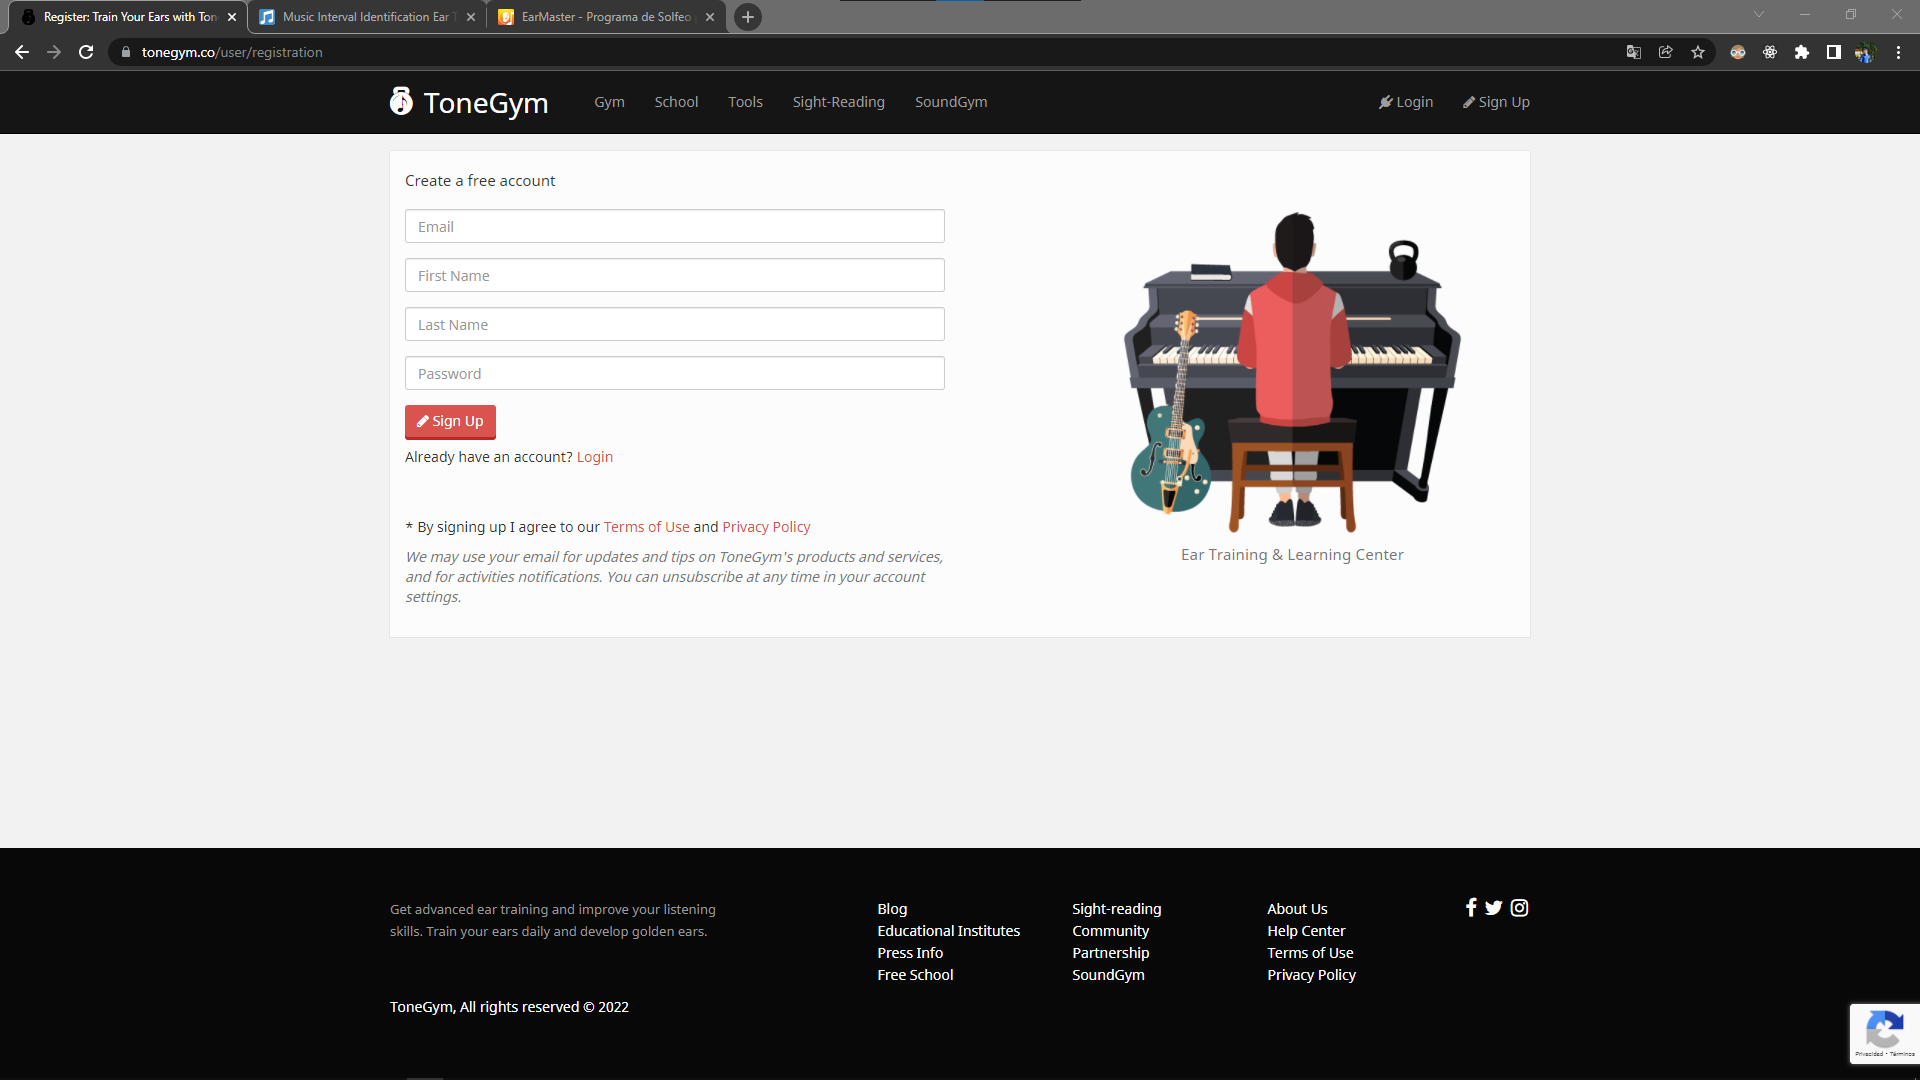
\includegraphics[width=0.45\textwidth]{Estado del Arte/tonegymlogin}}
    \caption{Páginas de inicio de ToneGym.}
    \label{f:ToneGym2}
   \end{figure}
\end{comment}

La sección de ejercicios esta un poco escondida y hay que deslizar hacia abajo para encontrarla. Aunque el diseño está bastante bien, la personalización de los ejercicios es nula. Además, una vez hayas fallado en la respuesta no se te permite continuar probando. Por último, no incorpora ninguna opción para cambiar el instrumento que suena.
\cite{tonegym3}

\subsection{TonedEar}
\label{sec:TonedEar}

Esta aplicación es la que más se parece a lo que queremos construir (ver figura \ref{fig:tonedear}). Contiene varios tipos de ejercicios como identificación de intervalos, escalas, etc. Permite la personalización de los ejercicios mediante un panel a la derecha, aunque no es inmediato. Y ofrece la posibilidad de continuar con el ejercicio aunque falles en la primera respuesta. Además, es una aplicación web gratuita, sencilla, fácil de entender y usar.
\cite{tonedear1}

\begin{figure}[H] 
    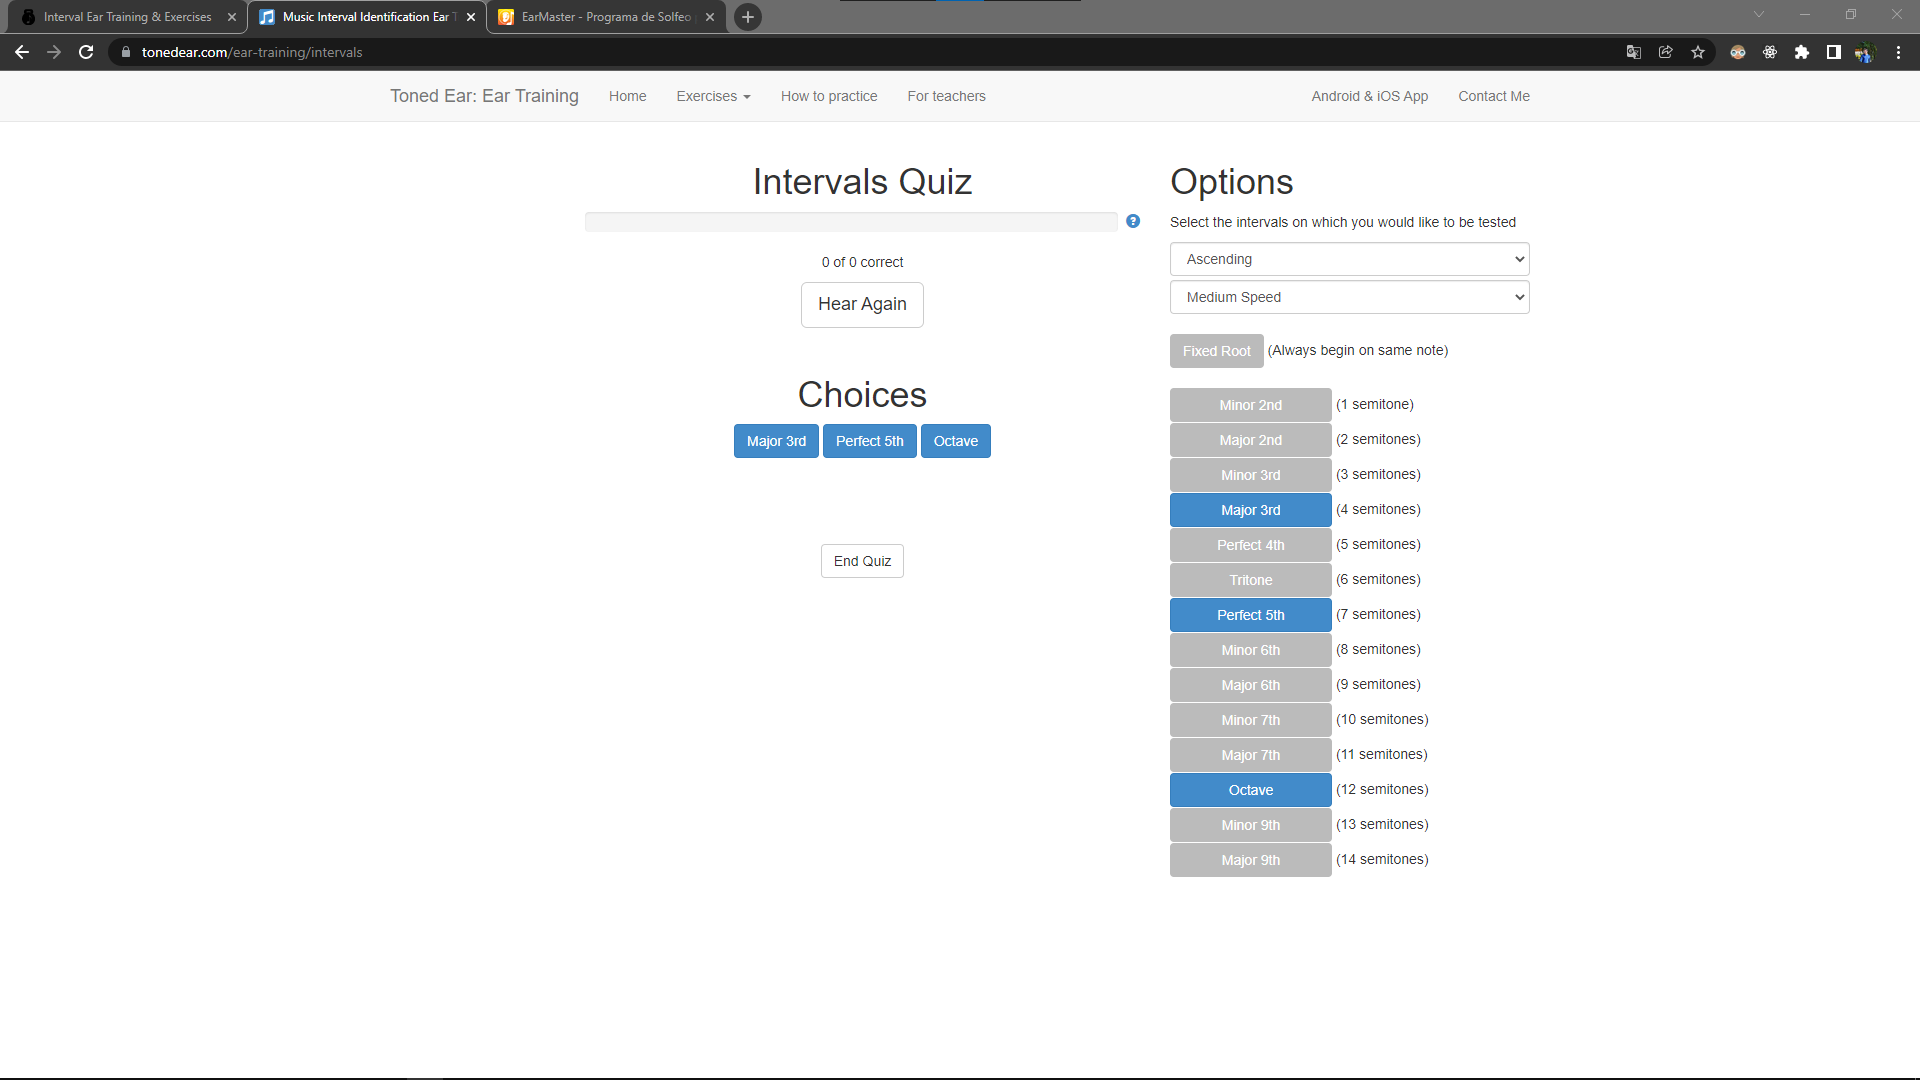
\includegraphics[width=0.9\textwidth]{Estado del Arte/tonedear}
    \centering
    \caption{Página de ejercicio de TonedEar.}
    \label{fig:tonedear}
\end{figure}

Algo que se hace notar analizando el código de la aplicación es que en el ejercicio de identificación de intervalos no se encuentran todos los intervalos posibles. En concreto, una de las dos notas del intervalo será un número MIDI desde 40 hasta 65 y la segunda nota será la primera más un número del 1 al 14. Esto nos da un rango de notas desde 40 hasta 79 cuando el rango de notas MIDI va desde 20 hasta 108 para un piano. Además, puede ocurrir que la primera nota del intervalo suene después de la segunda.

\begin{comment}
\begin{figure}[H] 
    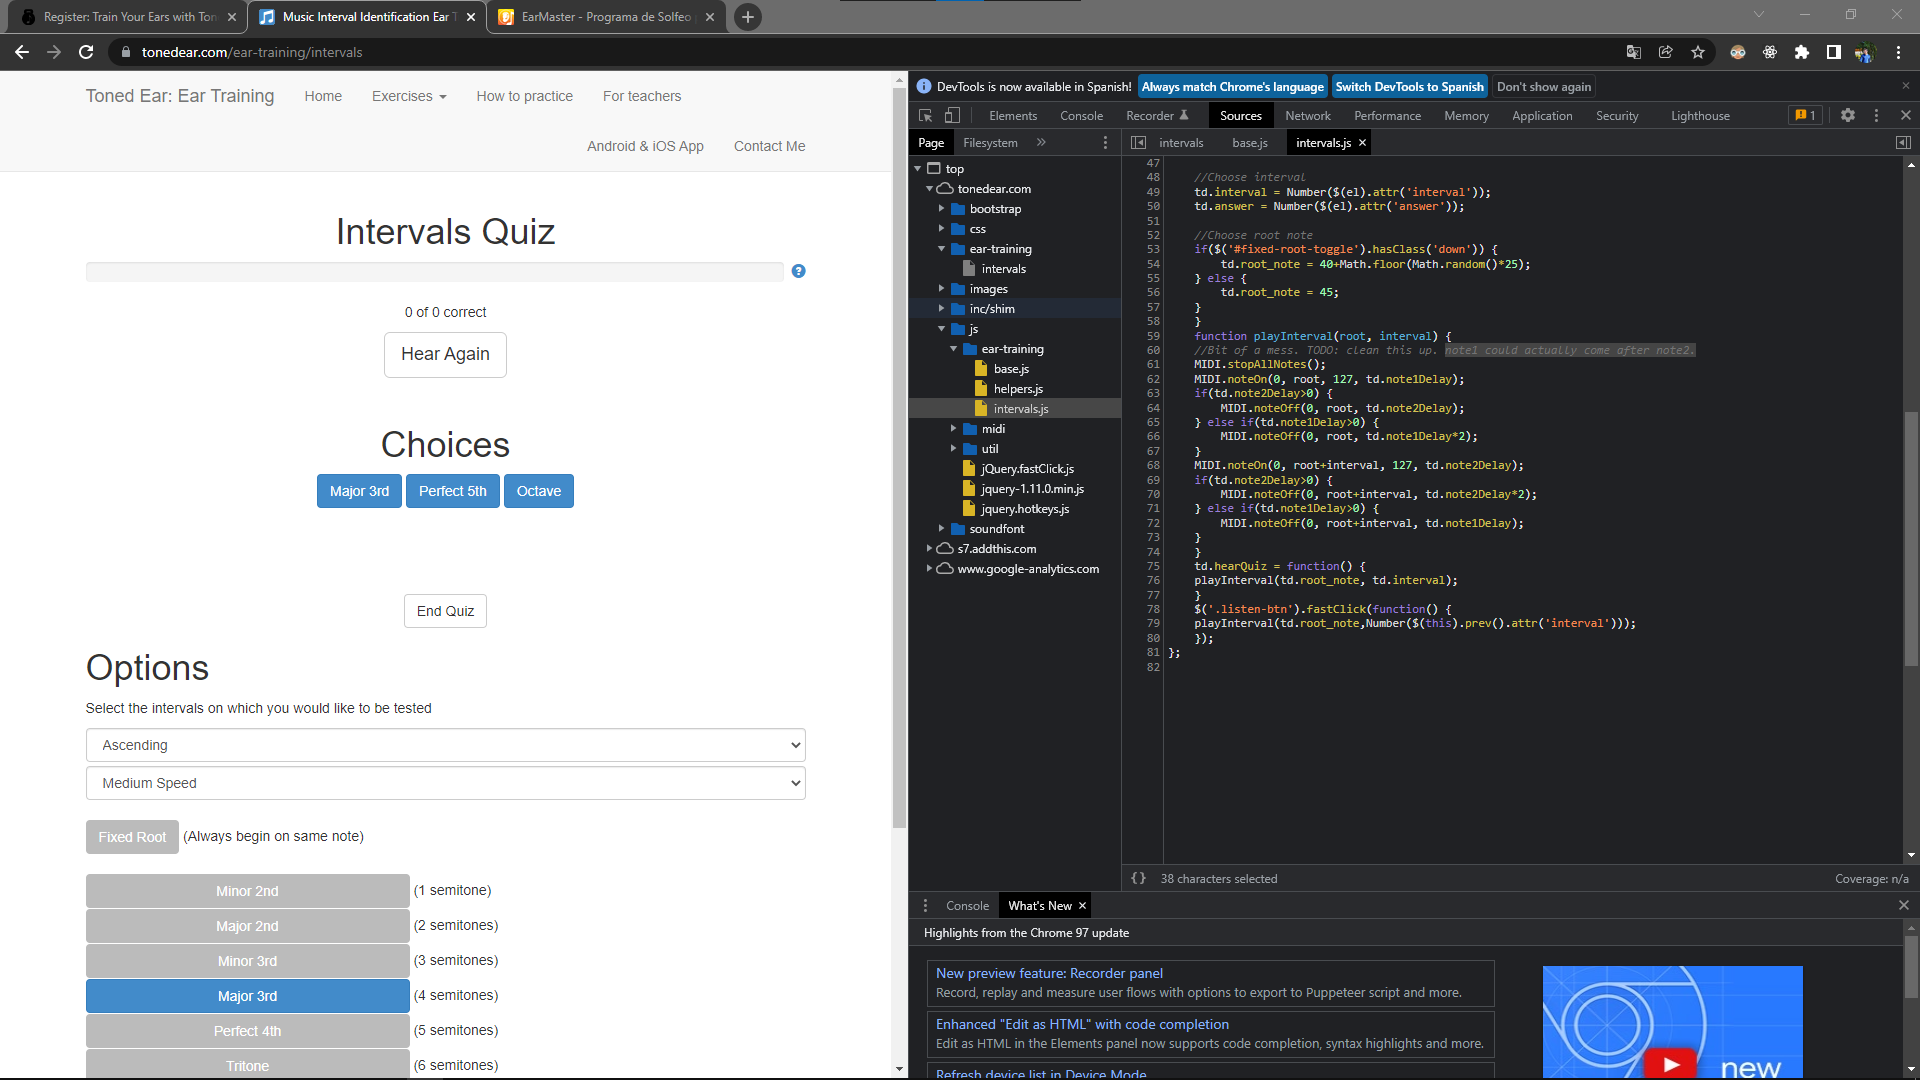
\includegraphics[width=\textwidth]{Estado del Arte/tonedearerror}
    \centering
    \caption{TonedEar Error}
    \label{fig:tonedearerror}
\end{figure}
\end{comment}

Por último, la aplicación permite personalizar los ejercicios pero no permite cambiar entre instrumentos. El instrumento que suena siempre al pulsar el botón de pregunta es un piano.
\cite{tonedear2}

\subsection{EarMaster}
\label{sec:EarMaster}

Parece ser la más completa y elaborada de todas con más de 2500 ejercicios. Contiene ejercicios para que puedas reconocer, transcribir, leer, cantar y tocar: Intervalos, acordes, progresiones armónicas, escalas, ritmos y melodías.
(ver figura \ref{fig:earmaster})
\cite{earmaster1}

\begin{figure}[H] 
    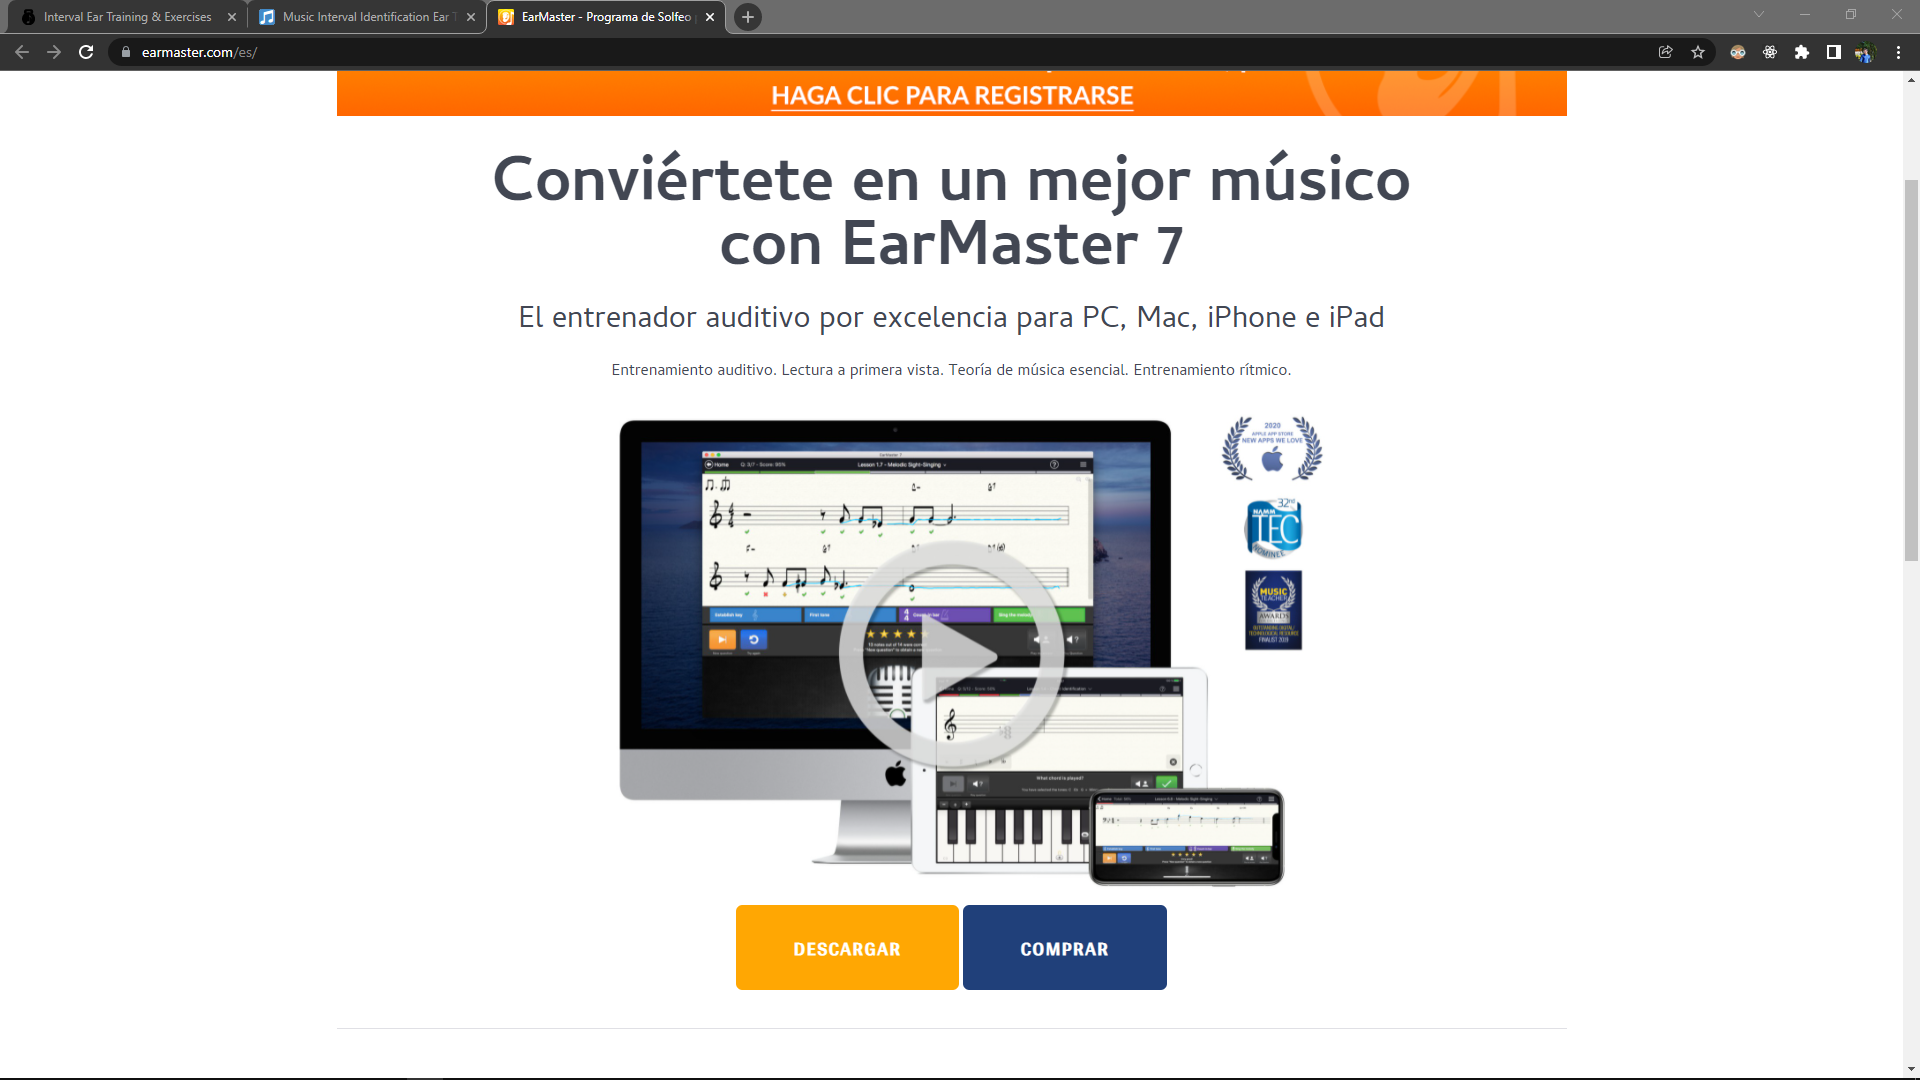
\includegraphics[width=0.75\textwidth]{Estado del Arte/earmaster}
    \centering
    \caption{Página de inicio de EarMaster.}
    \label{fig:earmaster}
\end{figure}

Sin embargo, su contenido gratuito sólo consta de identificación de intervalos y acordes. Para poder hacer uso de la aplicación completa ofrece precios desde los 59,95€ hasta los 99,95€ (ver figura \ref{fig:earmasterprices}). Aparte, necesitas tener la aplicación instalada para utilizarla, no es una aplicación web. Todo esto resulta en que el usuario al que nos estamos enfocando no pueda usarla. Esta aplicación parece estar más destinada a centros educativos que puedan hacerse cargo de la licencia.
\cite{earmaster2}

\begin{figure}[H] 
    
\includegraphics[width=0.85\textwidth]{Estado del Arte/earmasterprices}
    \centering
    \caption{Precios de EarMaster.}
    \label{fig:earmasterprices}
\end{figure}

\section{Objetivos}

El objetivo principal del TFG es desarrollar una aplicación que permita a músicos desarrollar su oído musical mediante el entrenamiento auditivo.

Subobjetivos:
\begin{compactitem}
    \item Desarrollar una interfaz interactiva.
    \item Implementar diferentes tipos de ejercicio personalizables de entrenamiento auditivo. 
    \item Incluir varios instrumentos para prácticar con diferentes sonidos.
\end{compactitem}

\section{Estructura del documento}

Este trabajo se centra en el siguiente proceso combinando de Design Thinking, Lean Startup y Metodologías Ágiles para la creación de un producto mínimo viable (ver figura \ref{fig:LeanDesignAgile}). De esta manera conseguimos un proceso que parte de la nada, se centra en el usuario, gestiona el desarrollo, integra el error y es iterable.
\cite{estructura}

\begin{figure}[H] 
    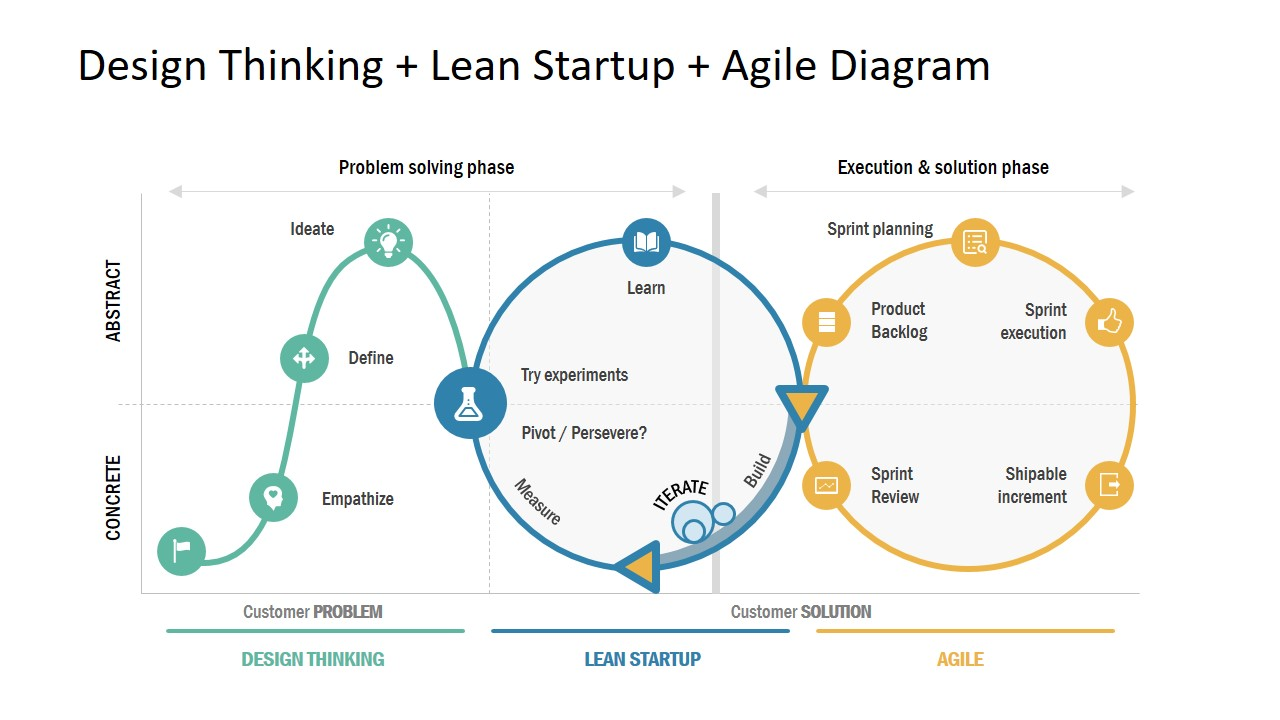
\includegraphics[scale=0.46]{LeanDesignAgile}
    \centering
    \caption{Proceso combinado de Design Thinking, Lean Startup y Agile.}
    \label{fig:LeanDesignAgile}
\end{figure}

Este proceso se ha dividido en la memoria en los siguientes tres capítulos:

\begin{itemize}
    \item \hyperref[sec:diseño]{\textbf{Análisis y Diseño:}} Este capítulo recoge todo lo relacionado con la fase de ideación y puesta en marcha de la solución. Recoge explicaciones del proceso de Design Thinking y Lean Startup. Aquí se pueden encontrar el diseño y el prototipo de la aplicación. %(Ver capítulo \ref{sec:diseño}).
    \item \hyperref[sec:agile]{\textbf{Metodologías Ágiles:}} Este capítulo recoge lo relacionado para llevar a cabo la gestión y desarrollo del software utilizando Scrum y prácticas DevOps. Aquí se puede encontrar cómo se ha realizado la gestión, especificación de requisitos, integración continua y despliegue continuo. %(Ver capítulo \ref{sec:agile}).
    \item \hyperref[sec:desarrollo]{\textbf{Descripción Informática:}} Este capítulo se centra en lo relacionado con la implementación de la solución. Aquí se puede encontrar las tecnologías usadas, los detalles de implementación del código, buenas prácticas y testing. %(Ver capítulo \ref{sec:desarrollo}).
\end{itemize}

Por último, se encuentran las \hyperref[sec:conclusiones]{\textbf{Conclusiones}} derivadas del trabajo con los objetivos alcanzados y una propuesta para trabajos futuros. Y los \hyperref[sec:apendices]{\textbf{Apéndices}}, que complementan la memoria principal con un mayor desarrollo de alguno de sus apartados, capturas de la aplicación e imágenes grandes. %(Ver capítulo \ref{sec:conclusiones} y apéndice \ref{sec:apendices}).
% \afterpage{\blankpage} % puede generar problema en índice de contenidos
% \newpage


%%%%%%%%%%%%%%%%%%%%%%%%%%%%%% 2 Contenidos Principales %%%%%%%%%%%%%%%%%%%%%%%%%%%

\chapter{Análisis y Diseño}
\label{sec:diseño}
Para encontrar una solución viable al problema que se plantea y que aporte un valor real a los usuarios, necesitamos de algún método que nos permita diseñar una solución de manera efectiva bajo unas condiciones de incertidumbre.

Para crear esta propuesta de valor, se puede utilizar \hyperref[sec:design]{\textbf{Design Thinking}} como método de generación de ideas innovadoras y \hyperref[sec:lean]{\textbf{Lean Startup}} como método de aprendizaje validado para la puesta en marcha de la solución.
\cite{analisis}

\section{Design Thinking}
\label{sec:design}

Design Thinking es un método para \textbf{generar ideas innovadoras} que centra su eficacia en entender y dar solución a las necesidades reales de los usuarios. Proviene de la Universidad de Stanford en California (EEUU) y la forma en la que trabajan los diseñadores de producto, de ahí su nombre.
\cite{desingThinking1}

Esta metodología sirve en el proceso de creación para conocer al cliente en profundidad y encontrar soluciones prácticas ante sus problemas de manera ágil. Su objetivo es partir desde las necesidades de los clientes, para generar productos o servicios que las satisfagan.

El proceso de Design Thinking se compone de cinco etapas y no es lineal (ver figura \ref{fig:DesignThinking}). Por tanto, en cualquier momento se puede saltar entre etapas si se cree oportuno. De modo que a lo largo del proceso se va afinando el contenido hasta desembocar en una solución que cumpla con los objetivos. 
\cite{desingThinking2}

Las etapas de Design Thinking son las siguientes:
\begin{compactitem}
    \item \hyperref[sec:empatizar]{\textbf{Empatizar}}: Comprender el entorno y necesidades del usuario. 
    \item \hyperref[sec:definir]{\textbf{Definir}}: Identificar los problemas a solucionar. 
    \item \hyperref[sec:idear]{\textbf{Idear}}: Dar solución a estos problemas. 
    \item \hyperref[sec:prototipar]{\textbf{Prototipar}}: Convertir las soluciones en un prototipo. 
    \item \hyperref[sec:testear]{\textbf{Testear}}: Probar el prototipo con el usuario.
\end{compactitem}

\begin{figure}[H] 
    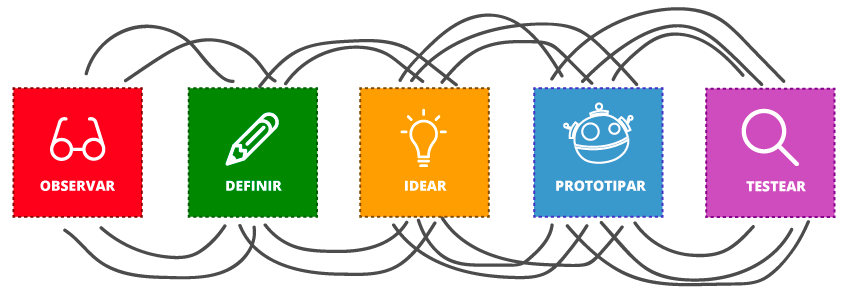
\includegraphics[scale=0.44]{Design Thinking/Etapas}
    \centering
    \caption{Etapas de Design Thinking.}
    \label{fig:DesignThinking}
\end{figure}

\subsection{Empatizar}
\label{sec:empatizar}

Se realizaron entrevistas al usuario y un estudio profundo de teoría musical para entender al usuario y sus necesidades. Además, se analizaron diversas herramientas ya existentes de entrenamiento musical como se ha explicado en el estado del arte. Se puede encontrar una explicación más detallada en el apéndice \hyperref[sec:DesignThinking]{\textbf{A.2 Design Thinking}}.

\subsection{Definir}
\label{sec:definir}

El problema parte de la necesidad de músicos amateur que quieren mejorar su nivel de percepción de la música. Sin los medios adecuados resulta imposible llevar a cabo el entrenamiento auditivo que es una parte fundamental para llevar a cabo su propósito. 

\subsection{Idear}
\label{sec:idear}

Para idear una solución que aporte valor, realizamos un \textbf{MindMap} \cite{mindmap} donde nos enfocamos en los principales problemas del usuario y sus posibles soluciones.
Cómo se puede observar en la figura \ref{fig:Mindmap}, se concluye que una posible forma de solucionar estos problemas es mediante una aplicación web con ejercicios de entrenamiento auditivo. 

\begin{figure}[H]
    \centering
    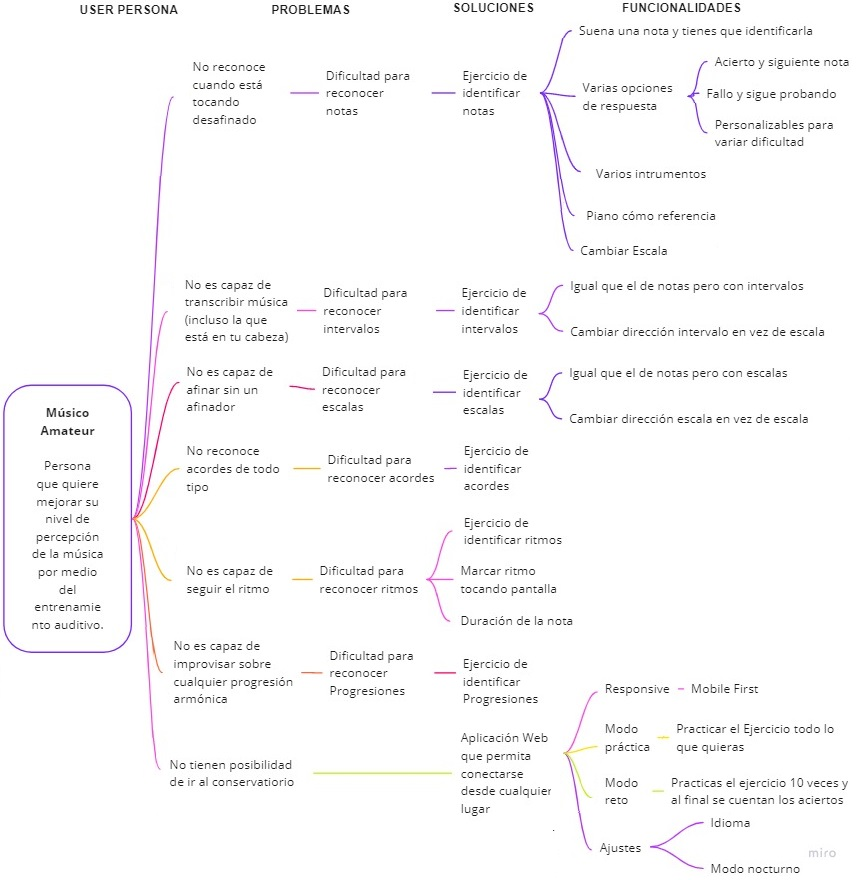
\includegraphics[scale=0.47]{Design Thinking/MindMap}
    \caption{MindMap de los principales problemas y soluciones.} 
    \label{fig:Mindmap}
\end{figure}

\subsection{Prototipar}
\label{sec:prototipar}

Primero, utilizamos la técnica \textbf{MoSCoW} \cite{moscow} para establecer las prioridades del proyecto. Teniendo en cuenta nuestras limitaciones: poco tiempo para desarrollar, aprender conceptos musicales y nuevas tecnologías. 
(Ver figura \ref{fig:MoSCoW}).

\begin{figure}[H]
    \centering
    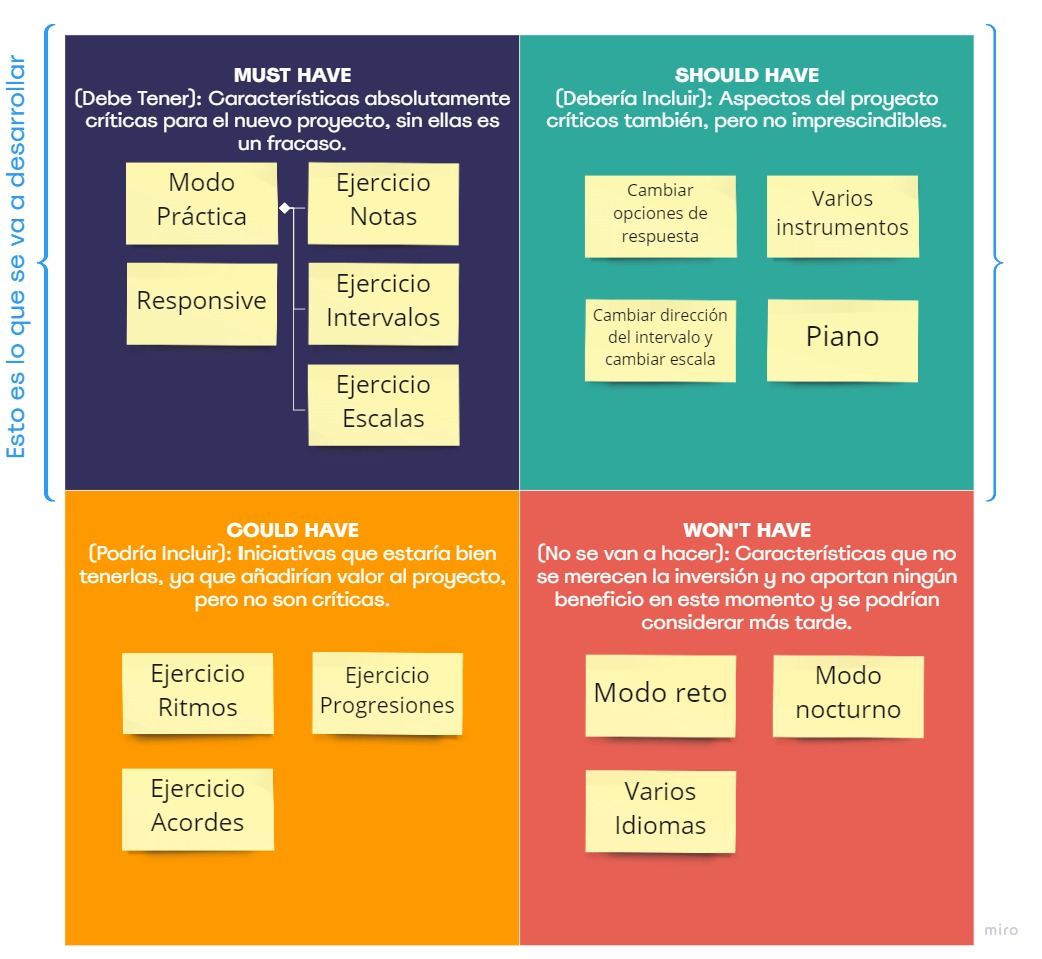
\includegraphics[scale=0.35]{Design Thinking/MosCow}
    \caption{Método MoSCoW con las prioridades del proyecto.}
    \label{fig:MoSCoW}
\end{figure}

Después, para crear nuestro \textbf{producto mínimo viable} o decidimos centrarnos en desarrollar lo que debe tener (Must have) y más tarde lo que debería tener (Should have).

Por último, una vez establecidas las prioridades del proyecto pasamos a visualizarlas diseñando el prototipo teniendo en cuenta la filosofía de diseño \textbf{Mobile First} \cite{mobilefirst}. Diseñando primero para pantallas pequeñas y después adaptándolo a pantallas más grandes. 

\begin{figure}[H]
    \centering
    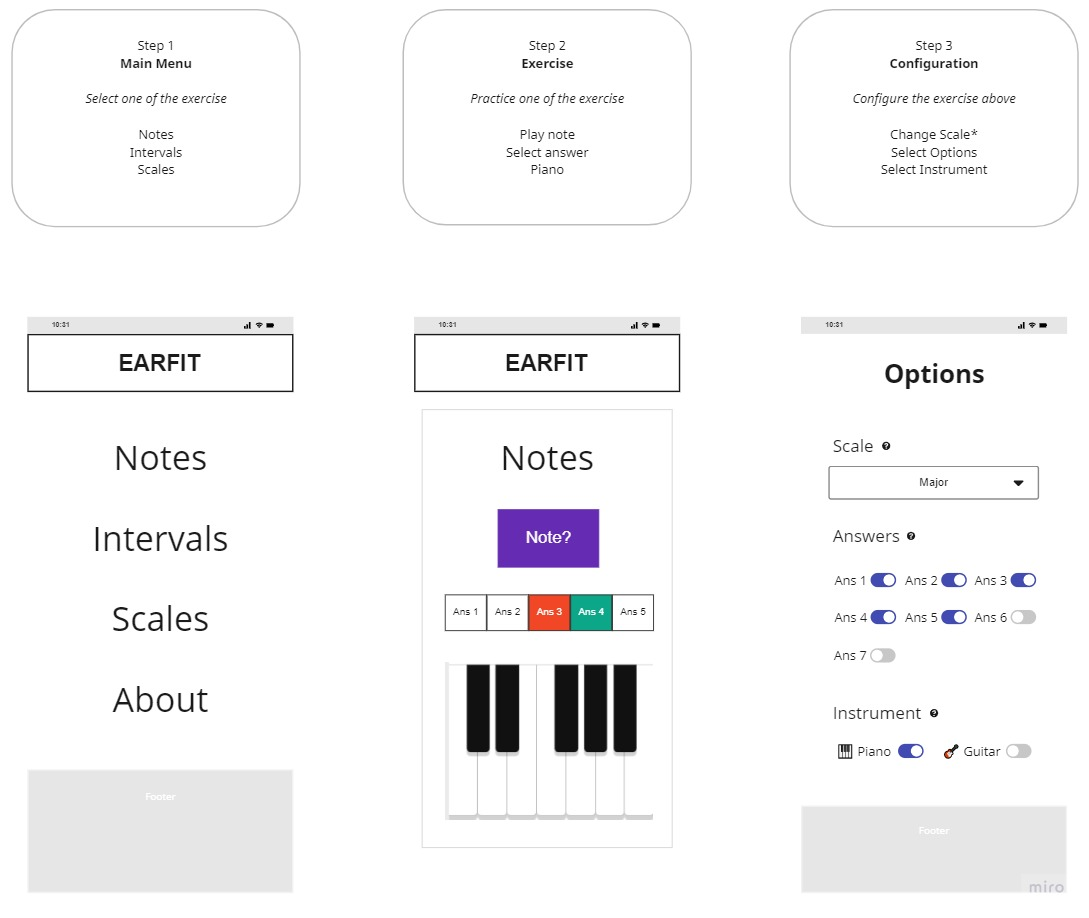
\includegraphics[width=\textwidth]{Design Thinking/Prototipo/Small/Prototipo}
    \caption{Prototipo para pantallas pequeñas.}
    \label{fig:PrototipoSmall}
\end{figure}

En la figura \ref{fig:PrototipoSmall} se puede apreciar una pequeña parte del prototipo para pantallas pequeñas. Todos los demás diseños del prototipo incluyendo pantallas pequeñas, medias y grandes se pueden encontrar en el apéndice \hyperref[sec:Prototipos]{\textbf{B. Prototipos}}.

\subsection{Testear}
\label{sec:testear}

Después de haber testeado los primeros diseños con el usuario, haber hecho correcciones y haber validado el último prototipo que hemos visto anteriormente, pasamos a crear la solución aplicando el método \textbf{Lean Startup}.

\section{Lean Startup}
\label{sec:lean}

Es un método riguroso para \textbf{agilizar la puesta en marcha} de soluciones y optimizarlas con base en un proceso de aprendizaje y de corrección iterativa. Comenzó con el método de desarrollo de clientes y el método Lean en los sistemas de fabricación japoneses popularizado por Toyota.

La metodología Lean Startup se basa en el circuito de feedback de información: \textbf{crear, medir, aprender} (ver figura \ref{fig:LeanStartup}). Crear una hipótesis, diseñar un experimento (producto mínimo viable) para testear esa hipótesis, llevar a cabo el experimento, reunir datos, reflexionar y ver si validan o rechazan la hipótesis para pivotar.
\cite{leanstartup1}

\begin{figure}[H]
    \centering
    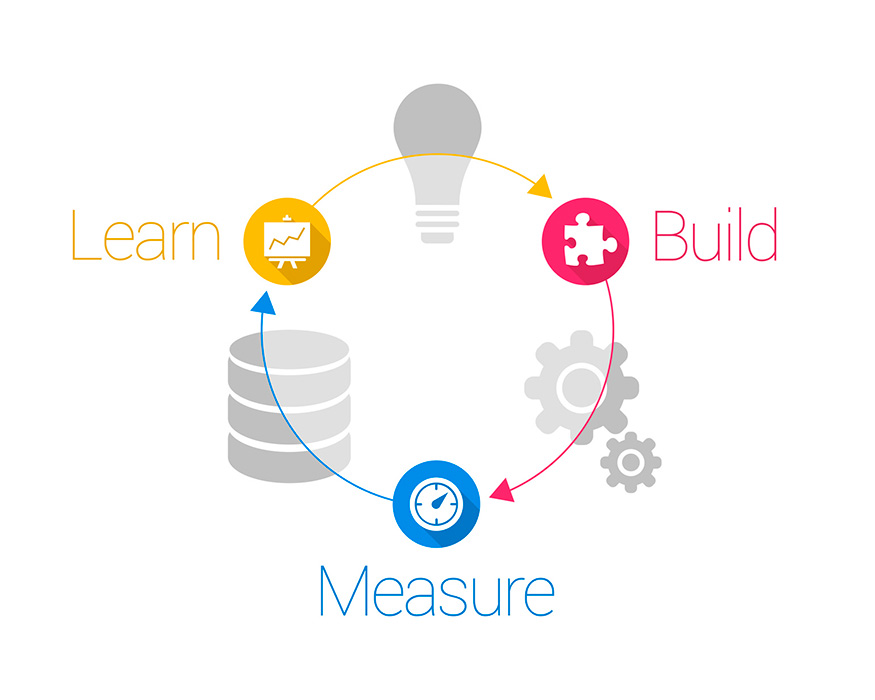
\includegraphics[scale=0.3]{Lean Startup/CircuitoFeedback}
    \caption{Circuito de feedback de información.}
    \label{fig:LeanStartup}
\end{figure}

Lean Startup sirve para acortar los ciclos de desarrollo, medir el progreso y ganar feedback por parte de los usuarios. Esto se consigue porque se basa en el aprendizaje validado, la experimentación científica y la iteración en los lanzamientos del producto. 
Debido a esto es considerado una herramienta imprescindible para la puesta en marcha de soluciones software. 

Para no extender este trabajo se puede encontrar una explicación detalla de como fue este proceso de crear, medir, aprender en el apéndice \hyperref[sec:LeanStartup]{\textbf{A.3 Lean Startup}}. A continuación, nos centraremos sólo en la fase de creación del software.
\cite{leanstartup2}

Después haber establecido nuestra hipótesis y diseñado un producto mínimo viable usando \textbf{Design Thinking} pasamos a desarrollarlo aplicando \textbf{Metodologías Ágiles}.

\chapter{Metodologías Ágiles}
\label{sec:agile}
Para gestionar el desarrollo del software de manera exitosa necesitamos asegurar un proceso visible, controlado, repetitivo, eficiente y predecible. Necesitamos adaptar las formas de trabajo a las necesidades del proyecto, prolongando respuestas rápidas y flexibles para acomodar el desarrollo.

La agilidad es la habilidad, que facilita la adaptación, de manera rápida y efectiva en circunstancias cambiantes, para garantizar la entrega de valor continuo, en ciclos cortos de tiempo y con el mínimo coste. \cite{manifiestoAgil} %(Ver apéndice \ref{sec:ManifiestoAgil}).

Para ser ágiles mientras desarrollamos podemos beneficiarnos de \hyperref[sec:DevOps]{\textbf{DevOps}} como filosofía de desarrollo y \hyperref[sec:Scrum]{\textbf{Scrum}} como modelo organizativo.
\cite{agile}

\section{Scrum}
\label{sec:Scrum}

Scrum es un \textbf{proceso de gestión} que reduce la complejidad en el desarrollo de productos para satisfacer las necesidades de los clientes. Se considera un marco de gestión de proyectos ágil.

Con Scrum, un producto se basa en una serie de iteraciones llamadas \textbf{sprints} que dividen proyectos grandes y complejos en partes más pequeñas. Priorizadas por el beneficio que aportan al receptor del producto.
\cite{scrum1}

El flujo de trabajo en Scrum como se ilustra en la figura \ref{fig:Scrum} es el siguiente:

\begin{enumerate}
    \item Un Product Owner ordena el trabajo de un problema complejo en un Product Backlog.
    \item El Equipo Scrum convierte una selección del trabajo en un Incremento de valor durante un Sprint.
    \item El Equipo Scrum y sus partes interesadas inspeccionan los resultados y se ajustan para el próximo Sprint.
    \item \textit{Repetir}
\end{enumerate}

\textbf{Scrum no es} un proceso o una técnica para desarrollar/construir productos, realmente es un marco de trabajo donde podemos emplear un conjunto de diferentes procesos y técnicas.

\begin{figure}[H]
    \centering
    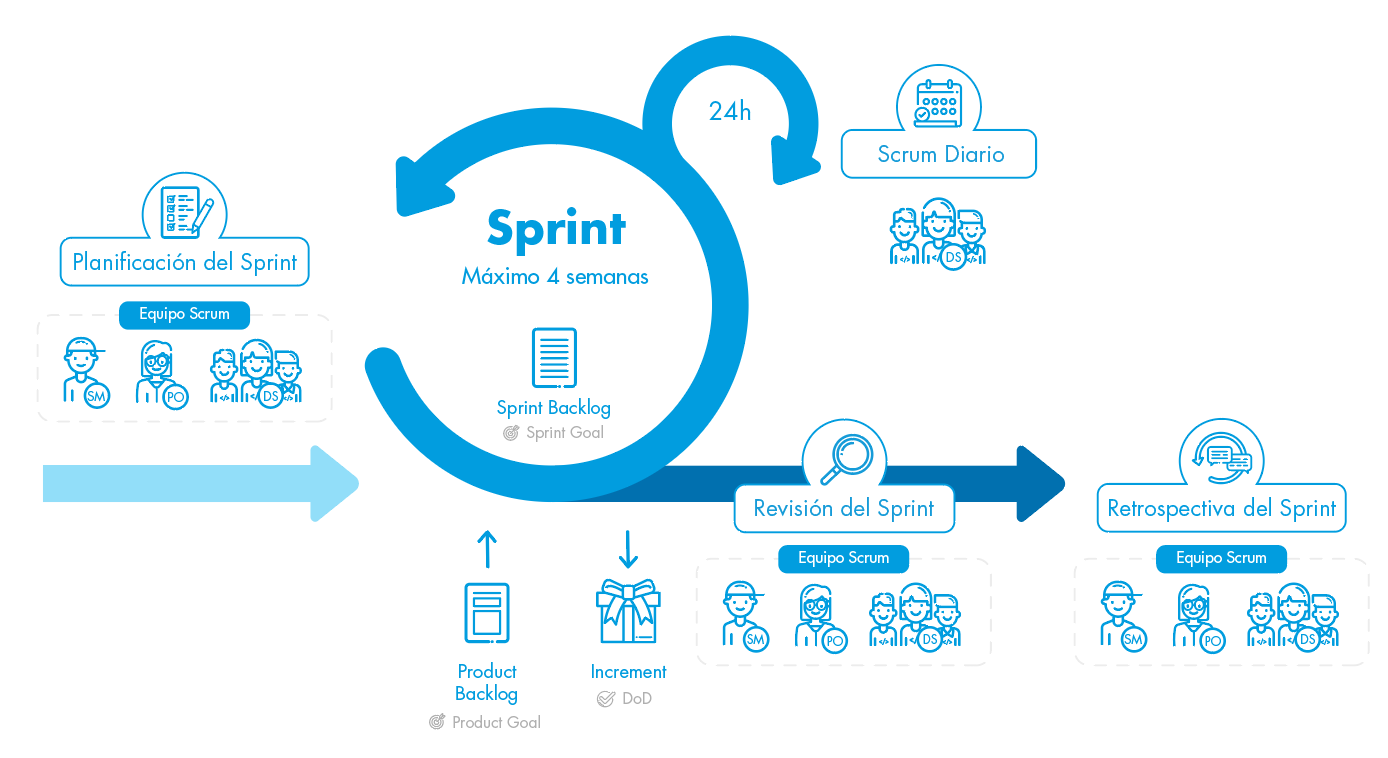
\includegraphics[scale=0.39]{Scrum/Scrum}
    \caption{Marco de trabajo Scrum.}
    \label{fig:Scrum}
\end{figure}

Implementar este marco de trabajo nos permite obtener resultados pronto, reduciendo el \textbf{Time to Market}, es decir, a tener lo antes posible en el mercado nuestro producto o una característica de nuestro producto, aumentando la satisfacción del cliente. Además, permite lidiar con requisitos cambiantes o poco definidos, aportando tolerancia al cambio.

Es ideal para crear nuevos productos poniendo el foco en el cliente y detectar fallos pronto. Lo que se traduce en una mayor calidad del producto, reducción de costes y optimización del riesgo.
\cite{scrum2}

\subsection{User Story Map}

Es un método de mapeo de UX (experiencia de usuario) que se utiliza para delinear las interacciones que se espera que realicen los usuarios para completar sus objetivos en un producto digital. Ayuda a definir el \textbf{viaje o casos de uso} del usuario en el producto.
\cite{userStoryMap1}
\cite{userStoryMap2}
\cite{userStoryMap3}

\begin{figure}[H]
    \centering
    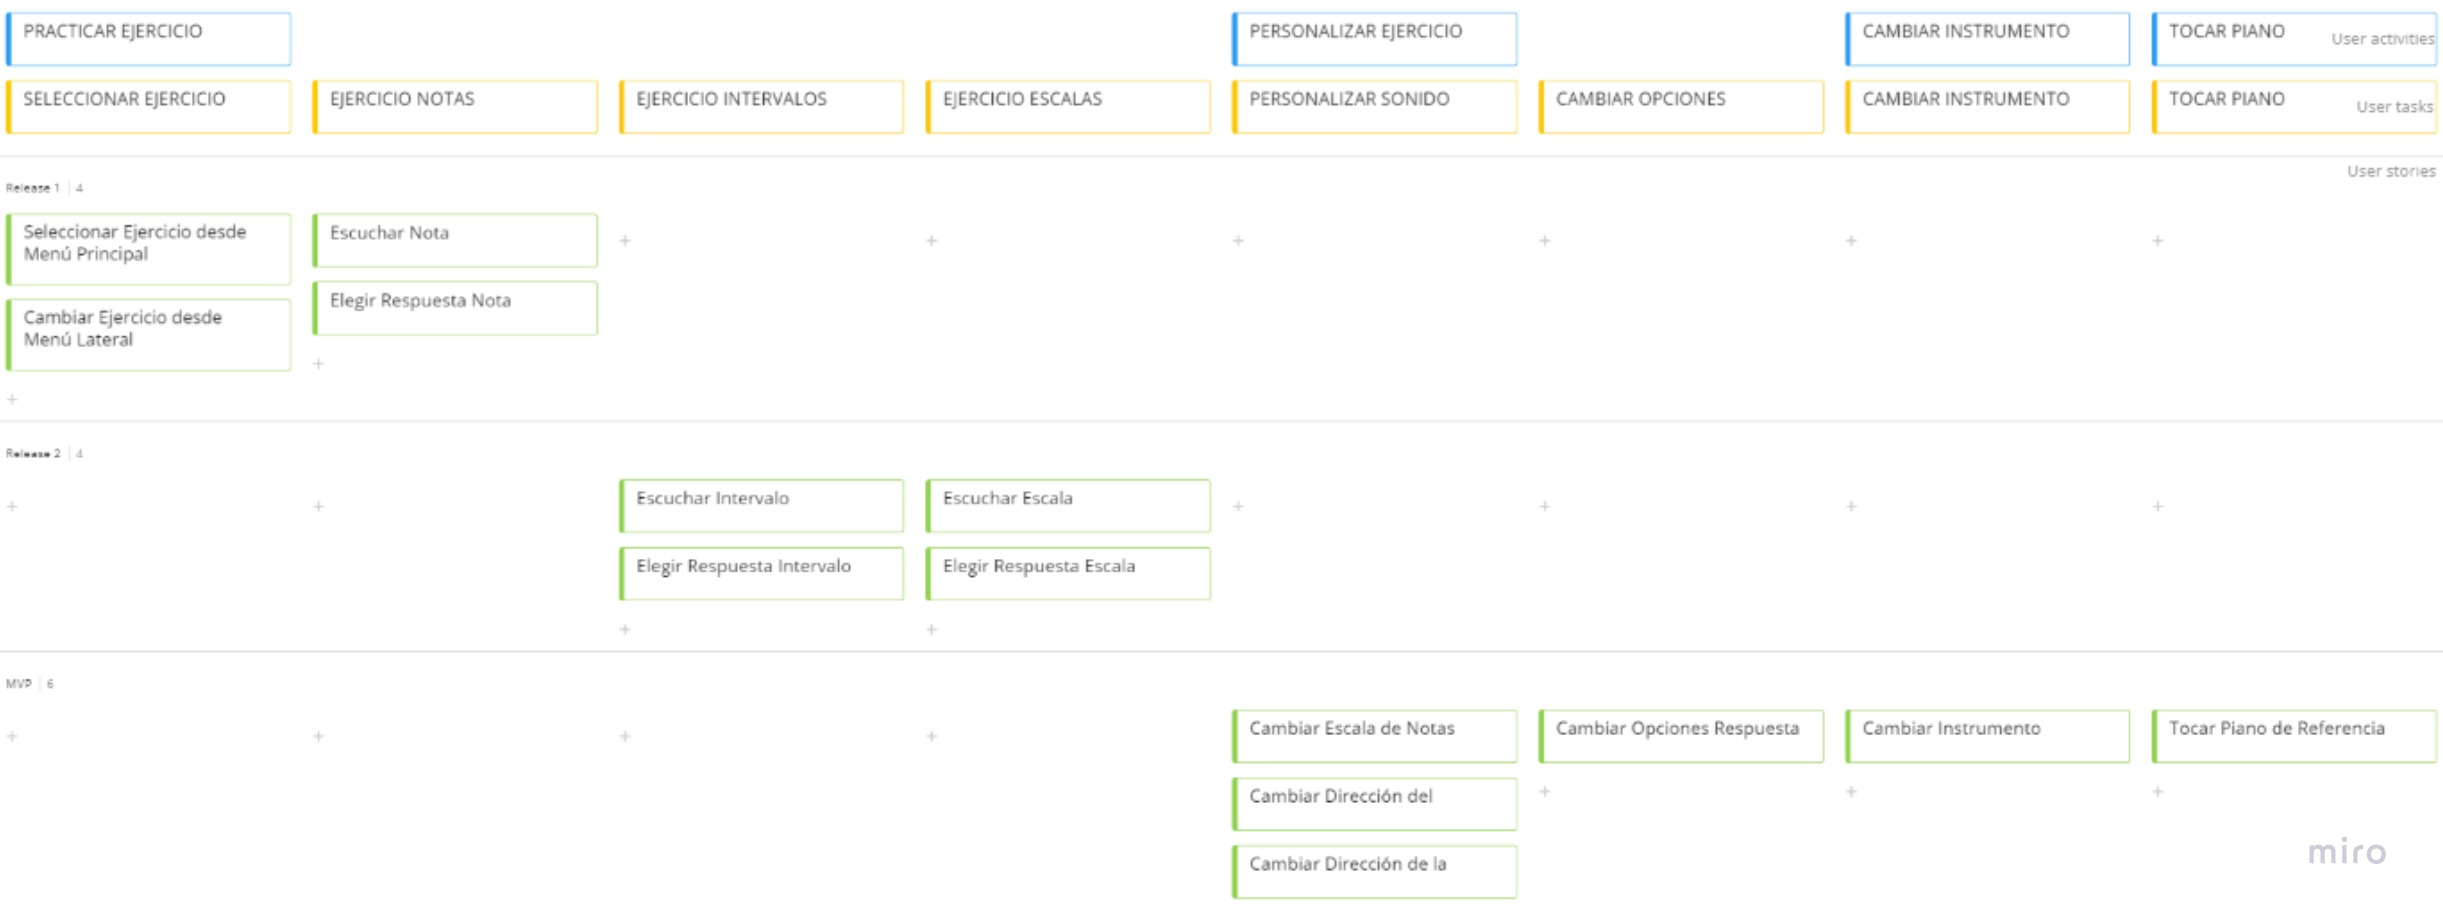
\includegraphics[width=\textwidth]{Scrum/UserStoryMap}
    \caption{User Story Map del producto.}
    \label{fig:UserStoryMap}
\end{figure}

En la figura \ref{fig:UserStoryMap} podemos observar el User Story Map o mapa de historias de usuario del producto. Este User Story Map representa 3 tipos de acciones:
\begin{itemize}
    \item Las \textbf{User Activities}: Representan las tareas de alto nivel que los usuarios pretenden completar en el producto. Son los principales objetivos del usuario en la aplicación. 
    \item Las \textbf{User Task}: Representan las subtareas específicas que los usuarios realizarán en el producto para completar la actividad superior. Son las actividades a realizar por el usuario y siguen un flujo narrativo. 
    \item Las \textbf{User Stories} o historias de usuario: Describen las interacciones concretas que experimentarán los usuarios para completar el paso anterior. Definen las funcionalidades del producto y están agrupadas por releases.  
\end{itemize}

Las User Activities y User Task se muestran horizontalmente en la parte superior y las User Stories se apilan verticalmente debajo en orden de prioridad.

Se recomienda visitar este mural de Miro, donde se puede encontrar este roadmap junto con más esquemas y diseños de la aplicación, en el siguiente enlace: 

\href{https://miro.com/app/board/uXjVOMmPLjM=/?share_link_id=588058562303}{https://miro.com/app/board/uXjVOMmPLjM=/}

\subsection{Scrum Board}

Es un método para \textbf{visualizar el trabajo} y gestionar el desarrollo. Esto nos permite separar en pequeñas tareas cada historia de usuario y minimizar los riesgos de entrega. Realizando una construcción iterativa incremental donde se integra al final de cada sprint para validar el resultado. 
\cite{scrumboard1}
\cite{scrumboard2}

\begin{figure}[H]
    \centering
    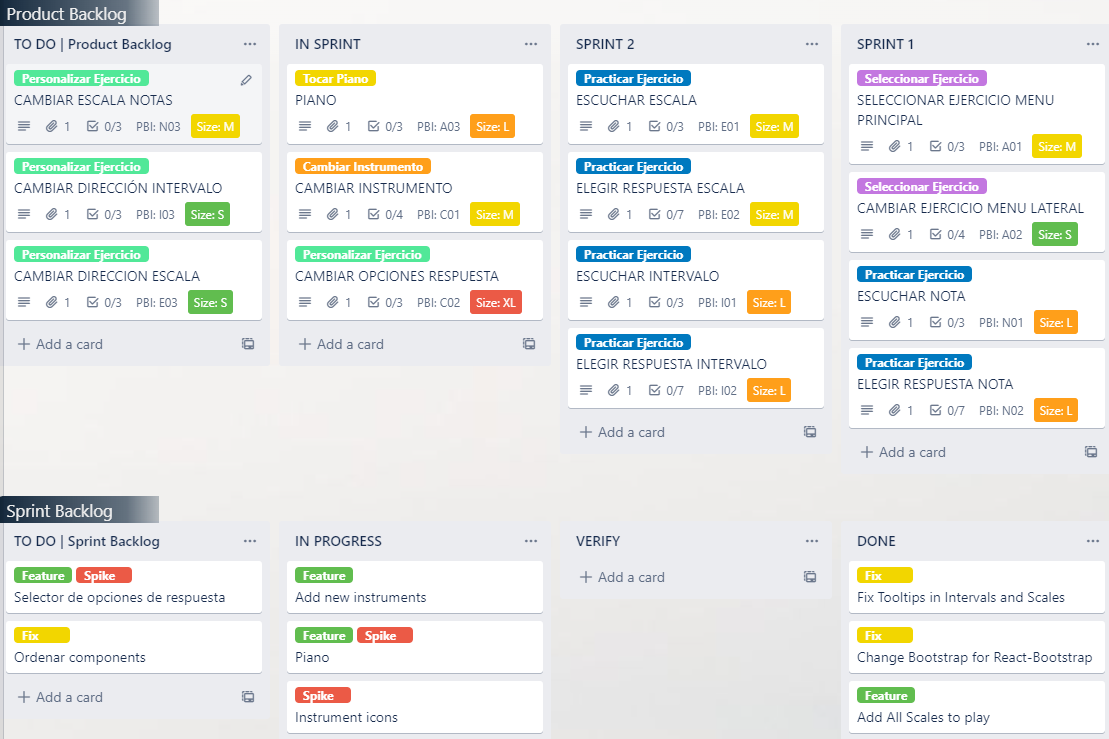
\includegraphics[scale=0.47]{Scrum/ScrumBoard}
    \caption{Scrum Board con el Product Backlog y Sprint Backlog.}
    \label{fig:ScrumBoard}
\end{figure}

En la figura \ref{fig:ScrumBoard} podemos observar el Scrum Board del proyecto en un punto a mitad del desarrollo. Este Scrum Board está compuesto por:
\begin{itemize}
    \item El \textbf{Product Backlog}: Es la lista de todas las tareas o historias de usuario detalladas pendientes para el desarrollo. Es una evolución de los documentos de requisitos tradicionales y desglosa el roadmap del producto en un documento vivo de tareas realizables.
    \item El \textbf{Sprint Backlog}: Es una lista con todas las tareas técnicas que se compromete a llevar a cabo dentro de un Sprint. Cada historia de usuario se divide en estas tareas más pequeñas a completar. Estas tareas pasan por diferentes etapas hasta completarse.
\end{itemize}

Este Scrum Board se puede visitar en el siguiente enlace: 

\url{https://trello.com/b/ZnsnNP2h/earfit}.

\subsection{User Stories}

Las historias de usuarios son descripciones breves y sencillas de las \textbf{características o requisitos} del sistema contadas desde la perspectiva del usuario o cliente del sistema. Cada una es un incremento en el valor del producto.
\cite{userstories1}
\cite{userstories2}

\begin{figure}[H]
    \centering
    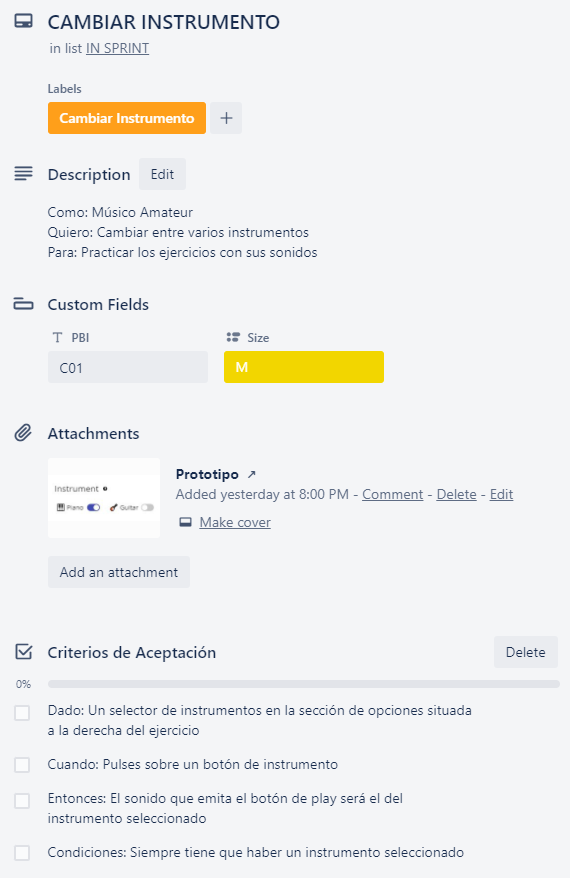
\includegraphics[width=0.64\textwidth]{Scrum/UserStory}
    \caption{Historia de usuario ``Cambiar Instrumento''.}
    \label{fig:UserStory}
\end{figure}

En la figura \ref{fig:UserStory} se puede observar una de las historias de usuario. Todas siguen el método INVEST para garantizar que ofrecen valor. Y el método SMART para descomponerlas en tareas. \cite{invest}
 
\begin{comment}
Estas historias se componen de:
\begin{itemize}
    \item Una \textbf{Etiqueta} que la asocia a una User Activity de alto nivel.
    \item Una \textbf{Descripción} que sigue la estructura “Como [rol], Quiero [objetivo], Para [motivación]”
    \item Una \textbf{Código Identificador} y \textbf{tamaño}, que es una estimación del tiempo que llevará desarrollarla.
    \item Unos \textbf{Criterios de aceptación} que validan la implementación y la dan por completada.
\end{itemize}
\end{comment}

Estas historias de usuario se encuentran en el apéndice \hyperref[sec:UserStories]{\textbf{C. Historias de Usuario}}. También se pueden ver en el ScrumBoard en el siguiente enlace: 

\url{https://trello.com/b/ZnsnNP2h/earfit}.


\section{DevOps}
\label{sec:DevOps}

DevOps, es una combinación de los términos desarrollo (development) y operaciones (operations), significa la unión de personas, procesos y tecnología para ofrecer valor a los clientes de forma constante.

Se enfoca en \textbf{agilizar los procesos} con los que una nueva funcionalidad, mejora o corrección pasa del desarrollo a la implementación, a un entorno de producción que pueda generar valor para el usuario.
(Ver figura \ref{fig:DevOps}).

%Algunas de las formas en las que los equipos de DevOps planean con agilidad y visibilidad son la creación de registros de trabajo pendiente, seguimiento de errores, administración ágil con Scrum, uso de tableros Kanban y visualización del progreso entre otros.
Algunas de las prácticas recomendadas de DevOps que ya se han visto son: la gestión de proyectos de manera ágil con Scrum, creación de registros de trabajo pendiente, visualización del progreso y recopilación de feedback continuo entre otros.

El desarrollo de \textbf{aplicaciones modernas} requiere procesos diferentes a los enfoques del pasado. Las nuevas empresas utilizan enfoques ágiles para desarrollar sistemas de software.
\cite{devops1}

\begin{figure}[H]
    \centering
    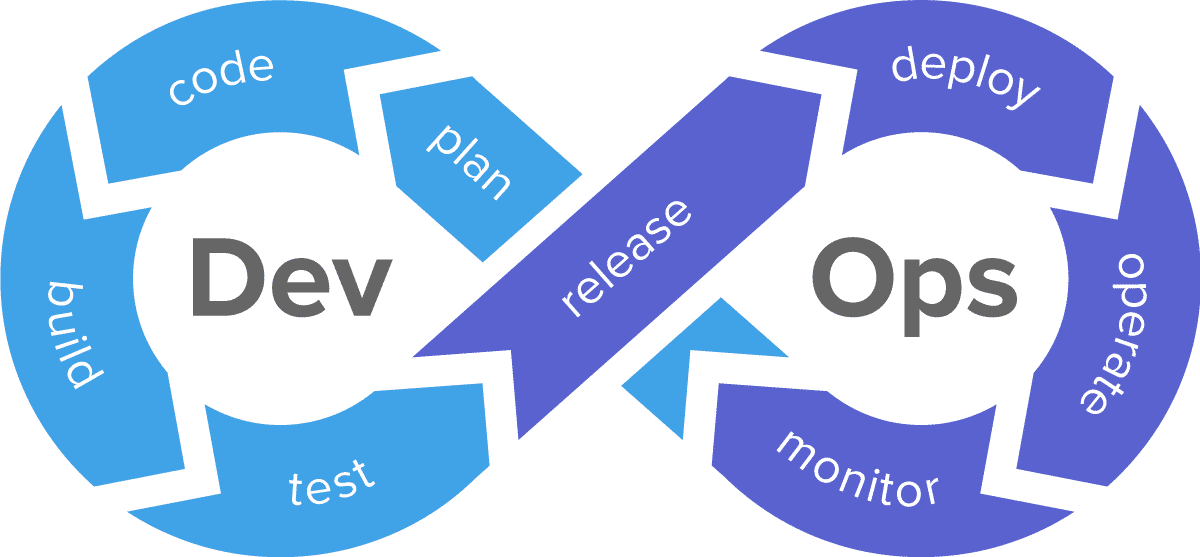
\includegraphics[width=0.68\textwidth]{DevOps/DevOps}
    \caption{Diagrama de DevOps.}
    \label{fig:DevOps}
\end{figure}

DevOps permite fabricar software más rápidamente, con mayor calidad, menor coste y una alta frecuencia de releases. Al adoptar prácticas de DevOps, se asegura la confiabilidad, la alta disponibilidad y el objetivo de ningún tiempo de inactividad del sistema.

El primero de los 12 principios del Manifiesto Ágil es el siguiente: ``Satisfacer a los clientes mediante la distribución de software continua y oportuna'' \cite{manifiestoAgil}. Este es uno de los motivos por el que es importante aplicar prácticas de DevOps, cómo la \hyperref[sec:ic]{\textbf{Integración Continua}} y el \hyperref[sec:dc]{\textbf{Despliegue Continuo}}.
\cite{devops2}

\subsection{Integración Continua (CI)}
\label{sec:ic}

La integración continua es una práctica de DevOps mediante la cual los desarrolladores combinan los cambios en el código en un repositorio central de forma periódica. Para implantar integración continua se suele definir un ``pipeline'', es decir, un conjunto de etapas y de fases automátizadas por las que va pasando el software hasta integrarse con el resto. 
\cite{ic}

En nuestro caso usamos \textbf{Github} \cite{github}, que es un servicio basado en la nube, cómo herramienta de control de versiones \textbf{Git} \cite{git}. Y utilizamos \textbf{Gitflow} \cite{gitflow}, que es un modelo alternativo de creación de ramas en Git como se ilustra en la Figura \ref{fig:Gitflow}.

\begin{figure}[H]
    \centering
    \includegraphics[scale=0.58]{DevOps/Gitflow}
    \caption{Modelo de creación de ramas Gitflow.}
    \label{fig:Gitflow}
\end{figure}

El funcionamiento de este modelo se caracteriza por el uso de varias ramas de función, una rama de desarrollo y una rama de producción:

\begin{itemize}
    \item \textbf{Ramas de Función:} Cada una de estas ramas se crea desde la rama de desarrollo para implementar una nueva funcionalidad del sistema.
    \item \textbf{Rama de Desarrollo:} Cada vez que una rama de funcionalidad es completada se une a ésta integrando los nuevos cambios.
    \item \textbf{Rama de Producción:} Cada vez que una nueva versión está lista en la rama de desarrollo se une a ésta generando una nueva release.
\end{itemize}

\subsection{Despliegue Continuo (CD)}
\label{sec:dc}

El despliegue continuo es una estrategia de DevOps en la que los cambios de código de una aplicación se publican automáticamente. Es útil para entregar funcionalidades del software de forma frecuente.
\cite{dc}

Para ello utilizamos \textbf{GitHub Actions} \cite{githubActions} el cuál nos permite personalizar y automatizar estos despliegues desde nuestro repositorio. Y para alojar nuestra aplicación web usamos \textbf{Vercel}, que es una plataforma en la nube optimizada para proyectos \textbf{Nextjs} \cite{vercelNext}.

\begin{figure}[H]
    \centering
    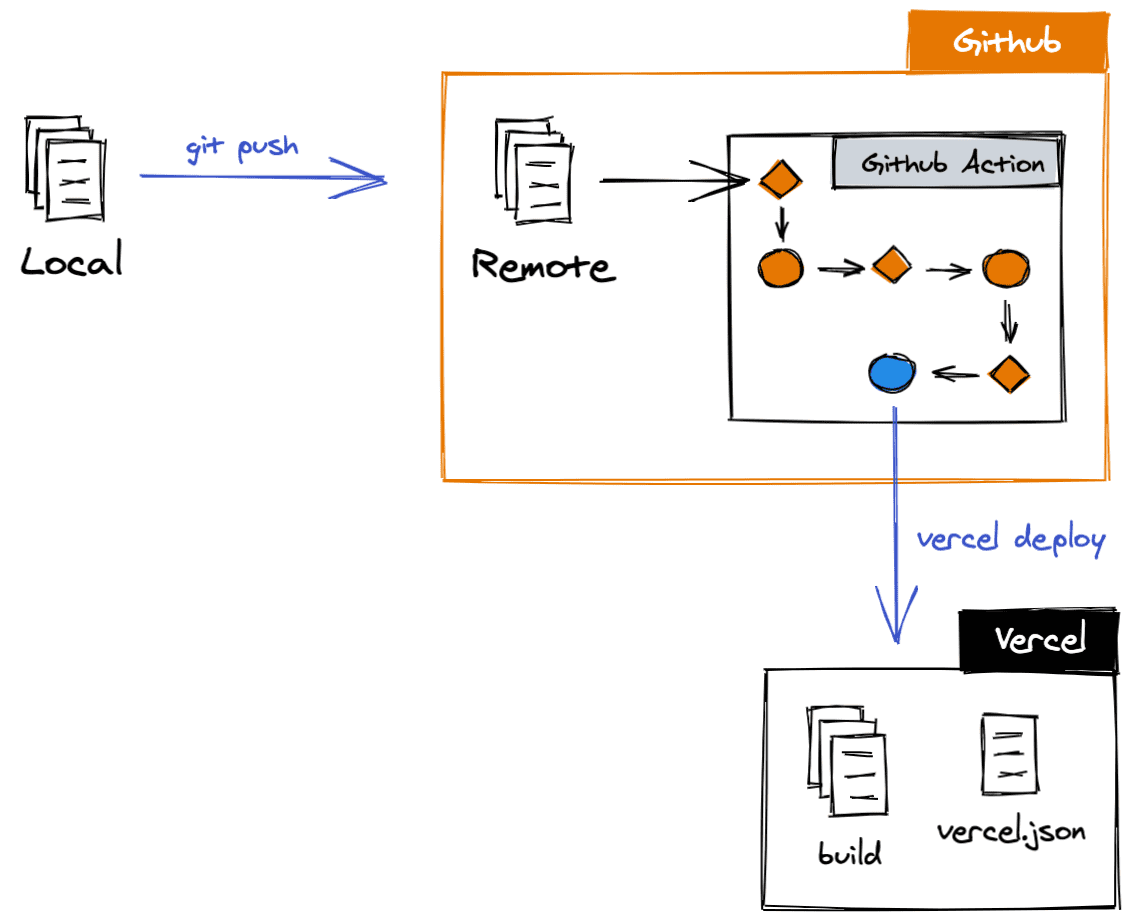
\includegraphics[scale=0.3]{DevOps/DPS}
    \caption{Flujo de trabajo DPS: Develop, Preview and Ship.}
    \label{fig:vercel_workflow}
\end{figure}

Cada vez que se realiza una subida de código, Github Actions hace un despliegue en Vercel siguiendo el \textbf{flujo de trabajo DPS} \cite{dps} (ver Figura \ref{fig:vercel_workflow}):

\begin{itemize}
    \item \textbf{Desarrollo}: Escribimos código en Next.js y subimos los cambios a una rama en Github.
    \item \textbf{Vista previa}: Vercel crea un despliegue de cada rama que estará disponible a través de una URL. Podemos compartir esta URL con otros para recibir feedback. 
    \item \textbf{Enviar a Producción}: Fusionamos la rama creada con la rama ``main'' para enviar a producción.
\end{itemize}


\chapter{Descripción Informática}
\label{sec:desarrollo}

Para desarrollar una aplicación de calidad es necesario el uso de unas guías de estándares de calidad de código, un moderno stack tecnológico, así como buenas prácticas. A continuación se encuentra una detallada descripción informática incluyendo \hyperref[sec:stack]{\textbf{tecnologías}}, \hyperref[sec:implementacion]{\textbf{implementación}} y \hyperref[sec:pruebas]{\textbf{pruebas}}.

\section{Stack Tecnológico}
\label{sec:stack}

Después de una comparación de tecnologías actuales se llegó a la conclusión de que estás herramientas, frameworks y lenguajes eran los ideales para el desarrollo (ver Figura \ref{fig:logos}). Es necesario comprender cómo funcionan estas tecnologías para entender más tarde la implementación de la aplicación.

\begin{figure}[H]
    \centering
    
\includegraphics[width=\textwidth]{Logos/Logos}
    \caption{Stack Tecnológico.}
    \label{fig:logos}
\end{figure}

\subsection{Next.js}
\label{sec:Next}

Creado por Vercel, es un framework creado sobre \textbf{Node.js} y basado en \textbf{React} \cite{nextjs1}.
Permite, con una sola dependencia, tener todo configurado para crear una aplicación web de alto rendimiento de React usando \textbf{SWC} y \textbf{Webpack}. 
%(Ver figura \ref{fig:NextjsLogo}).

\begin{comment}
    \begin{figure}[H]
        \centering
        
\includegraphics[width=0.25\textwidth]{Nextjs/Nextjs}
        \caption{Logo de Next.js.}
        \label{fig:NextjsLogo}
    \end{figure}
\end{comment}

Estas son las características \cite{nextjs2} que ofrece sin apenas configuración:

\begin{itemize}
    \item \textbf{Sistema de enrutamiento basado en páginas} con soporte para rutas dinámicas: Cada página está asociada con una ruta basada en su nombre de archivo. 
    %(Ver figura \ref{fig:nextjs_routing}).

    \begin{comment}
        \begin{figure}[H]
            \centering
            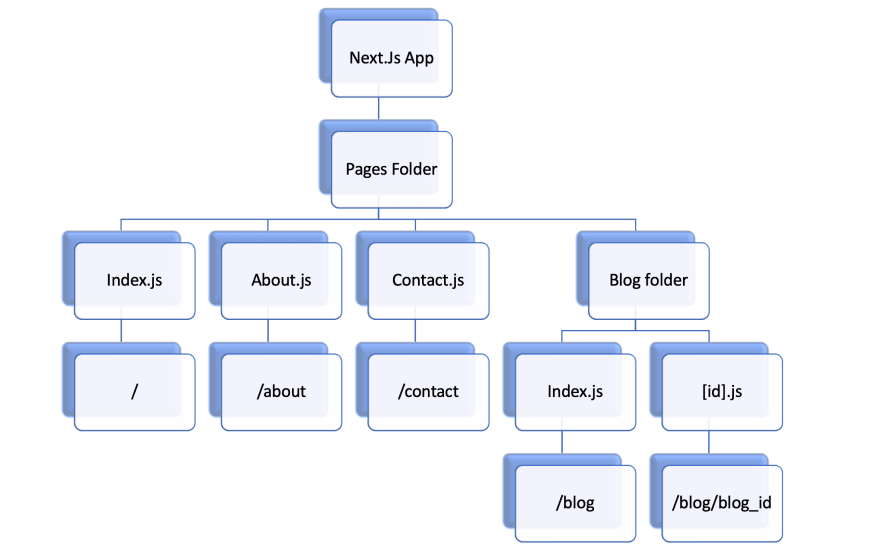
\includegraphics[width=0.5\textwidth]{Nextjs/Routing}
            \caption{Sistema de enrutamiento de Next.js.}
            \label{fig:nextjs_routing}
        \end{figure}
    \end{comment}

    \item \textbf{Pre-rendering}: El HTML para cada página es generado por adelantado, en lugar de que JavaScript en el cliente lo haga todo. Esto resulta en un mejor rendimiento y SEO. Cuando llegue el robot de Google recibirá el contenido ya renderizado, esto permitirá posicionar igual que una web estática. 
    %(Ver figura \ref{fig:Prerendering}).

    \begin{comment}
        \begin{figure}[H]
            \centering
            \subfloat[Sin Pre-rendering.]{
                \label{fig:nextjs_noprerendering}
                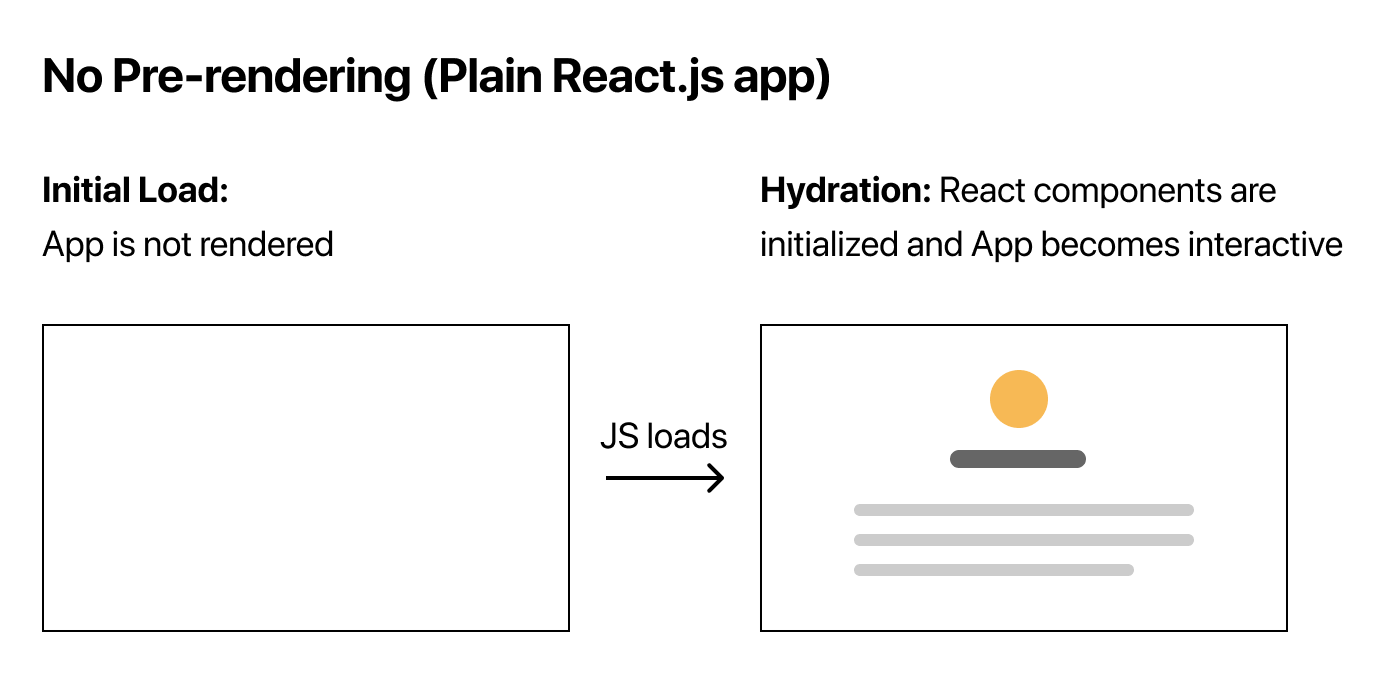
\includegraphics[width=0.45\textwidth]{Nextjs/NoPrerender}}
            \subfloat[Con Pre-rendering.]{
                \label{fig:nextjs_prerendering}
                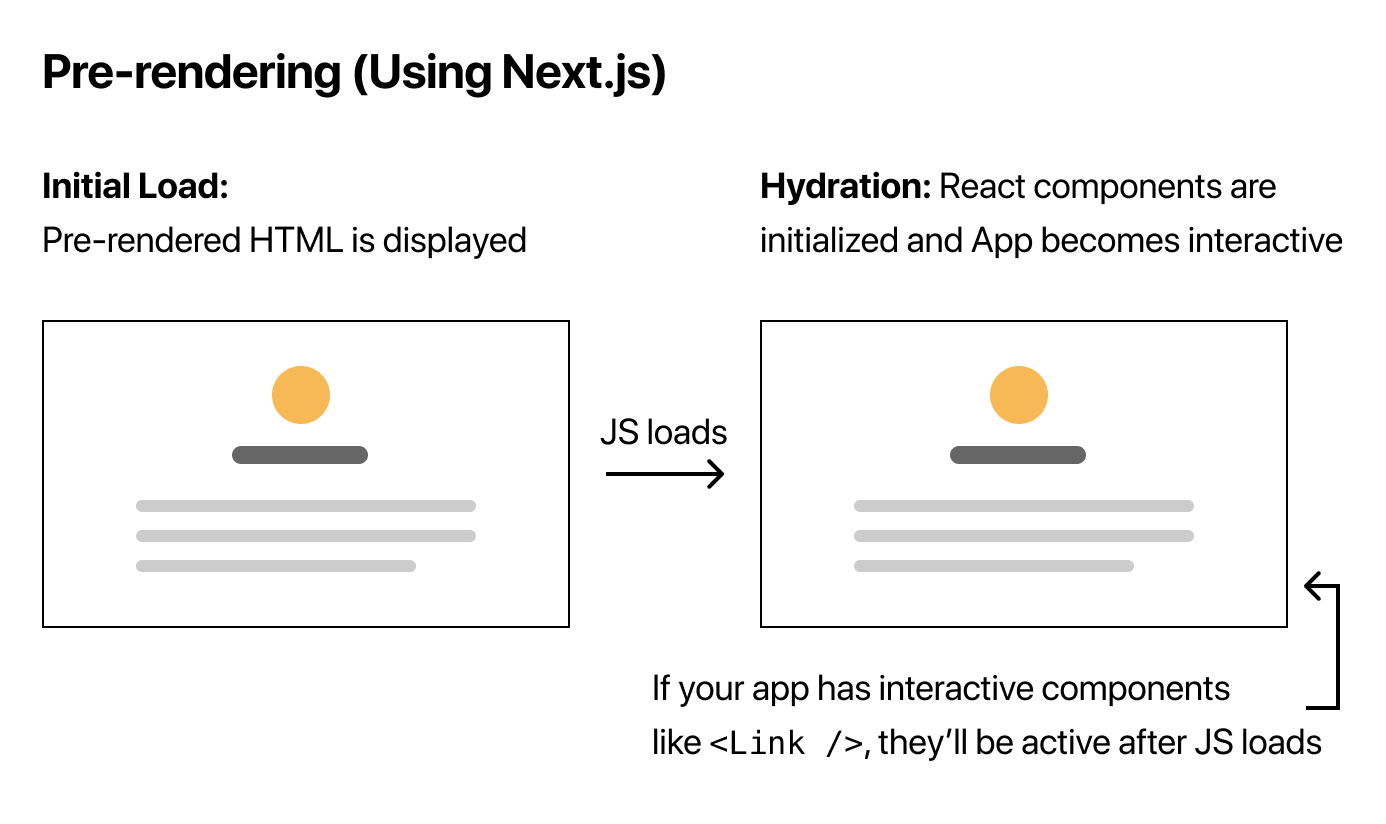
\includegraphics[width=0.45\textwidth]{Nextjs/Prerender}}
            \caption{Prerendering de páginas de Next.js.}
            \label{fig:Prerendering}
       \end{figure}
    \end{comment}

    Next.js tiene dos formas de pre-rendering:
    \begin{itemize}
        \item \textbf{Server-side Rendering:} El HTML se genera en cada solicitud. %(Ver figura \ref{fig:nextjs_ssr}).
        \item \textbf{Generación Estática:} El HTML se genera en el momento de la compilación y se reutilizará en cada solicitud. Esta forma es la utilizada por razones de rendimiento. %(Ver figura \ref{fig:nextjs_ssg})
    \end{itemize}

    \begin{comment}
        \begin{figure}[H]
            \centering
            \subfloat[Server-side Rendering.]{
                \label{fig:nextjs_ssr}
                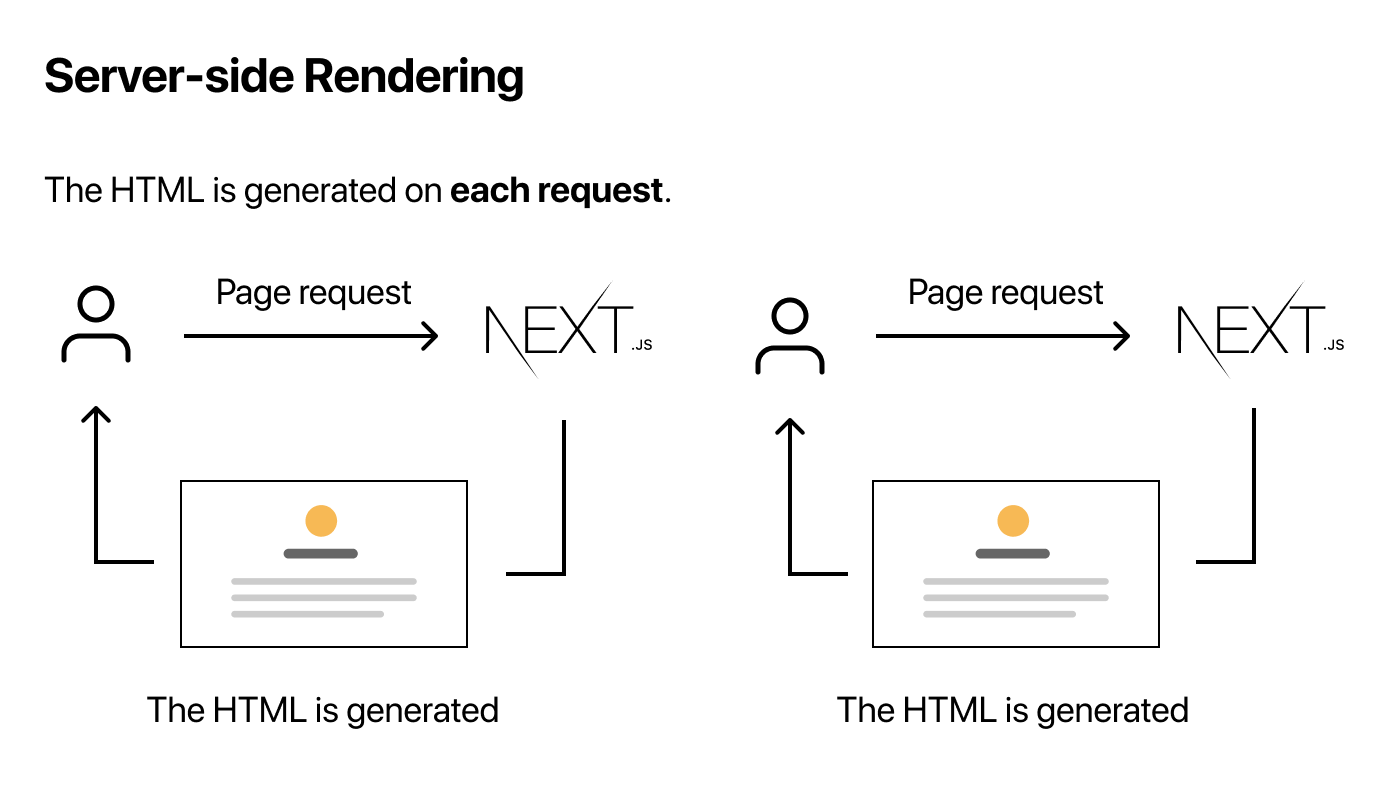
\includegraphics[width=0.45\textwidth]{Nextjs/SSR}}
            \subfloat[Generación Estática.]{
                \label{fig:nextjs_ssg}
                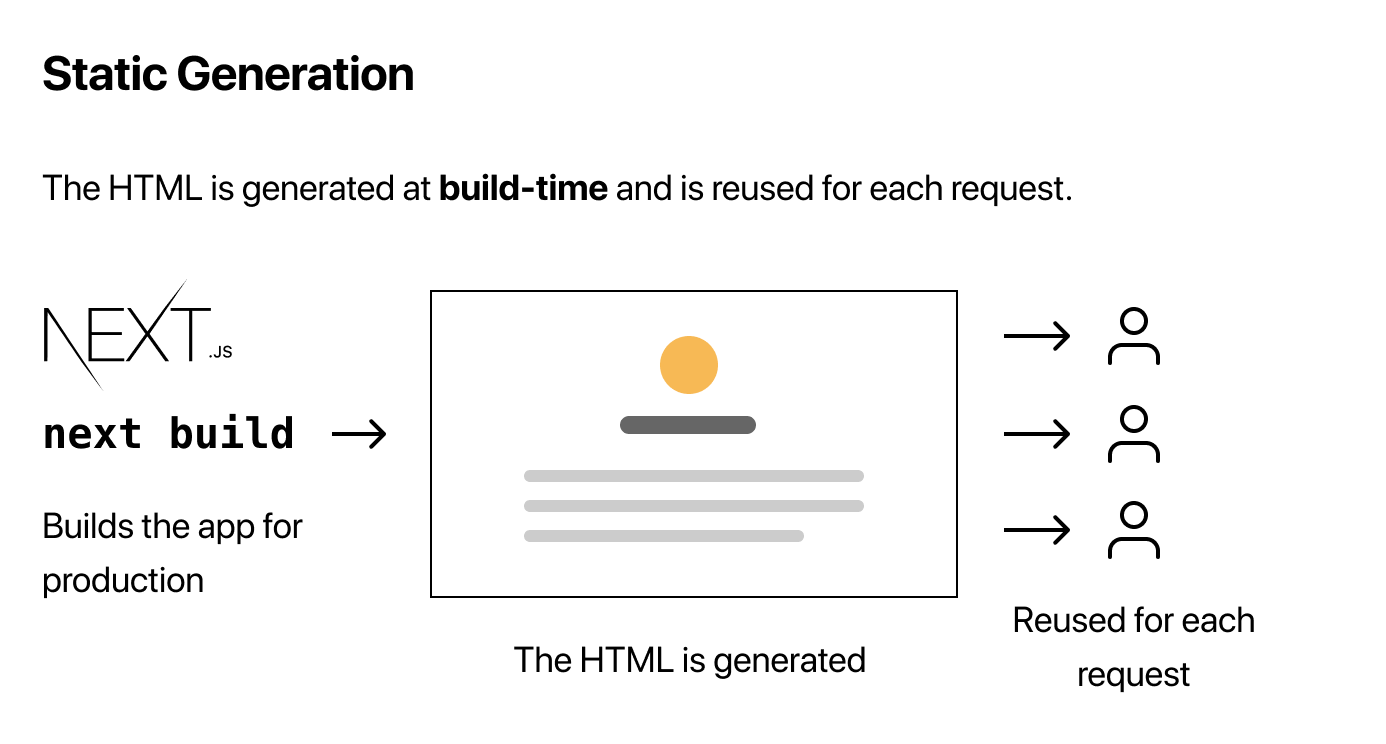
\includegraphics[width=0.45\textwidth]{Nextjs/SSG}}
            \caption{Tipos de Pre-rendering de Next.js.}
            \label{fig:TiposPrerendering}
       \end{figure}
    \end{comment}

    \item \textbf{Code Splitting} para cargas de página más rápidas: La división automática del código en varios paquetes o componentes que luego se pueden cargar a medida y en paralelo. 
    %(Ver figura \ref{fig:codesplit}).
    
    \begin{comment}
        \begin{figure}[H]
            \centering
            \subfloat[Sin Code Splitting.]{
            \label{fig:nextjs_nocodesplit}
            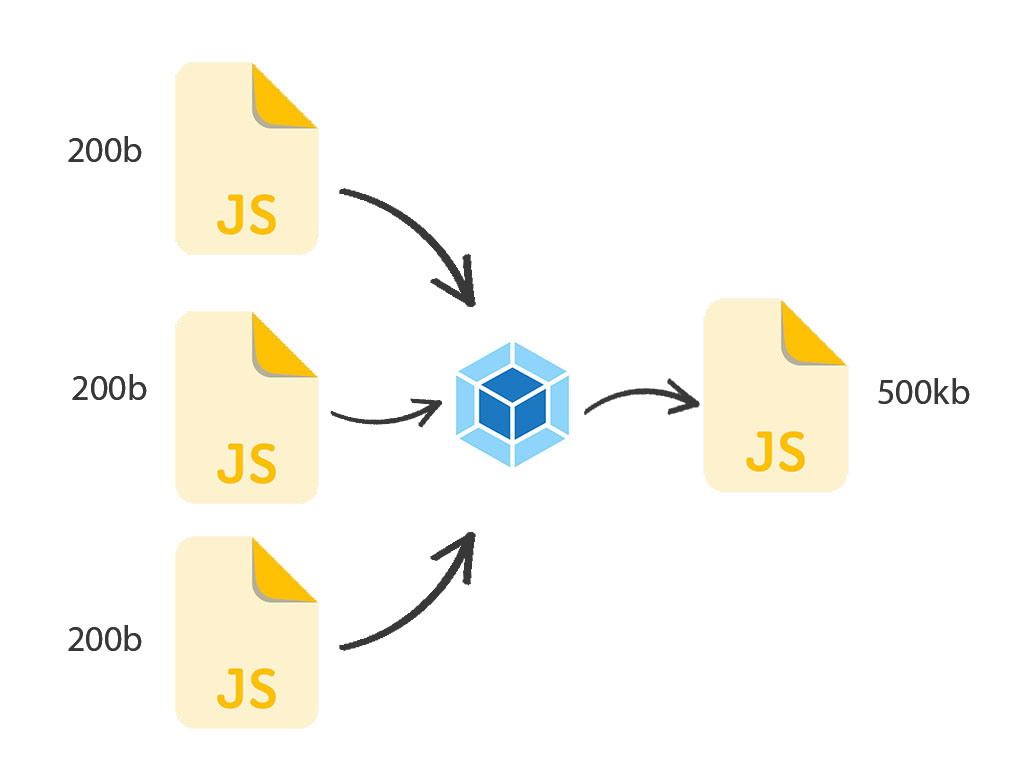
\includegraphics[width=0.35\textwidth]{Nextjs/NoCodeSplit}}
            \subfloat[Con Code Splitting.]{
            \label{fig:nextjs_codesplit}
            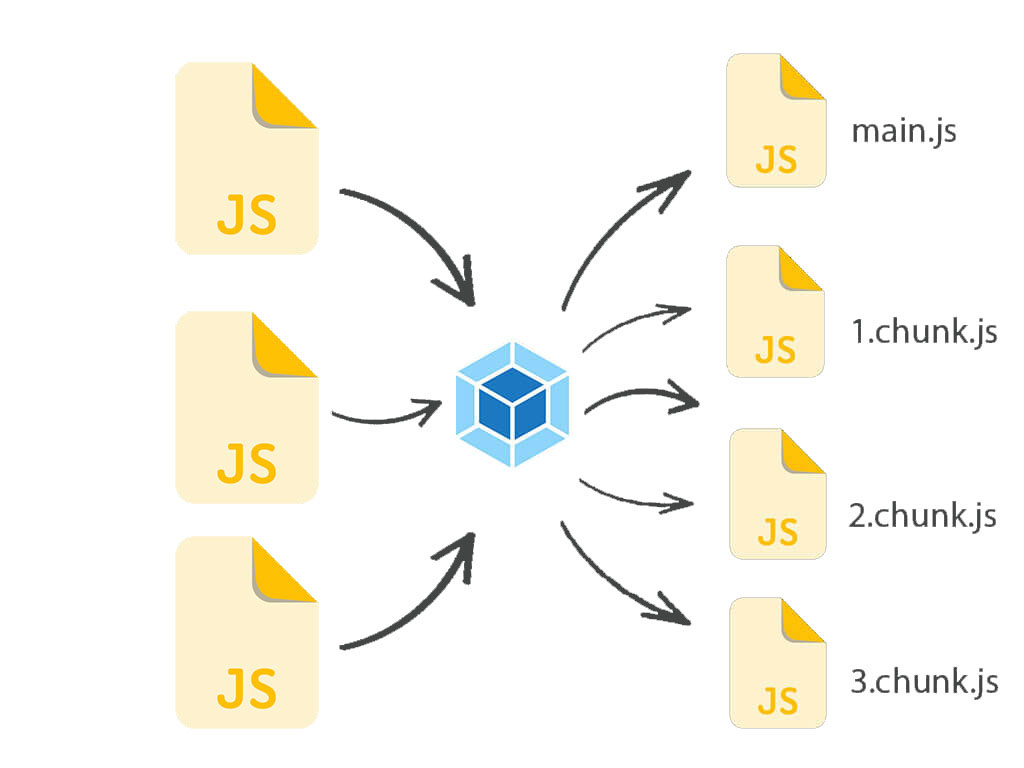
\includegraphics[width=0.35\textwidth]{Nextjs/CodeSplit}}
            \caption{Code Splitting con Next.js y Webpack.}
            \label{fig:codesplit}
        \end{figure}
    \end{comment}

    \item \textbf{Enrutamiento optimizado con prefetching} para SPA: La aplicación precarga los recursos mostrados en la página actual para que su acceso sea mucho más rápido al navegar. 
    %(Ver figura \ref{fig:nextjs_prefetch}).

    \begin{comment}
        \begin{figure}[H]
            \centering
            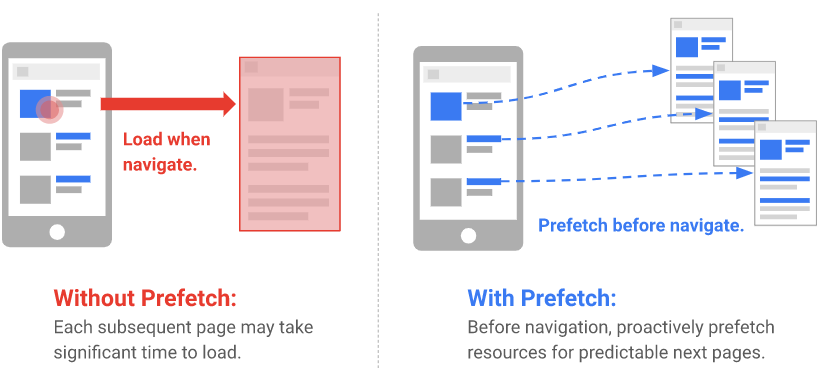
\includegraphics[scale=0.3]{Nextjs/Prefetch}
            \caption{Prefetching de recursos de Next.js.}
            \label{fig:nextjs_prefetch}
        \end{figure}
    \end{comment}

    \item \textbf{Fast Refresh y HMR} (Hot Module Replacement) para el entorno de desarrollo: Permite actualizar todo tipo de módulos y componentes de React en tiempo de ejecución sin necesidad de un refresco completo. Lo que mejora la experiencia y velocidad del desarrollo.
    %(Ver figura \ref{fig:nextjs_hmr}).

    \begin{comment}
        \begin{figure}[H]
            \centering
            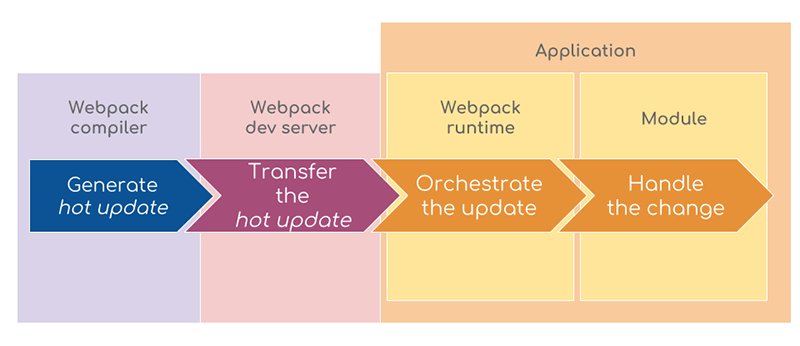
\includegraphics[scale=0.33]{Nextjs/FastRefresh}
            \caption{Fast Refresh de Next.js.}
            \label{fig:nextjs_hmr}
        \end{figure}   
    \end{comment}

    \item \textbf{Soporte integrado de CSS, Sass} y \textbf{CSS-in-JS}: Lo que permite abstraer CSS al nivel del componente, utilizando JavaScript para describir estilos de forma declarativa y mantenible.
    \item \textbf{Rutas API} para crear endpoints con Serverless Functions: Cualquier archivo dentro de la carpeta ``pages/api'' se asigna a ``/api/*'' y se tratará como un endpoint en lugar de una página.
    \item \textbf{Compatible con TypeScript} de forma predeterminada y con tipos integrados para las páginas y la API.
\end{itemize}

%Simplemente instalamos Nextjs, así como TypeScript, React y React-dom como dependencias. Estas dos últimas son necesarias para que Next pueda trabajar sin ningún tipo de problemas.

\subsection{React}
\label{sec:React}

Es una biblioteca de \textbf{JavaScript} mantenida por Facebook, que permite crear interfaces de usuario mediante componentes interactivos y reutilizables \cite{react1}.
%(Ver figura \ref{fig:ReactLogo}).

\begin{comment}
\begin{figure}[H]
    \centering
    
\includegraphics[scale=0.07]{React/React}
    \caption{Logo de React.}
    \label{fig:ReactLogo}
\end{figure}
\end{comment}

%React está basado en un paradigma llamado \textbf{programación orientada a componentes} en el que cada componente es una pieza con la que el usuario puede interactuar. 
Estos componentes se crean usando una sintaxis llamada JSX permitiendo escribir HTML y CSS dentro de objetos JavaScript y se combinan para crear componentes mayores hasta configurar una web completa.

\begin{comment}
    \begin{figure}[H]
        \centering
        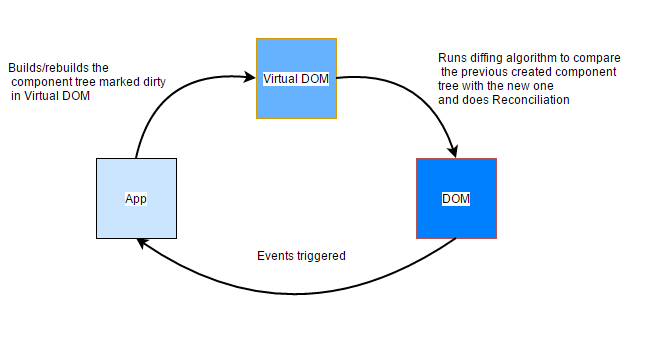
\includegraphics[scale=0.5]{React/VirtualDOM1}
        \caption{Proceso de reconciliación del Virtual DOM de React.}
        \label{fig:React_VirtualDom}
    \end{figure}
\end{comment}

Además, genera el DOM de forma dinámica, hace los cambios en un \textbf{DOM virtual} y después la compara con la versión actual del DOM. Aplica los cambios sólo al componente actualizado, evitando renderizar toda la página. Esto propicia una mejor experiencia de usuario, gran rendimiento y fluidez \cite{react2}.
%(Ver figura \ref{fig:React_VirtualDom}).

\subsection{Vercel}
\label{sec:Vercel}

Es una plataforma en la nube que permite \textbf{alojar sitios web} y servicios web que escalan automáticamente y no requieren supervisión \cite{vercel1}. %(Ver figura \ref{fig:VercelLogo}). 

Proporciona dominios personalizados, variables de entorno, HTTPS automático y una vista previa de cada rama de Github.
Además, desplegar una aplicación \textbf{Next.js} tiene las siguientes ventajas:

\begin{compactitem}
    \item Las páginas que usan generación estática y assets se publican automáticamente desde el \textbf{Vercel Edge Network}, que es increíblemente rápido.
    \item Las páginas que usan pre-rendering y rutas API se convierten en \textbf{Serverless Functions}, permitiendo que el renderizado y las solicitudes puedan escalar.
\end{compactitem}

\begin{comment}
    \begin{figure}[H]
        \centering
        
\includegraphics[scale=0.5]{Vercel/Vercel}
        \caption{Logo de Vercel.}
        \label{fig:VercelLogo}
    \end{figure}
\end{comment}

Por último, ofrece \textbf{Vercel Analytics} para medir el rendimiento de la web, recopilando las web vitals de los dispositivos reales que utilizan los usuarios \cite{vercelAnalytics}.

\subsection{TypeScript}
\label{sec:TypeScript}

Es un lenguaje de programación desarrollado y mantenido por Microsoft. Es un superconjunto de \textbf{JavaScript}, que añade \textbf{tipos estáticos} y objetos basados en clases \cite{typescript}.
%(Ver figura \ref{fig:TypeScriptLogo}).

\begin{comment}
    \begin{figure}[H]
        \centering
        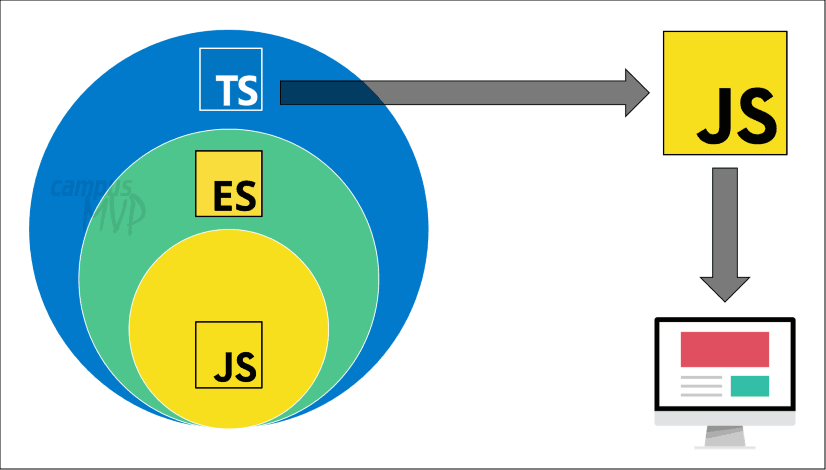
\includegraphics[scale=0.03]{TypeScript/TypeScript}
        \caption{Logo de TypeScript.}
        \label{fig:TypeScriptLogo}
    \end{figure}
\end{comment}

%Como es un superconjunto de JavaScript, todo el código escrito en JavaScript es válido para TypeScript. Pero lo contrario no es cierto. Es decir, como los navegadores no entienden TypeScript, es necesario transpilarlo a JavaScript antes de usarlo en un navegador. Al crear nuestra aplicación con \textbf{Nextjs} ya obtenemos transpilación y empaquetado automáticos con \textbf{SWC} y \textbf{Webpack} respectivamente.
%(ver figura \ref{fig:TypeScript})

\begin{comment}
    \begin{figure}[H]
        \centering
        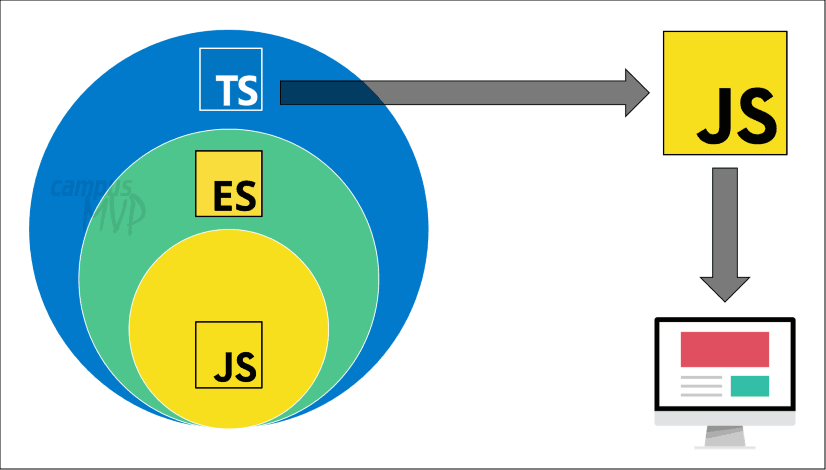
\includegraphics[scale=0.35]{TypeScript/TypeScriptTranspile}
        \caption{Diagrama de transpilación de TypeScript a JavaScript.}
        \label{fig:TypeScript}
    \end{figure}
\end{comment}

Es un lenguaje más limpio, robusto y mantenible. Permite escribir código con menos errores, más sencillo, coherente y fácil de probar. Además, ayuda a implementar patrones de diseño e incrementa la agilidad en el refactoring.

Los navegadores no entienden TypeScript, por lo que es necesario transpilarlo a JavaScript antes de usarlo. Al crear nuestra aplicación con \textbf{Nextjs} ya obtenemos transpilación y empaquetado automáticos con \textbf{SWC} y \textbf{Webpack}.
\cite{typescript2}

\subsection{Node.js}
\label{sec:Node}

Es un entorno de tiempo de ejecución de \textbf{JavaScript}. Orientado a eventos asíncronos, incluye todo lo necesario para ejecutar un programa JavaScript \cite{node}.
%(Ver figura \ref{fig:NodejsLogo}).

\begin{comment}
    \begin{figure}[H]
        \centering
        
\includegraphics[scale=0.4]{Nodejs/Nodejs}
        \caption{Logo de Node.js.}
        \label{fig:NodejsLogo}
    \end{figure}
\end{comment}

Permite utilizar un único lenguaje para el Backend y el FrontEnd. Además, cuenta con un repositorio de código abierto lleno de \textbf{librerías} útiles. %, lo que ayuda a una generación rápida de un producto mínimo viable.

Debe estar instalado con \textbf{NPM} o \textbf{Yarn}, dos gestores de paquetes para proyectos de Node.js \cite{npm}. A veces, la \textbf{instalación de paquetes} con NPM no es lo suficiente consistente o rápida, dando incluso errores. Este es el motivo para usar Yarn, una alternativa construida por Facebook, Google, Exponent y Tilde \cite{yarn}\cite{npmyarn}.

\begin{comment}
\subsubsection{NPM vs. Yarn}
A veces, la \textbf{instalación de paquetes} con NPM no es lo suficiente consistente o rápida, dando incluso errores. Este es el motivo para usar Yarn, una alternativa construida por Facebook, Google, Exponent y Tilde \cite{npmyarn}.
(Ver figura \ref{fig:NPMYarnLogo}).
    \begin{figure}[H]
        \centering
        
\includegraphics[scale=0.4]{Nodejs/NPMvsYarn}
        \caption{Logo de NPM y Yarn.}
        \label{fig:NPMYarnLogo}
    \end{figure}
Una diferencia es que en el \textbf{package.json}, el archivo donde se hace un seguimiento de las dependencias del proyecto, los números de versión no siempre son exactos. En su lugar, se puede definir una gama de versiones.
Cada vez que se añade un módulo, Yarn crea o actualiza un archivo \textbf{yarn.lock}.
De esta manera se puede garantizar que se vuelva a instalar exactamente el mismo paquete, sin dejar de tener una gama de versiones permitidas en package.json. 
\end{comment}

\subsection{VSCode}
\label{sec:VSCode}

Es un \textbf{editor de código} optimizado para crear aplicaciones modernas. Incluye depuración, control integrado de Git, resaltado de sintaxis, finalización inteligente y refactorización de código \cite{vscode}.
%(Ver figura \ref{fig:VSCodeLogo}).

\begin{comment}
    \begin{figure}[H]
        \centering
        \includegraphics[scale=0.035]{VSCode/VSCode}
        \caption{Logo de VSCode.}
        \label{fig:VSCodeLogo}
    \end{figure}
\end{comment}

%Gracias a su \textbf{integración de Git} es sencillo revisar las diferencias, preparar los archivos y realizar confirmaciones directamente desde el editor antes de subirlo al repositorio en la nube.

Además, cuenta con una biblioteca de \textbf{extensiones} para ser más eficiente programando. Desde extensiones de lenguajes de programación hasta herramientas para visualizar o estructurar el código.

Las extensiones más importantes para mejorar la experiencia de desarrollo y buenas prácticas de este proyecto fueron \textbf{ESLint} y \textbf{Prettier}. Configurar estas herramientas es una inversión que se hace una vez y sus beneficios notan durante todo el desarrollo.

\subsubsection{ESLint}

Es una herramienta de \textbf{análisis de código} para identificar patrones problemáticos que se puede instalar como extensión en VSCode \cite{eslint}.
%(Ver figura \ref{fig:ESLintLogo}).

\begin{comment}
    \begin{figure}[H]
        \centering
        
\includegraphics[scale=0.05]{VSCode/ESLint}
        \caption{Logo de ESLint.}
        \label{fig:ESLintLogo}
    \end{figure}
\end{comment}

Su función es analizar el código, detectar problemas y si puede:

\begin{compactitem}
 \item Corregir errores de sintaxis.
 \item Corregir código poco intuitivo o difícil de mantener.
 \item Evitar el uso de ``malas prácticas''.
 \item Hacer uso de un estilo de código consistente.
\end{compactitem}

Está diseñado para ser flexible y configurable por lo que añadimos ejecutarlo como parte del proceso de integración continua. 
Se pueden usar guías de estilo cómo Airbnb, Standard o Google. En este caso la configuración es la \textbf{guía de estilo} recomendada de ESLint con reglas para TypeScript y React. 

\subsubsection{Prettier}

Es una herramienta para \textbf{formatear el código} que se puede instalar como extensión en VSCode \cite{prettier}. 

Su función es analizar el código y aplicar un estilo consistente, dando formato según sus propias reglas a cosas como: 
%(Ver figura \ref{fig:PrettierLogo}).

\begin{compactitem}
    \item La longitud máxima de línea.
    \item El tipo de identación.
    \item Los saltos de línea.
    \item El orden de los imports.
   \end{compactitem}

\begin{comment}
\begin{figure}[H]
    \centering
    
\includegraphics[scale=0.02]{VSCode/Prettier}
    \caption{Logo de Prettier.}
    \label{fig:PrettierLogo}
\end{figure}
\end{comment}

Su objetivo es acabar con los debates sobre el \textbf{estilo del código}. Para ello, analiza el código y lo da formato cada vez que se guarda el archivo. Para usarlo junto con ESLint hay que configurar este último para que use Prettier.

En definitiva, Prettier se usa para problemas de formato de código y ESLint para problemas de calidad de código.

\section{Detalles de Implementación}
\label{sec:implementacion}

La principal documentación con la que contamos es el estilo de nomenclatura, la coherencia a la hora de nombrar cosas y una arquitectura general coherente. Esta debe emanar de una serie de patrones que se repiten a lo largo del proyecto, tanto a nivel arquitectónico como de diseño. Esta información reside en el código: en el nombre de los componentes, de las variables y de las funciones. Este código se puede encontrar en el siguiente \textbf{repositorio de Github}: 
%(ver figura \ref{fig:GitHubLogo}):

\url{https://github.com/alberttogoca/EarFit}.

\begin{comment}
\begin{figure}[H]
    \centering
    \includegraphics[scale=0.03]{Detalles de Implementación/GitHub}
    \caption{Logo de GitHub.}
    \label{fig:GitHubLogo}
\end{figure}
\end{comment}

Para dejar reflejados estos detalles en la memoria se explicarán todas las partes de las que se compone esta implementación:
\begin{compactitem} 
\item \hyperref[sec:arquitectura]{\textbf{Arquitectura}}. 
\item \hyperref[sec:archivos]{\textbf{Estructura de Archivos}}.
\item \hyperref[sec:tipos]{\textbf{Tipos}}.
\item \hyperref[sec:lib]{\textbf{Librerías}}.
\item \hyperref[sec:servicios]{\textbf{Servicios}}.
\item \hyperref[sec:Hooks]{\textbf{Hooks}}.
\item \hyperref[sec:componentes]{\textbf{Componentes}}.
\end{compactitem} 

No hará falta estar familiarizado con los conceptos propios de React para haber entendido está documentación al acabar.

\subsection{Arquitectura}
\label{sec:arquitectura}

La arquitectura indica la \textbf{estructura, funcionamiento e interacción} entre las diferentes partes de las que esta compuesto el software. En este diagrama se muestra el diseño de más alto nivel de la estructura del sistema (ver figura \ref{fig:Arquitectura}).

\begin{figure}[H]
    \centering
    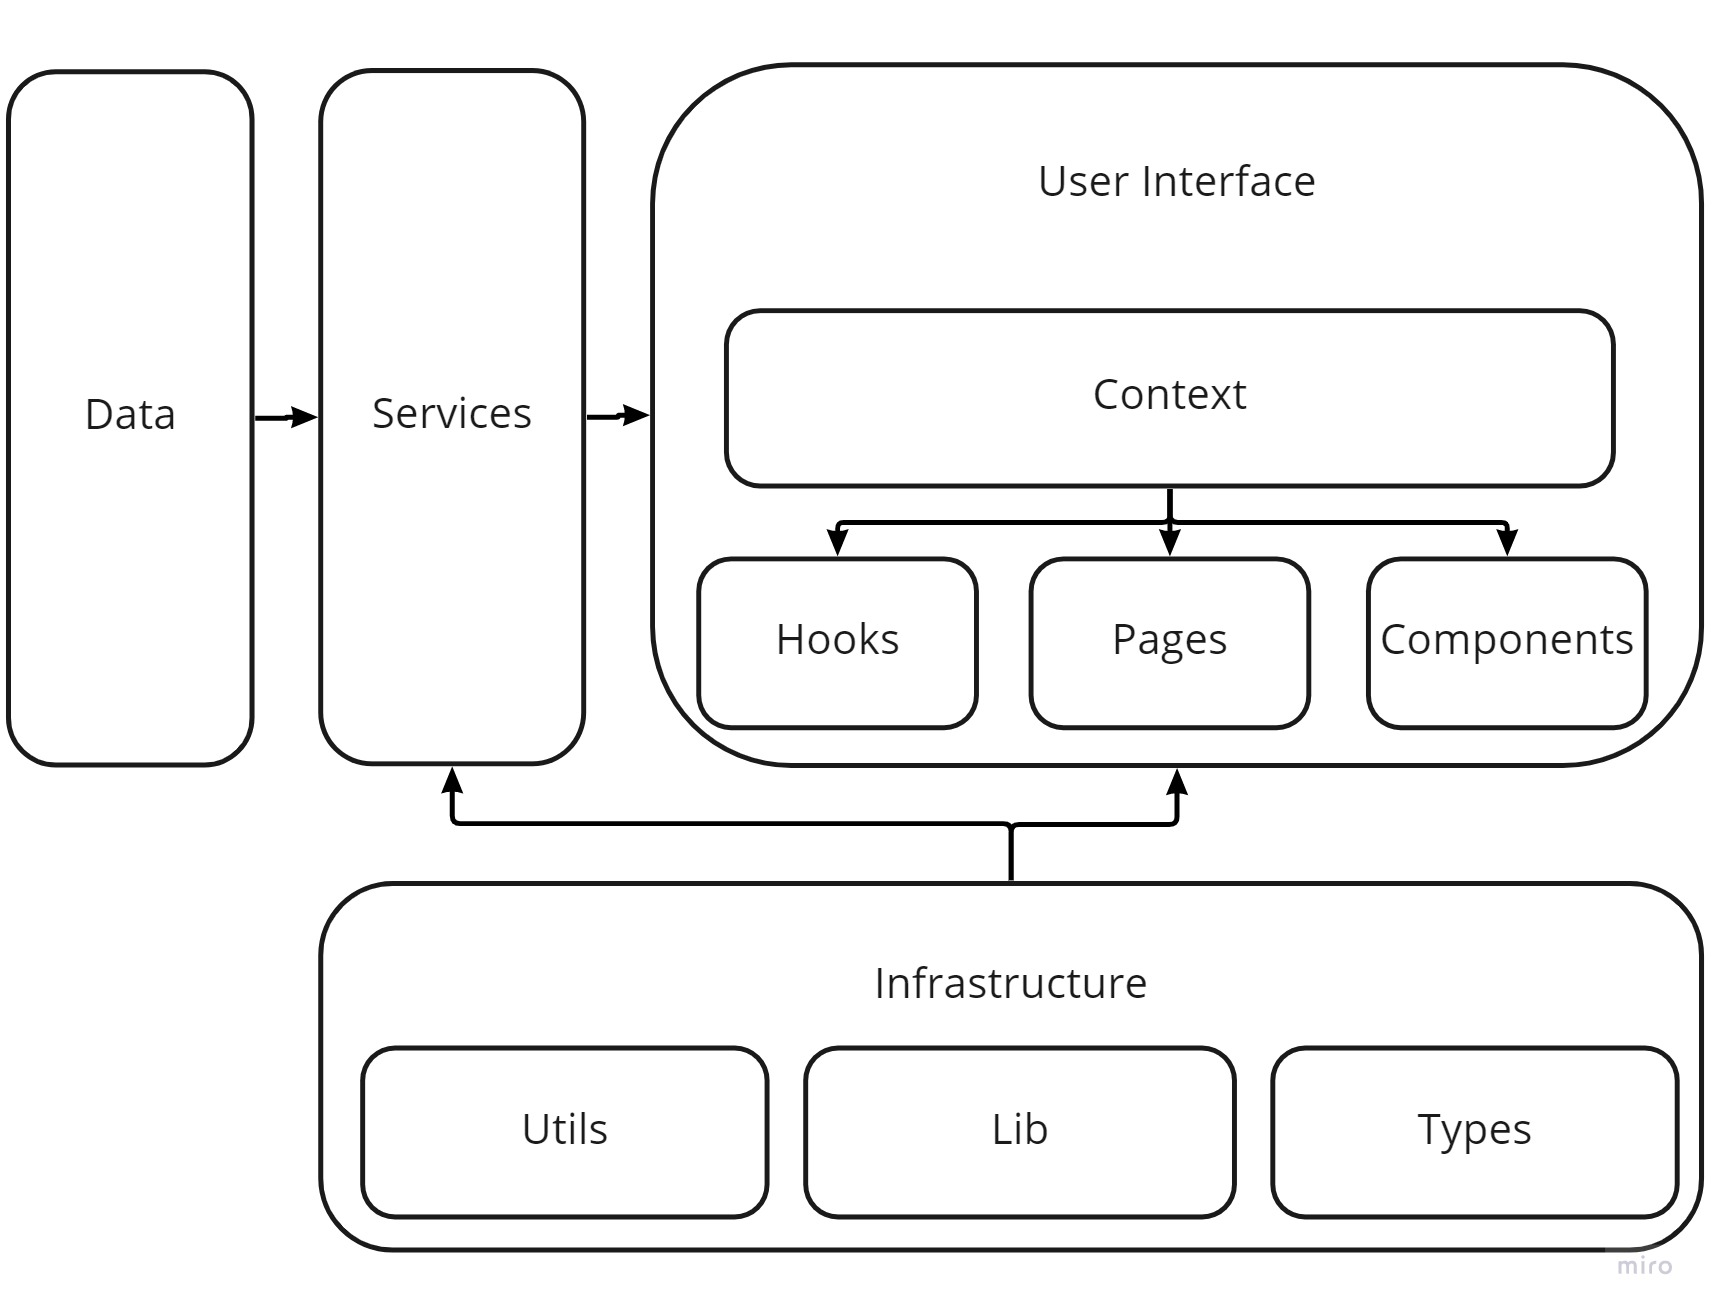
\includegraphics[width=0.85\textwidth]{Detalles de Implementación/Arquitectura}
    \caption{Arquitectura de la aplicación.}
    \label{fig:Arquitectura}
\end{figure}

Esta arquitectura esta formada por \textbf{varias capas desacopladas}: infraestructura, datos, servicios e interfaz de usuario. Estas capas interactúan entre sí de la siguiente manera:

\begin{itemize}
    \item \textbf{La infraestructura} se compone de funciones, librerías y tipos de Typescript que apoyan la lógica de los servicios y de la interfaz.
    \item \textbf{Los servicios} proveen los datos y alguna lógica independiente a la capa de interfaz de usuario.
    \item \textbf{El contexto y los Hooks} usan los servicios y se hacen cargo de crear y manejar los estados necesarios para los componentes.
    \item \textbf{Las páginas y los componentes} hacen uso del contexto y los Hooks, y renderizan la interfaz de usuario.
\end{itemize}

\subsection{Estructura de Archivos}
\label{sec:archivos}

%React no tiene opiniones sobre cómo estructurar los archivos \cite{reactArchivos}. 
\textbf{Nextjs} tiene algunos archivos y \textbf{directorios especiales} \cite{reactArchivos}. Como mínimo, se necesita una carpeta ``pages'' con un archivo ``index.js''. Además, la carpeta ``public'' tiene una función específica. Aparte de estos archivos y directorios, todo vale \cite{nextjs2}.

En este caso se han separado las \textbf{carpetas por conceptos} o intereses (Ver figura \ref{fig:Archivos}). Cada carpeta contiene archivos similares siguiendo la arquitectura:

\begin{figure}[H]
    \centering
    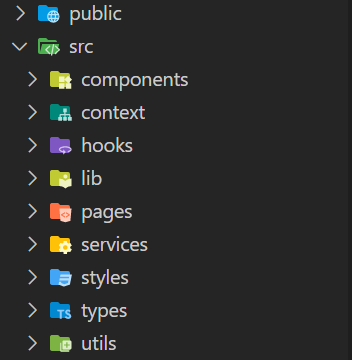
\includegraphics[width=0.45\textwidth]{Detalles de Implementación/Estructura de Archivos/Archivos}
    \caption{Estructura de Archivos.}
    \label{fig:Archivos}
\end{figure}

\begin{itemize}
    \item \href{https://github.com/alberttogoca/EarFit/tree/main/src/pages}{\textbf{Pages}}: Aquí se encuentran todas las páginas de la aplicación. Cada página está asociada con una ruta basada en su nombre de archivo. Por ejemplo: en ``pages/notes'' se exporta un componente de React que será accesible en la URL ``/notes''.
    
    El archivo ``index.js'' es la página que se representa cuando el usuario visita la ruta raíz de la aplicación.

    Aparte, para tener un Layout persistente está el archivo ``\_app.tsx''. En este archivo se encuentran los metadatos de la aplicación y se envuelve la aplicación con el Layout. 
    
    Por otro lado, en el archivo ``\_document.tsx'' se actualizan las etiquetas ``\texttt{<html>}'' y ``\texttt{<body>}''.
    \item \href{https://github.com/alberttogoca/EarFit/tree/main/public}{\textbf{Public}}: Aquí se encuentran los iconos, imágenes, Service Worker, Manifest y archivos fuente de sonido en formato MIDI.js. En Next.js el código puede hacer referencia a los archivos estáticos dentro de una ``public'' en el directorio raíz a partir de la URL base (/).
    \item \href{https://github.com/alberttogoca/EarFit/tree/main/src/components}{\textbf{Components}}: Aquí se encuentran todos los componentes de la aplicación agrupados por carpetas. El modelo React nos permite deconstruir una página en una serie de componentes. Muchos de estos componentes a menudo se reutilizan entre páginas.
    \item \href{https://github.com/alberttogoca/EarFit/tree/main/src/context}{\textbf{Context}}: Aquí se encuentra el contexto de la aplicación. El Context está diseñado para compartir estados que pueden considerarse “globales” para un árbol de componentes en React. %Como es un componente especial, como las pages, tiene su propio directorio.
    \item \href{https://github.com/alberttogoca/EarFit/tree/main/src/hooks}{\textbf{Hooks}}: Aquí se encuentran todos los Custom Hooks creados para extraer la lógica de los componentes en funciones reutilizables. Los Hooks son una nueva característica en React 16.8. Estos permiten usar el estado y otras características de React sin escribir una clase.
    \item \href{https://github.com/alberttogoca/EarFit/tree/main/src/lib}{\textbf{Lib}}: Aquí se encuentra ``soundfont-wrapper'', una librería personalizada para la aplicación. Para hacer uso de la librería ``soundfont-player'', que se encarga de cargar los archivos fuente de sonido y usarlos mediante la Web Audio API. Se creó esta librería envoltorio (wrapper library) para refinar la complejidad de su interfaz y simplificar su uso.
    \item \href{https://github.com/alberttogoca/EarFit/tree/main/src/services}{\textbf{Services}}: Aquí se encuentran los servicios que serán consumidos desde los Hooks. Los servicios proporcionan los datos y un conjunto de métodos responsables de alguna lógica específica independiente a la interfaz.
    \item \href{https://github.com/alberttogoca/EarFit/tree/main/src/styles}{\textbf{Styles}}: Aquí se encuentran algunos estilos css globales. Aunque en general se hace uso de ``react-bootstrap'' junto con ``bootswatch'' para los estilos de la aplicación.
    \item \href{https://github.com/alberttogoca/EarFit/tree/main/src/types}{\textbf{Types}}: Aquí se encuentran todos los tipos usados en los demás archivos de la aplicación. Para usar Typescript todos los archivos ``.js'' se convierten en ``.ts'' y ``.jsx'' en ``.tsx''.
    \item \href{https://github.com/alberttogoca/EarFit/tree/main/src/utils}{\textbf{Utils}}: Aquí encuentran los archivos con métodos genéricos para ser usados en cualquier parte de la aplicación.
\end{itemize}

Por otro lado, en el directorio raíz del proyecto se encuentran los archivos de configuración: ``.eslintrc.js'', ``.gitignore'', ``.prettier.js'', ``next-env.d.ts'', ``next.config.js'', ``tsconfig.json'', ``package.json'' y ``yarn.lock''. 
Y por último, también se encuentra un archivo ``README.md'' con una breve presentación y explicación de la aplicación.

\subsection{Infraestructura}

\subsubsection{Tipos}
\label{sec:tipos}

A continuación, se explican los tipos de \textbf{Typescript} creados para la implementación. Estos tipos son una manera de documentar el código y evitar errores que Javascript no proporciona. Ayudan a leer y entender el código de una forma más efectiva.

\begin{itemize}
    \begin{figure}[H]
        \centering
        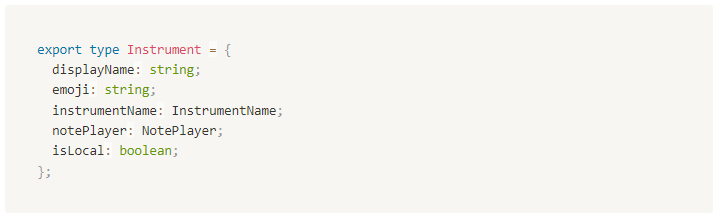
\includegraphics[scale=0.6]{Detalles de Implementación/Code/Types/Instrument}
        \caption{Tipo Instrument.}
        \label{fig:Instrument}
    \end{figure}

    \item \href{https://github.com/alberttogoca/EarFit/blob/main/src/types/index.ts}{\textbf{Instrument}}: Este tipo define a los instrumentos en la aplicación. Cada instrumento tiene un nombre, un emoji, un nombre identificador del instrumento, un ``notePlayer'' para tocar notas y un booleano que especifica si se tiene el archivo de sonido en una carpeta local. (Ver figura \ref{fig:Instrument}).
    \item \href{https://github.com/alberttogoca/EarFit/blob/main/src/types/index.ts}{\textbf{InstrumentName}}: Este tipo define el nombre identificador del instrumento. Esta definido por la librería ``Soundfont-player-js'' como una lista de instrumentos disponibles. Sirve para buscar el archivo MIDI de dicho instrumento y crear su ``notePlayer''. %Si un instrumento no está en esta lista, significa que no existe su archivo MIDI en el repositorio fuente de la librería, pero se podría tener este archivo en local.
    
    \begin{figure}[H]
        \centering
        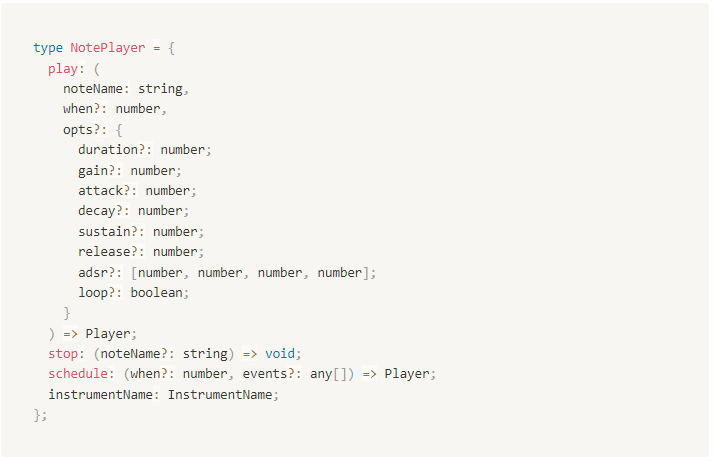
\includegraphics[scale=0.6]{Detalles de Implementación/Code/Types/Noteplayer}
        \caption{Tipo Noteplayer.}
        \label{fig:Noteplayer}
    \end{figure}

    \item \href{https://github.com/alberttogoca/EarFit/blob/main/src/types/index.ts}{\textbf{Noteplayer}}: Este tipo proporciona funciones para reproducir los sonidos de dicho instrumento. Este tipo es proporcionado por la librería ``Soundfont-wrapper''. (Ver figura \ref{fig:Noteplayer}).

    \begin{figure}[H]
        \centering
        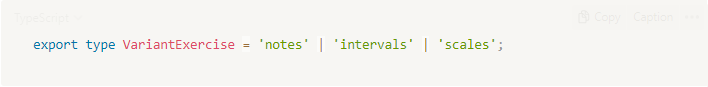
\includegraphics[scale=0.6]{Detalles de Implementación/Code/Types/VariantExercise}
        \caption{Tipo VariantExercise.}
        \label{fig:VariantExercise}
    \end{figure}

    \item \href{https://github.com/alberttogoca/EarFit/blob/main/src/types/index.ts}{\textbf{VariantExercise}}: Este tipo define la tres variantes del ejercicio: ``notes'', ``intervals'' y ``scales''. En la aplicación se tratan todas las páginas de ejercicio como variantes del mismo. Es decir, todas son el mismo ejercicio pero con valores distintos. Lo que nos permite reutilizar toda la lógica como veremos en los Hooks.
    (Ver figura \ref{fig:VariantExercise}).

    \begin{figure}[H]
        \centering
        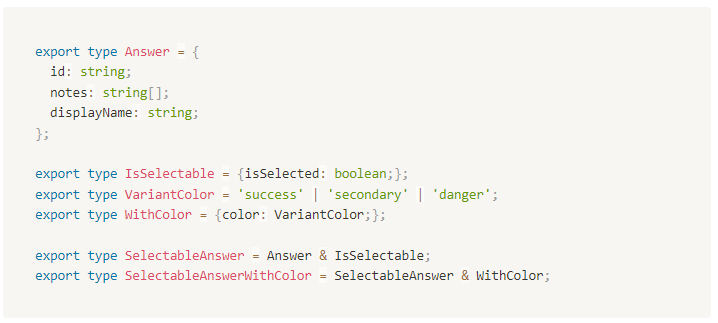
\includegraphics[scale=0.6]{Detalles de Implementación/Code/Types/Answer}
        \caption{Tipo Answer.}
        \label{fig:Answer}
    \end{figure}

    Cada variante de ejercicio utiliza los tipos Answer, SelectableAnswer y SelectableAnswerWithColor. (Ver figura \ref{fig:Answer}).

    \item \href{https://github.com/alberttogoca/EarFit/blob/main/src/types/index.ts}{\textbf{Answer}}: Este tipo define a una respuesta del ejercicio. Cada respuesta tiene un id, un nombre para mostrar y un array de notas para ser reproducidas. Es el tipo base del ejercicio.
    \item \href{https://github.com/alberttogoca/EarFit/blob/main/src/types/index.ts}{\textbf{SelectableAnswer}}: Este tipo añade propiedades por intersección al tipo Answer, necesarias para implementar los botones de selección renderizados por el componente ``AnswerToggles''. La propiedad ``isSelected'' especifica si la respuesta está disponible para preguntar.
    \item \href{https://github.com/alberttogoca/EarFit/blob/main/src/types/index.ts}{\textbf{SelectableAnswerWithColor}}: Este tipo añade propiedades por intersección al tipo SelectableAnswer, necesarias para implementar los botones de respuesta renderizados por el componente ``AnswerButtons''. La propiedad ``color'' especifica el color que debe tomar el botón de respuesta.

    \begin{comment}
        \begin{figure}[H]
            \centering
            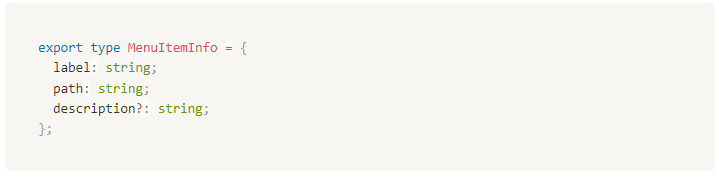
\includegraphics[scale=0.6]{Detalles de Implementación/Code/Types/MenuItemInfo}
            \caption{Tipo MenuItemInfo.}
            \label{fig:MenuItemInfo}
        \end{figure}

        \item \href{https://github.com/alberttogoca/EarFit/blob/main/src/types/index.ts}{\textbf{MenuItemInfo}}: Este tipo define la información necesaria para cada ítem del componente menú. (Ver figura \ref{fig:MenuItemInfo}).
    \end{comment}

\end{itemize}

\subsubsection{Librerías}
\label{sec:lib}

A continuación, se explican los paquetes de \textbf{Node.js} o librerías usadas en la implementación. Todas estas librerías se pueden encontrar definidas con sus versiones en el archivo ``package.json'' o en la carpeta ``lib'' en el caso de ``soundfont-wrapper''.

\begin{itemize}
    \item \href{https://github.com/tonaljs/tonal}{\textbf{Tonaljs}}: Es una librería de teoría musical. Contiene funciones para manipular elementos musicales como notas, intervalos y escalas. Se tratan de abstracciones, no de música o sonido reales \cite{tonal}.
    \item \href{https://github.com/danigb/soundfont-player}{\textbf{Soundfont-player}}: Sirve para cargar archivos MIDI.js y reproducir sonidos utilizando la WebAudio API \cite{webAudioAPI}. Estos archivos contienen los sonidos de los instrumentos codificados. No hace falta contar con estos archivos en local ya que en tal caso los buscaría en el siguiente repositorio: \href{https://github.com/gleitz/midi-js-soundfonts}{{\textbf{midi-js-soundfonts}}} \cite{soundfont-player}.
    \item \href{https://github.com/alberttogoca/EarFit/blob/main/src/lib/soundfont-wrapper.ts}{\textbf{Soundfont-wrapper}}: Es una librería personalizada para refinar la complejidad de ``soundfont-player'' y simplificar su uso. Proporciona la función ``getSoundfontInstrument'' que devuelve un ``notePlayer'' con funciones para tocar notas. Se encarga de crear el ``audioContext'' y gestionar los nodos de audio.
    \item \href{https://github.com/kevinsqi/react-piano}{\textbf{React-piano}}: Proporciona un teclado de piano interactivo para React. No implementa la reproducción de audio de cada nota, por lo que se debe implementar aparte y pasar por Props dos funciones: playNote y stopNote \cite{react-piano}.
    \item \href{https://github.com/pmndrs/react-use-measure}{\textbf{React-use-measure}}: Se usa para conseguir que ``react-piano'' sea responsivo. Lo que hace es obtener la referencia de ancho del componente padre para usarla en el renderizado del piano \cite{react-use-measure}.
    \item \href{https://github.com/react-bootstrap/react-bootstrap}{\textbf{React-bootstrap}}: Es la librería de estilos CSS usada. Cada componente de React-Bootstrap es un verdadero componente de React, sin dependencias innecesarias como jQuery \cite{react-bootstrap}.
    \item \href{https://github.com/shadowwalker/next-pwa}{\textbf{Next-pwa}}: Es un plugin que permite registrar y generar un Service Worker para convertir una aplicación web en una aplicación web progresiva \cite{next-pwa}.
\end{itemize}

\subsubsection{Utils}
En el archivo \href{https://github.com/alberttogoca/EarFit/blob/main/src/utils/arrayUtils.ts}{\textbf{``arrayUtils.ts''}} está el método ``getRandomItem'' que recibe un array y devuelve un elemento al azar. Usado en el Hook ``useAnswer'' para seleccionar la respuesta para el ejercicio. El objetivo era ir añadiendo aquí todas funciones complementarias que se fuesen necesitando. Al final resultó ser una.

\subsection{Datos y Servicios}
\label{sec:datos}
\label{sec:servicios}

A continuación, se explican los servicios creados para la aplicación. Por comodidad y tamaño, los datos que proporcionan los servicios se encuentran en su mismo archivo. Ahorrándonos los pertinentes imports y ganando sencillez a la hora de leer el código.
\begin{comment}
    (Ver figura \ref{fig:Services}).

    \begin{figure}[H]
        \centering
        \includegraphics[scale=0.6]{Detalles de Implementación/Estructura de Archivos/Services}
        \caption{Servicios de la aplicación.}
        \label{fig:Services}
    \end{figure}
\end{comment}

\begin{itemize}
    \item \href{https://github.com/alberttogoca/EarFit/blob/main/src/services/instrumentService.ts}{\textbf{instrumentService.ts}}: Este servicio provee una función ``getInstruments'' que devuelve un array de instrumentos de tipo ``Instrument\text{[]}''. Usa la librería ``soundfont-wrapper'' para obtener los ``notePlayer'' para cada instrumento definido en la constante ``InstrumentData''. De tal manera que añadir o quitar un instrumento es tan sencillo como añadirlo a ``InstrumentData''.
    \item \href{https://github.com/alberttogoca/EarFit/blob/main/src/services/noteService.ts}{\textbf{noteService.ts}}: Este servicio provee una función ``getNotes'' que recibe una escala de tipo ``string'' y devuelve un array de respuestas de tipo ``Answer\text{[]}'' correspondiente a la variante de ejercicio ``notes''. Utiliza la librería Tonal para obtener las notas según la escala.
    \item \href{https://github.com/alberttogoca/EarFit/blob/main/src/services/intervalService.ts}{\textbf{intervalService.ts}}: Este servicio provee una función ``getIntervals'' que devuelve un array de respuestas de tipo ``Answer\text{[]}'' correspondiente a la  variante de ejercicio ``intervals''. En este caso, como hay varias combinaciones de notas para un mismo intervalo, proporciona una función ``calcInterval'' que recibe un intervalo y lo devuelve con una de estas combinaciones. Utiliza la librería Tonal para calcular las notas de los intervalos.
    \item \href{https://github.com/alberttogoca/EarFit/blob/main/src/services/scaleService.ts}{\textbf{scaleService.ts}}: Este servicio provee una función ``getScales'' que devuelve un array de respuestas de tipo ``Answer\text{[]}'' correspondiente a la  variante de ejercicio ``scales''. Utiliza la librería Tonal para obtener las escalas.
    \item \href{https://github.com/alberttogoca/EarFit/blob/main/src/services/menuService.ts}{\textbf{menuService.ts}}: Este servicio provee una función ``getMenuInfo'' que devuelve un array con la información de cada ítem del menú principal. 
\end{itemize}

\subsection{Hooks y Context}
\label{sec:Hooks}

Según React: ``Las clases presentan problemas para las herramientas de hoy en día. Las clases no minifican bien, y hacen que la recarga en caliente sea confusa y poco fiable. Los componentes complejos se vuelven difíciles de entender. Es difícil reutilizar la lógica de estado entre componentes. Y las clases confunden tanto a las personas como a las máquinas.'' 

Para resolver estos problemas, Hooks permite usar \textbf{React sin clases}. Aunque se necesita un cambio de mentalidad para empezar a “pensar en Hooks”. Conceptualmente, los componentes de React siempre han estado más cerca de las funciones. Es por esto por lo que se usan funciones en lugar de clases para guardar el estado de la aplicación.
\cite{hooks1}

\subsubsection{Hooks}

Los Hooks sirven para extraer \textbf{lógica de estado} de tal forma que un componente pueda ser reusado independientemente. Cuando se tiene lógica que debe ser utilizada por varios componentes, se puede extraer a un Custom Hook. Lo que permite dividir un componente en funciones.
\cite{hooks3}

El estado de cada componente es independiente. Cada llamada a un Hook tiene un estado completamente aislado. Además, como los Hooks son funciones, se puede pasar información entre ellos.
\cite{hooks2}

Estos son los \textbf{Custom Hooks} desarrollados para la aplicación, cada uno cubre un caso de uso específico (hay una relación entre el nombre de los Hooks y de los componentes, por lo que se pueden asociar fácilmente más adelante):

\begin{comment}
    (ver figura \ref{fig:Hooks})
    \begin{figure}[H]
        \centering
        \includegraphics[scale=0.6]{Detalles de Implementación/Estructura de Archivos/Hooks}
        \caption{Custom Hooks de la aplicación.}
        \label{fig:Hooks}
    \end{figure}
\end{comment}

\begin{itemize}
    \item \href{https://github.com/alberttogoca/EarFit/blob/main/src/hooks/useExercise.tsx}{\textbf{useExercise.tsx}}: Este Hook recibe la variante de ejercicio de tipo ``VariantExercise''. Provee las respuestas de tipo ``Answer\text{[]}'' asociadas a dicha variante. Obtiene estas respuestas gracias a los servicios ``noteService'', ``intervalService'' y ``scaleService''.
    \item \href{https://github.com/alberttogoca/EarFit/blob/main/src/hooks/useAnswerToggles.tsx}{\textbf{useAnswerToggles.tsx}}: Este Hook recibe las respuestas de tipo ``Answer\text{[]}''. Provee un nuevo array de respuestas disponibles de tipo ``AnswerToggles\text{[]}'' con tres seleccionadas, la función ``updateIsSelected'' para seleccionar una respuesta y la función ``selectAllOrThree'' para alternar entre seleccionarlas todas o dejar tres seleccionadas.
    \item \href{https://github.com/alberttogoca/EarFit/blob/main/src/hooks/useAnswer.tsx}{\textbf{useAnswer.tsx}}: Este Hook recibe la variante de ejercicio de tipo ``VariantExercise'' y las respuestas disponibles de tipo ``AnswerToggles\text{[]}''. Calcula y provee la respuesta actual de tipo ``Answer'' dependiendo de la variante, la función ``setNewAnswer'' para calcular una nueva respuesta y la función ``isCorrectAnswer'' para comprobar si una respuesta es correcta.
    \item \href{https://github.com/alberttogoca/EarFit/blob/main/src/hooks/useAnswerButtons.tsx}{\textbf{useAnswerButtons.tsx}}:  Este Hook recibe las respuestas disponibles de tipo ``AnswerToggles\text{[]}'' y las funciones ``setNewAnswer'', ``isCorrectAnswer'' y ``playAnswer''. Provee un nuevo array compuesto sólo por las respuestas seleccionadas de tipo ``answerButtons\text{[]}'' cada una con color, la función ``handleAnswerButtonClick'' que se hace cargo de la lógica cuando se pulsa sobre un botón de respuesta y la racha actual de respuestas correctas de tipo ``string'' haciendo uso de ``useStreak''.
    \item \href{https://github.com/alberttogoca/EarFit/blob/main/src/hooks/useStreak.tsx}{\textbf{useStreak.tsx}}: Este Hook provee el contador actual de respuestas acertadas consecutivamente de tipo ``number'', la función ``incrementStreak'' para incrementar el contador y la función ``clearStreak'' para resetar el contador.
    \item \href{https://github.com/alberttogoca/EarFit/blob/main/src/hooks/useDirectionSelector.tsx}{\textbf{useDirectionSelector.tsx}}: Este Hook provee la dirección en la que se reproducirán las notas de la respuesta de tipo ``boolean'' y la función ``changeDirection'' para actualizarla.
    \item \href{https://github.com/alberttogoca/EarFit/blob/main/src/hooks/usePlayButton.tsx}{\textbf{usePlayButton.tsx}}: Este Hook recibe la variante de ejercicio de tipo ``VariantExercise', la respuesta actual de tipo ``Answer'' y la dirección de tipo ``boolean''. Provee la función ``playAnswer'' para reproducir las notas de la respuesta actual, en su dirección y a la velocidad correcta según la variante.
    \item \href{https://github.com/alberttogoca/EarFit/blob/main/src/hooks/useScaleDropdown.tsx}{\textbf{useScaleDropdown.tsx}}: Este Hook provee la lista de escalas de tipo ``string\text{[]}'', la escala seleccionada de tipo ``string'', para obtener las respuestas de la variante del ejercicio de notas, y la función ``setNewSelectedScale'' para actualizarla.
    \item \href{https://github.com/alberttogoca/EarFit/blob/main/src/hooks/usePiano.tsx}{\textbf{usePiano.tsx}}: Este Hook recibe un rango de notas y provee todos los datos y funciones necesarias para el componente ``Piano''.
\end{itemize}

\subsubsection{Context}

En una aplicación típica de React, los datos se pasan de padre a hijo a través de Props. Esta forma resulta incómoda para Props que son necesarias para muchos componentes. Context es una forma de \textbf{compartir valores} como estos entre componentes sin tener que pasar Props a través de cada nivel del árbol.
\cite{context1}

\begin{comment}
\begin{figure}[H]
    \centering
    \includegraphics[scale=0.6]{Detalles de Implementación/Estructura de Archivos/Context}
    \caption{Context de la aplicación.}
    \label{fig:Context}
\end{figure}
\end{comment}

\begin{itemize}
    \item \href{https://github.com/alberttogoca/EarFit/blob/main/src/context/EarfitContext.tsx}{\textbf{EarfitContext.tsx}}: Este contexto provee todos los instrumentos de tipo ``Instrument\text{[]}'', el instrumento seleccionado de tipo ``Instrument'' y la función ``selectInstrument'' para actualizarlo. Obtiene estos instrumentos gracias al servicio ``instrumentService''.    
    
    Este contexto se encuentra envolviendo la aplicación en ``\_app.tsx'' e implementa el Hook ``useInstrumentContext'' para ser usado por diferentes Hooks y componentes.
    %(Ver figura \ref{fig:Context}).       
\end{itemize}

\subsection{Componentes y Pages}
\label{sec:componentes}

Los componentes permiten separar la interfaz de usuario en piezas independientes y reutilizables. Aceptan entradas llamadas Props y retornan \textbf{elementos de React}. También pueden tener estado, que es similar a las Props, pero es privado.
(Ver figura \ref{fig:ReactComponent}).

\begin{figure}[H]
    \centering
    \includegraphics[width=0.5\textwidth]{React/ReactComponent}
    \caption{Diagrama de un componente React.}
    \label{fig:ReactComponent}
\end{figure}

Los componentes deben actuar como \textbf{funciones puras}, es decir, no tratar de cambiar sus entradas, y devolver siempre el mismo resultado para las mismas entradas. En consecuencia, las Props deben ser de solo lectura. 
\cite{components1}

En la figura \ref{fig:JerarquiaComponentes} se puede observar todos los componentes de los que se compone la aplicación y que son \textbf{reutilizados entre páginas}.

\begin{figure}[H]
    \centering
    \includegraphics[scale=0.28]{Detalles de Implementación/JerarquíaComponentes}
    \caption{Jerarquía de Componentes de la aplicación.}
    \label{fig:JerarquiaComponentes}
\end{figure}

\subsubsection{Pages}

\begin{compactitem}
    \item Se preocupan por cómo funcionan las cosas.
    \item Contienen a los componentes de presentación en su interior.
    \item Llaman a los Hooks y proporcionan los datos y el comportamiento a los componentes mediante Props. Tienden a servir como fuentes de datos.
    \item Se encuentran en la carpeta ``pages''. %(Ver figura \ref{fig:Pages}).
\end{compactitem}

\begin{comment}
\begin{figure}[H]
    \centering
    \includegraphics[scale=0.5]{Detalles de Implementación/Estructura de Archivos/Pages}
    \caption{Páginas de la aplicación.}
    \label{fig:Pages}
\end{figure}
\end{comment}

\subsubsection{Components}

\begin{compactitem}
    \item Se preocupan por cómo se ven las cosas.
    \item Pueden contener otros componentes en su interior y tienen etiquetas HTML y estilos propios.
    \item A menudo permiten la contención a través de la propiedad children.
    \item No tienen dependencias con el resto de la aplicación.
    \item Suelen recibir datos y Callbacks exclusivamente a través de Props.
    \item Se encuentran en la carpeta ``components''. %(Ver figura \ref{fig:Components}).
\end{compactitem}

\begin{comment}
\begin{figure}[H]
    \centering
    \includegraphics[scale=0.5]{Detalles de Implementación/Estructura de Archivos/Components}
    \caption{Componentes de la aplicación.}
    \label{fig:Components}
\end{figure}
\end{comment}

\subsection{Funcionamiento}

En las aplicaciones de React, si un componente tiene o no estado se considera un detalle de implementación del componente que puede cambiar con el tiempo.

Normalmente, el estado se agrega primero al componente que lo necesita. Luego, si otro componente también lo necesita, se puede levantar el estado hacia el ancestro común más cercano. Este componente puede pasar su estado como Props a sus componentes hijos. Esto se llama flujo de datos \textbf{descendente} o \textbf{unidireccional} de React. 

En este caso, sucede para los componentes ``Exercise'' y ``Options''. Dando lugar a que sus estados se eleven hasta la página que los contiene.

\begin{figure}[H]
    \centering
    \includegraphics[width=\textwidth]{Capturas Earfit/PC/Intervals}
    \caption{Captura de la página de intervalos.}
    \label{fig:PCIntervals1}
\end{figure}

\begin{figure}[H]
    \centering
    \includegraphics[scale=0.7]{Detalles de Implementación/Code/Pages/Intervals}
    \caption{Código de la página de intervalos.}
    \label{fig:IntervalsPage}
\end{figure}

Este es un ejemplo de como funciona el flujo de datos unidireccional de la \textbf{página de intervalos} (ver figura \ref{fig:PCIntervals1}) basandonos en su código (ver figura \ref{fig:IntervalsPage}). El funcionamiento es igual para todas las demás: 

\begin{enumerate}
    \item  Se importan los Hooks y Componentes necesarios.
    \item  Se hacen las llamadas a los Hooks que aportan los datos y Callbacks.
    \item  Se le pasan estos datos y Callbacks a los componentes.
\end{enumerate}

Como los componentes solo pueden actualizar su propio estado, el componente superior necesita pasar funciones al hijo que este ejecutará cada vez que el estado deba actualizarse.

\begin{figure}[H]
    \centering
    \includegraphics[scale=0.7]{Detalles de Implementación/Code/Components/AnswerButtons}
    \caption{Código del componente AnswerButtons.}
    \label{fig:AnswerButtons}
\end{figure}

Este es un ejemplo de como funciona el flujo de datos unidireccional del \textbf{componente AnswerButtons} (ver figura \ref{fig:AnswerButtons}). El funcionamiento es igual para todos las demás: 

\begin{enumerate}
    \item Le llegan los datos y Callbacks a través de Props.
    \item Renderiza el componente usando estos datos.
    \item El usuario interactúa con el componente.
    \item El componente hace la llamada a su función Callback.
    \item Esta función actualizará los datos que le llegan por Props.
    \item Al llegar nuevas Props al componente se vuelve a renderizar mostrando los cambios.
\end{enumerate}


\subsection{Progressive Web App}
Para conseguir que una aplicación web sea confiable, instalable y se comporte como una app nativa en ordenador, móvil y tablet se puede convertir en PWA o Progressive Web App. Con ella, el usuario puede \textbf{instalar la app} en su dispositivo y seguir consultándola, aunque haya perdido la conexión.
\cite{pwa1}

Las PWA deben tener las siguientes características:

\begin{compactitem}

    \item \textbf{Una conexión segura:} La aplicación web se debe servir a través de una red segura HTTPS.
    \item \textbf{Cargue sin conexión:} Esto significa que las aplicaciones web progresivas requieren de un \hyperref[sec:serviceWorker]{\textbf{Service Worker}}.
    \item \textbf{Información sobre la aplicación:} como nombre, autor, icono y descripción en un documento JSON llamado \hyperref[sec:manifest]{\textbf{Manifest}}.
    \item \textbf{Un icono} de al menos 144x144 de tamaño grande en formato PNG.
\end{compactitem}

Siendo una PWA, al visitarla cualquier navegador ya nos da la opción de instalarla en nuestro dispositivo. En iOS, la opción se llama ``añadir a pantalla de inicio'' desde el menú ``compartir'' de \textbf{Safari} y en \textbf{Chrome} por ejemplo es de la siguiente manera: ver figura \ref{fig:InstalarPWA}.

\begin{figure}[H]
    \centering
    \includegraphics[width=0.5\textwidth]{Detalles de Implementación/PWA/InstalarPWA}
    \caption{Instalar la aplicación cómo PWA desde Chrome.}
    \label{fig:InstalarPWA}
\end{figure}

Al instalarla se crea un \textbf{icono en la pantalla de inicio} y ya está lista para usar (ver figura \ref{fig:PWA}). Puede usarse sin conexión y en cualquier tamaño de ventana ya que al ser responsiva se adapta. Para desinstalar se puede hacer como una aplicación normal o simplemente pulsando en los tres puntos de la ventana nos da la opción.

\begin{figure}[H]
    \centering
    \includegraphics[width=0.27\textwidth]{Detalles de Implementación/PWA/PWA}
    \caption{Captura de Earfit como PWA en Windows.}
    \label{fig:PWA}
\end{figure}

\textbf{Observación:} En el entorno desarrollo, se ha deshabilitado la opción de PWA en \href{https://github.com/alberttogoca/EarFit/blob/main/next.config.js}{``next.config.js''} porque genera muchos mensajes de consola.

\subsubsection{Service Worker}
\label{sec:serviceWorker}

Se puede encontrar en la carpeta ``public'' con el nombre de \href{https://github.com/alberttogoca/EarFit/blob/main/public/sw.js}{\textbf{``sw.js''}}. Es un script que permite interceptar y controlar cómo un navegador web maneja las solicitudes de red y el almacenamiento en caché. Este es un archivo autogenerado mediante el plugin ``next-pwa'', que permite registrar y generar un service worker optimizado sin apenas configuración. El archivo \href{https://github.com/alberttogoca/EarFit/blob/main/public/workbox-1846d813.js}{\textbf{``workbox.js''}} también está relacionado con este plugin.
\cite{serviceworker}

\subsubsection{Manifest}
\label{sec:manifest}

Se puede encontrar en la caperta ``public'' con el nombre de \href{https://github.com/alberttogoca/EarFit/blob/main/public/manifest.json}{\textbf{``manifest.json''}}. Es un archivo que controla cómo se muestra la aplicación al usuario y garantiza que las PWA sean detectables. Describe el nombre de la aplicación, la URL de inicio, los iconos y todos los demás detalles necesarios para transformar el sitio web en un formato similar al de una aplicación. 
\cite{manifest}

\textbf{IOS Safari} no implementa manifiestos, por lo que la mayoría de los metadatos de PWA se pueden definir a través de extensiones específicas de Apple para las metaetiquetas. Estos están definidos en el archivo personalizado ``\_app.tsx''.

Los iconos de la aplicación a los que se hacen referencia se pueden encontrar en la carpeta ``public/icons''.


\subsection{Buenas Prácticas}

Al hablar de buenas prácticas en programación nos referimos a un conjunto de técnicas, principios, metodologías que debemos implementar en nuestro software para que se vuelva fácil, rápido y seguro de desarrollar, mantener y desplegar.
En este caso se han usado \hyperref[sec:estiloCodigo]{\textbf{Guías de Estilo de Código}}, \hyperref[sec:cleancode]{\textbf{Principios de Clean Code}} y \hyperref[sec:otrasPracticas]{\textbf{Otras Buenas Prácticas}}.

\subsubsection{Guía de Estilo de Código}
\label{sec:estiloCodigo}

Se han usado las reglas recomendadas de ESLint y Prettier. Las reglas se pueden encontrar en el archivo \href{https://github.com/alberttogoca/EarFit/blob/main/.eslintrc.js}{\textbf{``.eslintrc.js''}} y \href{https://github.com/alberttogoca/EarFit/blob/main/.prettierrc.js}{\textbf{``.prettierrc.js''}}. Además se han añadido las siguientes reglas personales:

\begin{compactitem}
    \item Tipos de TypeScript para los componentes en lugar de Props.
    \item No es necesario importar React cuando se usa Next.js.
    \item Desactivar la regla para enlaces predeterminada, no es compatible con los componentes ``\texttt{<Link />}'' de Next.js.
    \item Eliminar variables sin usar.
    \item Las funciones tienen que devolver siempre un tipo.
    \item Uso de comas finales.
    \item Indentación a 2 espacios.
    \item Uso de comillas simples para strings.
    \item Longitud de línea máximo 120 caracteres.
    \item No usar tabulaciones.
    \item Finales de linea automaticos (``LF'' to ``CRLF'').
\end{compactitem}

\subsubsection{Principios Clean Code}
\label{sec:cleancode}

Los principios de Clean Code \cite{cleancode} nos permiten obtener como resultado un código limpio, reutilizable, escalable y con mayor cambiabilidad. Algunos de los principales principios que se han intentado tener presentes a la hora de desarrollar el código son:

\begin{compactitem}
    \item Follow Standard Conventions: Seguir convenciones estandarizadas.
    \item DRY Principle (Don't Repeat Yourself): No repetir código.
    \item The Principle of Least Surprise: Las funciones o Hooks deben hacer lo que se espera que hagan.
    \item The Boy Scout Rule: Dejar el código más limpio de como te lo encontraste.
    \item Keep It Simple Stupid: Reducir la complejidad tanto como sea posible.
    \item You Are Not Gonna Needed: Sólo se debe añadir el código que sea estrictamente necesario.
    \item Choose Descriptive Names: El código debe ser legible para otros desarrolladores.
    \item Be Consistent: Si haces algo de cierta manera, haz todas las cosas similares de la misma manera.
    \item Single Responsibility Principle: Los Hooks deben tener responsabilidad sobre una sola parte de la funcionalidad proporcionada.
    \item Open/Closed Principle: Los Hooks deben estar abiertos a extensiones pero cerrados a modificaciones.
    \item Liskov Substitution Principle: Los componentes derivados deben poder sustituirse por sus componentes base.
    \item Interface Segregation Principle: Los componentes/Hooks sólo deberían conocer los métodos que realmente usan.
    \item Dependency Inversion Principle: Depende de abstracciones, no de detalles concretos.
\end{compactitem}

\subsubsection{Otras Buenas Prácticas}
\label{sec:otrasPracticas}

\begin{compactitem}
    \item Crear un archivo \href{https://github.com/alberttogoca/EarFit/blob/main/.gitignore}{\textbf{``.gitignore''}}: Para excluir archivos generados y sensibles.
    \item Visualizar el flujo de trabajo: Usando un Scrum Board y un User Story Map.
    \item Limitar el trabajo en proceso (Work in Progress): Es decir no multitasking.
    \item Circuitos de retroalimentación: Haciendo reuniones periódicas con el tutor y recogiendo feedback de los usuarios constantemente.
    \item Fomentar la visibilidad con el proceso bien definido, publicado y promovido: Usando las herramientas Notion, Miro y Trello.
    \item Mejorar colaborando, usando modelos y el método científico: Aplicando Lean Startup y otras metodologías.
    \item Calidad perfecta a la primera: Búsqueda de cero defectos, detección y solución de los problemas en su origen.
\end{compactitem}

\section{Testing}
\label{sec:pruebas}

El testing de software o \textbf{software QA}, es un proceso para verificar y validar la funcionalidad de un programa o una aplicación de software. Su propósito principal es asegurar que la aplicación desarrollada cumpla con los estándares y se ofrezca al cliente un producto de calidad
\cite{testing}. Para asegurarlo es importante realizar tanto \hyperref[sec:funcionales]{\textbf{Pruebas Funcionales}} como \hyperref[sec:nofuncionales]{\textbf{Pruebas No Funcionales}}.

\subsection{Pruebas Funcionales}
\label{sec:funcionales}

El objetivo de estas pruebas es evaluar las suposiciones hechas en las especificación de historias de usuario y diseño para asegurar que el software se comporta según lo definido.

Dado que es una aplicación pequeña y el desarrollo de \textbf{pruebas automáticas} tiene asociado un coste de implementación y mantenimiento, hay que llegar a un compromiso de valor aportado (defectos que no llegan a producción) frente al coste de desarrollarlas. Debido a esto, las pruebas se realizaron de forma manual. 

En cada tipo de prueba el SUT (Subject under Test - Sujeto bajo Prueba) se define siempre desde su perspectiva. Cada una pretende abordar un objetivo en concreto donde se han intentado abordar todos los test cases o casos de prueba posibles.

\subsubsection{Pruebas Unitarias}

Estas pruebas permiten probar que los elementos más fundamentales del software como objetos, funciones, eventos, funcionan como se espera. 

En este caso según se iba desarrollando el código se comprobaba que cada Hook, función, estado, devolvía el resultado esperado y funcionaba correctamente antes de darle uso en el código. 
Realizando pequeños tests por consola y usando las herramientas para desarrolladores de Google Chrome cuando era necesario.

\subsubsection{Pruebas de Componentes}

En estas pruebas se considera el SUT como cada componente de React. Con el objetivo de probar si la funcionalidad descrita en las historias de usuario se corresponde con su comportamiento.
Permiten identificar fallos en los componentes que incluyen varias funciones o elementos internos para que se puedan corregir antes de que el software llegue a producción. 

En este tipo de pruebas se validaron los criterios de aceptación descritos en las historias de usuario. Probando cada componente según se desarrollaba. Cualquier problema detectado se reparó de forma inmediata antes de continuar con el desarrollo.

\subsubsection{Pruebas de Integración}

El objetivo es probar la interacción entre componentes al integrar uno nuevo en la aplicación. Permiten probar el comportamiento y posibles fallos en la interacción entre los componentes entre sí, y demás elementos del software.
De esta manera en cada momento tenemos una visión general del estado del proyecto alertándonos de regresiones en el código.

En este caso, al integrar un nuevo componente en la aplicación, se probó si su funcionamiento y el de los componentes con los que interactúa seguía siendo el adecuado.

\subsubsection{Pruebas End to End (E2E)}

Estas pruebas se realizaron sobre el sistema una vez desplegado desde el punto de vista de los usuarios. En estas pruebas el SUT es el sistema completo de principio a fin. Se realizan con el objetivo de verificar si el software se comporta como se espera según las historias de usuario.

Estás pruebas se han realizado con los siguientes objetivos:

\begin{compactitem}
    \item \textbf{Pruebas de sanidad (sanity check)}: Probar las funcionalidades básicas del sistema, usadas después de un despliegue.
    \item \textbf{Pruebas de instalación y desinstalación}: Probar las funcionalidades básicas del sistema, después de instalarse como Progressive Web App.
\end{compactitem}

En este caso cada historia de usuario se probó para asegurarse de que se siguen obteniendo los resultados esperados. Estas pruebas fueron realizadas en Windows, MacOS, Android y Iphone usando Chrome y Safari.

\subsection{Pruebas No Funcionales}
\label{sec:nofuncionales}

El objetivo de estas pruebas es evaluar el rendimiento, accesibilidad, buenas prácticas, SEO y si es progresiva, para la optimización del software y asegurar su calidad. Siendo el SUT el sistema una vez desplegado. Estas pruebas se ejecutan de manera automática mediante \hyperref[sec:lighthouse]{\textbf{Google Lighthouse}} y \hyperref[sec:analytics]{\textbf{Vercel Analytics}}.

\subsubsection{Google Lighthouse}
\label{sec:lighthouse}

Google Lighthouse es una herramienta automatizada de código abierto para medir la calidad de las páginas web. Audita el rendimiento, la accesibilidad, y la optimización de páginas web.
También incluye la capacidad de probar aplicaciones web progresivas para el cumplimiento de estándares y mejores prácticas.

%Para que estas aplicaciones web progresivas (PWA) causen la sensación a los usuarios de estar manejando una aplicación nativa, deben cumplir con determinadas características y parámetros de rendimiento. El test de Lighthouse permite medir y optimizar estos indicadores.

Una vez hecho el análisis, Lighthouse emite puntuaciones del 0 al 100 que pueden tomarse como guía para detectar errores potenciales u oportunidades de optimización. En nuestra aplicación las puntuaciones fueron las siguientes, sin variaciones entre unas páginas y otras: ver figura \ref{fig:Lighthouse_resumen}.

\begin{figure}[H]
    \centering
    \includegraphics[width=\textwidth]{Lighthouse/Resumen}
    \caption{Puntuaciones de Lighthouse.}
    \label{fig:Lighthouse_resumen}
\end{figure}

\begin{itemize}
    %En el ámbito del rendimiento, Lighthouse analiza la velocidad de la aplicación web y comprueba que los elementos que se han cargado se visualizan correctamente. 
    \item \textbf{Performance}: En este apartado, Lighthouse no está optimizado y da algunas falsas mediciones para aplicaciones \textbf{Nextjs}. Sin embargo, como hemos desplegado nuestra aplicación usando Vercel, podemos hacer uso de \textbf{Vercel Analytics}, que además nos aporta algunas ventajas como veremos más adelante.
    % En lugar de medir en nuestro PC, Vercel Analytics recopila datos de los dispositivos reales que utilizan los usuarios. 
    \item \textbf{Accessibility}: En el ámbito de la accesibilidad, Lighthouse comprueba si la página o la aplicación es fácil de usar para personas con limitaciones físicas. Se comprueba si los elementos importantes, como los botones y los enlaces, se describen de forma clara. Estos son los resultados de la aplicación final (ver figura \ref{fig:Lighthouse_accesibility}).

    En este apartado nos resta tres puntos y nos dice que el texto del Footer tiene poco contraste. No lo tenemos en cuenta, ya que este es un mensaje secundario que no tiene que resaltar, por eso su bajo contraste. (Ver figura \ref{fig:Lighthouse_contrast}).
    \item \textbf{Best Practices}: En el área de mejores prácticas, Lighthouse analiza, sobre todo, los aspectos de seguridad de la web. Aquí, la herramienta comprueba si se han usado tecnologías de codificación como TLS, si los recursos integrados de la página web provienen de fuentes seguras o si las bibliotecas JavaScript se pueden catalogar como seguras. También analiza si las bases de datos son seguras (si las hay) y destaca el uso de API anticuadas. Estos son los resultados de la aplicación final (ver figura \ref{fig:Lighthouse_bestpractices}).
    \item \textbf{SEO}: En este ámbito Lighthouse analiza el nivel de visibilidad de la web en diferentes buscadores. Se comprueba especialmente la idoneidad de la web para terminales móviles, es decir, si las etiquetas y los metadatos se han optimizado. Estos son los resultados de la aplicación final (ver figura \ref{fig:Lighthouse_seo}).
    \item \textbf{Progressive Web Apps}: El análisis de aplicaciones web progresivas es la función principal de Google Lighthouse. El software analiza si la página web funciona según lo previsto. Comprueba si todos los elementos y contenidos dinámicos se representan correctamente, si la página registra un Service Worker y si está disponible la función offline. Estos son los resultados de la aplicación final (ver figura \ref{fig:Lighthouse_PWA}).
\end{itemize}

\subsubsection{Vercel Analytics}
\label{sec:analytics}

Mientras que otras herramientas como Lighthouse estiman la experiencia de usuario ejecutando una simulación en el ordenador del desarrollador, el \textbf{Real Experience Score} de Vercel se calcula utilizando datos reales recopilados de los dispositivos de los usuarios reales. Por eso, proporciona una calificación real de cómo los usuarios realmente experimentan la aplicación.
(Ver Figura \ref{fig:Vercel_metrics}).
%(Ver figura \ref{fig:Vercel_metrics_resume}).

\begin{comment}
\begin{figure}[H]
    \centering
    \includegraphics[scale=0.8]{Vercel/VercelAnalyticsResume}
    \caption{Puntuación de Vercel Analytics.}
    \label{fig:Vercel_metrics_resume}
\end{figure}
\end{comment}

Esto permite un flujo continuo de mediciones de rendimiento, a lo largo del tiempo, integrado en el flujo de trabajo de desarrollo. Con lo que se puede correlacionar fácilmente los cambios en el rendimiento con las nuevas implementaciones.

%\textbf{Real Experience Score}: En función de todas las métricas que se mencionan a continuación, Vercel calcula la Real Experience Score. Y nos muestra esta \textbf{vista de análisis}, que nos aporta información útil que permitirá mejorar la experiencia de usuario.

    \begin{figure}[H]
        \centering
        \includegraphics[scale=0.5]{Vercel/RealExperienceScore}
        \caption{Vista de análisis de las Web Vitals.}
        \label{fig:Vercel_metrics}
    \end{figure}

El Real Experience Score se calcula en base a las \textbf{Web Vitals}. Estas son una colección de métricas establecidas por Google \cite{webdev} y el Web Performance Working Group \cite{w3}. El análisis consta de las siguientes cuatro categorías:
\begin{itemize}
    \item\textbf{First Contentful Paint (FCP):} Mide la velocidad de carga, o cuando se muestra el primer contenido de la página.
    \item\textbf{Largest Contentful Paint (LCP):} Mide la velocidad de carga percibida, o cuando se puede visualizar todo el contenido de la página.
    \item\textbf{Cumulative Layout Shift (CLS):} Mide la estabilidad visual, o cuánto se mueven los elementos después de mostrarse al usuario. Por ejemplo, cuando un botón se mueve porque una imagen se cargó tarde, eso es CLS.
    \item\textbf{First Input Delay (FID):} Mide la capacidad de respuesta de la página, o cuánto tiempo esperan los usuarios para ver la reacción de su primera interacción con la página. Por ejemplo, la cantidad de tiempo entre que se hace click en ``Agregar al carrito'' y el incremento del número de artículos en el carrito es FID.
\end{itemize}

\newpage

%%%%%%%%%%%%%%%%%%%%%%%%%%%%%% 4 Conclusiones %%%%%%%%%%%%%%%%%%%%%%%%%%%%%%%%%%%%%
\chapter{Conclusiones}
\label{sec:conclusiones}

En este capítulo se detallan las conclusiones derivadas del trabajo, los objetivos alcanzados y la propuesta para posibles trabajos futuros. Por último, habrá una pequeña opinión personal que dará cierre a esta memoria.
\section{Objetivos Alcanzados}

El presente trabajo se proponía el desarrollo de una herramienta que permitiera a los músicos desarrollar su oído musical mediante ejercicios de \hyperref[sec:eartraining]{\textbf{entrenamiento auditivo}}.

Para lograr una solución que aportase valor, se definieron las necesidades del usuario, se establecieron una serie de hipótesis que solucionasen sus problemas y se priorizaron las funcionalidades más relevantes para diseñar un prototipo de un producto mínimo viable aplicando \hyperref[sec:design]{\textbf{Design Thinking}}.

Este producto mínimo viable se desarrolló aplicando \hyperref[sec:lean]{\textbf{Lean Startup}}, en un proceso de aprendizaje validado siguiendo un circuito iterativo de crear, medir, aprender. Los requisitos podían cambiar al aprender del impacto en los usuarios de una versión del software y tener que pivotar.

Por eso se aplicó \hyperref[sec:Scrum]{\textbf{Scrum}} para planificar y gestionar el proyecto. Un User Story Map definía el viaje o casos de uso del usuario en el producto y las releases de cada versión. Las historias de usuario definían los requisitos del sistema y se encontraban en el Scrum Board que servía para visualizar y gestionar el trabajo de cada sprint. Al final de cada sprint se producía un incremento en el software generando una nueva versión que era directamente entregada al usuario para obtener su feedback.

Usar prácticas \hyperref[sec:DevOps]{\textbf{DevOps}} agilizó este proceso. Aplicando integración continua en Github siguiendo el modelo Gitflow. Y despliegue continuo, utilizando Github Actions para tener un despliegue por cada rama de desarrollo en Vercel siguiendo el flujo de trabajo Develop, Preview and Ship.

Para su implementación se usaron diferentes tecnologías cómo \hyperref[sec:Next]{\textbf{Next.js}}, \hyperref[sec:React]{\textbf{React}}, \hyperref[sec:TypeScript]{\textbf{TypeScript}} y \hyperref[sec:Node]{\textbf{Nodejs}}. Con esto se logró convertir la solución en una aplicación web progresiva o PWA, haciendo que sea confiable e instalable como una aplicación nativa en ordenador, móvil y tablet. 

Además, durante su desarrollo en \hyperref[sec:VSCode]{\textbf{VSCode}} se aplicaron buenas prácticas cómo guías de estilo de código y principios de Clean Code. Mientras, se testeaba su rendimiento usando \hyperref[sec:lighthouse]{\textbf{Google Lighthouse}} y \hyperref[sec:analytics]{\textbf{Vercel Analytics}} asegurando una buena experiencia de usuario.

Al final, se logró desarrollar el MVP propuesto cumpliendo con los objetivos que se habían establecido en este trabajo. Aportando una solución única para el entrenamiento auditivo, con diferentes tipos de ejercicios personalizables y varios instrumentos. 

El resultado final de esta aplicación se puede encontrar en el apéndice \hyperref[sec:Capturas]{\textbf{D. Capturas}}. También se puede probar la aplicación escaneando el código QR (ver figura \ref{fig:EarfitQR}) y en el siguiente enlace: 

\url{https://earfit.vercel.app/}

\begin{figure}[H]
    \centering
    \includegraphics[width=0.4\textwidth]{Conclusiones/EarfitQR}
    \caption{Código QR de Earfit.}
    \label{fig:EarfitQR}
\end{figure}

\section{Trabajos futuros}

Esta memoria contiene todo lo necesario para seguir con el trabajo aún si no se conocen las tecnologías y metodologías empleadas. Ya que se ha explicado todo su funcionamiento.

Algunas de las \textbf{posibles extensiones} de la aplicación, que no se llevaron a cabo por falta de tiempo son:

\begin{itemize}
    \item \textbf{Funcionalidades} que no se establecieron cómo prioridad en la etapa de diseño. Éstas se pueden encontrar en la figura \ref{fig:MoSCoW} de la técnica de MosCow o en la figura \ref{fig:Mindmap} del Mindmap de Design Thinking: ejercicio de acordes, ritmos, progresiones, modo nocturno y varios idiomas.
    \item \textbf{Cobertura de código} y test automáticos. Debido al coste de aprender, implementar y mantener estos test automáticos de los componentes, se optó por realizarlos manuales. Se podrían añadir estos test al flujo de desarrollo en un futuro.
    \item \textbf{Software libre vs Negocio}. De momento esta aplicación es gratuita para todo el mundo. Se podría plantear alguna forma de monetización si se llega a un punto en que la aplicación sea lo suficientemente relevante.
\end{itemize}

\section{Opinión Personal}
En general este trabajo ha sido demasiado ambicioso por mi parte. El tener que aprender prácticamente todo desde cero me ha servido mucho para crecer pero también me ha limitado a la hora de desarrollar la aplicación.

El tiempo de desarrollo de la aplicación no fue muy elevado si no se cuenta la fase de aprendizaje de todas las metodologías y tecnologías empleadas. En cambio, lo que más tiempo llevó fue realizar esta memoria explicando todos estos conceptos que no se dan en la carrera y me siento en la obligación de explicar, por si no se entiende la manera ágil en la que se han hecho las cosas.

En conclusión, estoy contento con el resultado de la aplicación y la forma moderna en que se ha desarrollado. Y espero que la memoria sea lo suficente completa y se pueda entender todo sin conocimientos previos.

\blankpage



%%%%%%%%%%%%%%%%%%%%%%%%%%%%%%% Bibliografía %%%%%%%%%%%%%%%%%%%%%%%%%%%%%%%%%%%%%

\phantomsection
\addcontentsline{toc}{chapter}{Bibliografía}
\footnotesize{
%\bibliographystyle{hispa}
\bibliographystyle{IEEEtran}
\bibliography{bibliografia}
}
% No expandir elementos para llenar toda la página
\raggedbottom
\afterpage{\blankpage}
\newpage


%%%%%%%%%%%%%%%%%%%%%%%%%%%%%%% Apéndices %%%%%%%%%%%%%%%%%%%%%%%%%%%%%%%%%%%%%%%%

\appendix
\phantomsection
\addcontentsline{toc}{chapter}{Apéndices}
\mbox{}
\vfill
\begin{center}
\begin{Huge}
\textbf{Apéndices}
\end{Huge}
\end{center}
\vfill
\mbox{}
\thispagestyle{empty}
\newpage
\mbox{}
\thispagestyle{empty}
\newpage

%%%%%%%%%%%%%%%%%%%%%%%%%%%%%%% Apendices %%%%%%%%%%%%%%%%%%%%%%%%%%%%%
\chapter{Proceso de Creación Detallado}
\label{sec:apendices}

Este apéndice recoge una descripción detallada de lo que no se ha podido incluir en la memoria principal sobre el proceso de creación de la solución. El objetivo principal es complementar el apartado de Lean Startup explicando su proceso de crear, medir, aprender. También incluye un mayor desarrollo para las primeras etapas de Design Thinking. Se espera que estos dos apartados sirvan para entender mejor cómo se han implementado y para qué han servido estas dos metodologías. 

Este apéndice consta de tres secciones:

\begin{itemize}
    \item Un resumen del proceso de creación general a modo de recordatorio.
    \item Una explicación más detalla de las etapas de Design Thinking.
    \item Una explicación detalla del proceso de Lean Startup, que no se ha explicado en la memoria.
\end{itemize}

\section{Resumen}
La idea parte de la necesidad de jóvenes músicos que quieren aprender a tocar un instrumento. Una parte fundamental del aprendizaje consiste en entrenar el oído, que sin los medios adecuados puede resultar difícil.

Junto con mi tutor Manuel Rubio, que es un apasionado de la música, intentamos dar forma a esta solución. Tuvimos varias reuniones en las que él, cómo músico, me explicaba las dificultades por las que pasan a la hora de entrenar el oído. Una vez tenidas claras sus necesidades era hora de crear una solución que aportase valor.

Para idear nuestra propuesta de valor se utilizaron prácticas de Design Thinking. También, el método de aprendizaje validado de Lean Startup que se basa en el Circuito de feedback de información: crear, medir, aprender. Y por último, Metodologías Ágiles cómo Scrum para la gestión y desarrollo del software.

Todo este proceso se basa en crear una hipótesis, diseñar un experimento para testear esa hipótesis, llevar a cabo el experimento, reunir datos, reflexionar y ver si validan o rechazan la hipótesis.

\section{Design Thinking}
\label{sec:DesignThinking}
Lo primero de todo es definir nuestra visión. ¿Cuáles son nuestros objetivos? El objetivo es conocer qué quieren los potenciales usuarios. Pero nos encontramos bajo unas condiciones de incertidumbre extrema. Nuestra tarea es diseñar para crear un nuevo producto o servicio bajo estas condiciones de incertidumbre extrema.

\subsection{Empatizar}

Una forma de conocer que quieren los usuarios podría ser entrevistando a los potenciales clientes para estar seguros de que el problema que queremos solventar existe.

En este caso el cliente más cercano es el propio Manuel Rubio. Así no diseñamos sobre hipótesis propias no validadas sino que lo hacemos teniendo en cuenta lo que es necesario para el usuario.

Tenemos varias reuniones por Teams en las que, cómo músico, me explica las dificultades por las que pasan a la hora de entrenar el oído y la importancia que el entrenamiento auditivo tiene.

Además, para entender mejor la situación necesito de un proceso de investigación. Internet es un inmenso campo de búsqueda de información. Por eso, paralelamente a las entrevistas busco información adicional que me permita entender mejor a nuestro usuario, el problema y cómo solucionarlo. Dado que mis conocimientos sobre música son básicos necesito de un estudio profundo de la teoría musical. 

Una vez entendido al usuario y sus necesidades, podemos pasar a definir el problema.

\subsection{Definir}

El problema principal que se encuentran estos jóvenes músicos es la dificultad para entrenar el oído sumado a la dificultad para entrar en un conservatorio. Si quieren aprender a tocar por su cuenta no tienen los recursos necesarios para llevar a cabo este entrenamiento auditivo que Manuel nos ha explicado que es tan importante.

\subsection{Idear}

Vamos a intentar construir una solución que aporte valor. Para ello realizamos un pequeño MindMap donde nos enfocamos en los principales problemas y las posibles soluciones que podríamos llevar a cabo.

Después de varias iteraciones concluimos que una posible forma de solucionar estos problemas es mediante una aplicación web con ejercicios de entrenamiento auditivo. Esta es nuestra hipótesis.

\subsection{Prototipar}

Ahora toca diseñar un producto mínimo viable que pueda crear para testear esta hipótesis y obtener resultados. Este MVP no debe ser perfecto, lo que queremos es aprender lo más rápido posible. Añadir características a nuestro producto que todavía ni sabemos cómo va a ser aceptado es una perdida de tiempo. 

Para este objetivo, la técnica MoSCoW nos permitió establecer las prioridades del proyecto. Teniendo nuestras limitaciones: poco tiempo para el desarrollo, aprender conceptos musicales y aprender tecnologías que no conocemos.

Luego, una vez establecidas las prioridades del proyecto pasamos a visualizarlas en forma de Sketches en papel, y más tarde realizamos el Prototipo teniendo en cuenta la filosofía de diseño Mobile First y Atomic Design. Tratamos de realizar un diseño simple pero efectivo basado en tres columnas.

\subsection{Testear}

En esta fase, es importante que entendamos que no estamos vendiendo. Se trata de aprender del feedback del usuario para hacer posteriormente una nueva versión mejorada de nuestra solución.

Después de haber testeado los primeros diseños con el usuario, haber hecho correcciones y haber validado el prototipo, pasamos a desarrollar la solución bajo el paraguas de Metodologías Ágiles siguiendo el método de Lean Startup.

\section{Lean Startup}
\label{sec:LeanStartup}
\subsection{Crear}

Para crear esta solución se decidió utilizar Scrum, prácticas de DevOps y diversas tecnologías. La aplicación se fue creando y testeando en un proceso iterativo incremental, generando siempre una versión que aportase valor.
Esta parte es en la que se centra la memoria principal.

\subsection{Medir}

Es hora de llevar a cabo el experimento, lo más común es poner los usuarios delante del producto y recoger así información sobre su comportamiento. Recoges los datos y reflexionas sobre ellos para pivotar, es decir, seguir adelante o cambiar de dirección. Lo importante es qué tan rápido puedes desarrollar tus experimentos para hacer evolucionar la aplicación. 

Nuestro objetivo es saber si el usuario realmente quiere lo que se esta ofreciendo. Para ello, se siguió la técnica del Conserje, empezando con un sólo usuario para luego escalar y hacer pruebas con más usuarios.

Cada versión se testeó con el tutor recogiendo feedback y realizando los ajustes pertinentes. 
Más tarde, se empezó a testear también con conocidos, en concreto dos estudiantes de conservatorio y una persona que está empezando a tocar.

Las métricas que se tuvieron en cuenta son: Engagement y Tiempo en el producto por usuario. También se tuvo en cuenta la retención (el usuario lo usa nuevamente) y la referencia (el usuario comparte el producto con sus amigos).

Además, se utilizaron test A/B: enseñando dos versiones diferentes del producto al mismo tiempo para tomar decisiones acertadas. Aprovechando las características que nos ofrecía Vercel de despliegue por rama de desarrollo.

\subsection{Aprender}

Lo que pudimos aprender en este continuo proceso de crear, medir, aprender fue lo siguiente:

\begin{itemize}

    \item De los \textbf{test con el tutor} pudimos corregir lo siguiente:
    
    En un principio no se incluían todos los intervalos existentes, sólo los de notas naturales. Un test con el tutor nos hizo darnos cuenta de que faltaban las notas alteradas. 
    
    En consecuencia, también pudimos corregir el nombre de estos, ya que descubrimos que dos intervalos con diferente nombre pueden sonar igual. Esto es debido a que los intervalos se nombran no sólo por la distancia de sus notas sino también por cómo están escritas en el pentagrama. Por ejemplo: entre Do y Do' hay 1 semitono y entre Do y Reb también hay 1 semitono, la misma distancia, suenan igual, pero son intervalos distintos. Lo que técnicamente se conoce como enarmonía.
    
    Por último, se decidió añadir también un sonido al acertar. Se aprovechó el sonido de la misma respuesta para que así los usuarios puedan interiorizarla.
    
    \item De los \textbf{test con más usuarios} pudimos mejorar lo siguiente:

    En un principio se mostraban todas las opciones disponibles, lo que hacía el ejercicio muy difícil. Por lo que, se ajustó la dificultad inicial dejando sólo tres opciones al azar. 
    
    Además, descubrimos de que resultaba engorroso una vez seleccionadas varias opciones volver a deseleccionarlas por lo que se añadió un botón que seleccionase y deseleccionase todas de golpe.
    
    Por último, descubrimos que había un problema de compatibilidad con Iphone que hacía inservible la aplicación, el cual pudimos corregir rápido. Y se ajustó el volumen de sonido, ya que al principio no era lo suficientemente alto.
    
    \item De los \textbf{test A/B} aprendimos lo siguiente:
    
    Se mostraron dos versiones, una con piano en los ejercicios y otras sin él. Lo que pudimos observar es que las versiones con el piano generaban mayor engagement y retención por parte de los usuarios. Además, los usuarios lo utilizaban para tener notas de referencia, lo que podía ayudar a la obtención de la respuesta correcta. Esto resultó ser una incorporación muy útil sobretodo en el ejercicio de notas.
\end{itemize}


\subsection{Conclusión} 

Cómo se puede observar gracias a este proceso iterativo de crear, medir, aprender pudimos corregir fallos ágilmente y añadir funcionalidades que ni nos habíamos planteado en un primer momento gracias al feedback de los propios usuarios.

Este proceso es necesario para mantenerse ágiles mientras crecemos. No invertir demasiado en grandes mejoras, sino hacer lotes de pequeñas mejoras más a menudo para aprender más. Lo que lleva a un circulo de interacción más rápido ya que puedes detectar problemas de calidad y tener mayor feedback sin tener que esperar a que el trabajo este hecho lo que propicia a que haya menos trabajo que rehacer.

Una vez pasado por todo este proceso iterativo, el resultado es un MVP listo para sacar al mercado y que se debe seguir mejorando. 
Los Early Adopters, los primeros en utilizar el producto no son muy exigentes con la calidad pero esto no es así para los nuevos clientes que vendrán más tarde. 
Por lo que habría que seguir un proceso de innovación sostenida, que se basaría en ir incrementando mejoras al producto ya existente.

\chapter{Diseños del Prototipo}

\label{sec:Prototipos}
\begin{figure}[H]
    \centering
    \includegraphics[scale=0.5]{Design Thinking/Prototipo/AtomicDesign}
    \caption{Elementos IU de Atomic Design.}
    \label{fig:AtomicDesign}
\end{figure}

\section{Prototipo Pantallas Pequeñas}

\begin{figure}[H]
    \centering
    \includegraphics[scale=0.2]{Design Thinking/Prototipo/Small/Prototipo}
    \caption{Prototipo de la Página de Inicio y de Notas (Pantallas Pequeñas).}
    \label{fig:Prototipo1}
\end{figure}

\begin{figure}[H]
    \centering
    \includegraphics[scale=0.3]{Design Thinking/Prototipo/Small/Prototipo2}
    \caption{Prototipo de la Página de Intervalos y de Escalas (Pantallas Pequeñas).}
    \label{fig:Prototipo2}
\end{figure}

\section{Prototipo Pantallas Medias}

\begin{figure}[H]
    \centering
    \includegraphics[scale=0.3]{Design Thinking/Prototipo/Medium/Menu}
    \caption{Prototipo de la Página de Inicio (Pantallas Medias).}
    \label{fig:Menu}
\end{figure}

\begin{figure}[H]
    \centering
    \includegraphics[scale=0.3]{Design Thinking/Prototipo/Medium/Notes}
    \caption{Prototipo de la Página de Notas (Pantallas Medias).}
    \label{fig:Notes}
\end{figure}

\begin{figure}[H]
    \centering
    \includegraphics[scale=0.3]{Design Thinking/Prototipo/Medium/Intervals}
    \caption{Prototipo de la Página de Intervalos (Pantallas Medias).}
    \label{fig:Intervals}
\end{figure}

\begin{figure}[H]
    \centering
    \includegraphics[scale=0.3]{Design Thinking/Prototipo/Medium/Scales}
    \caption{Prototipo de la Página de Escalas (Pantallas Medias).}
    \label{fig:Scales}
\end{figure}

\section{Prototipo Pantallas Grandes}

\begin{figure}[H]
    \centering
    \includegraphics[scale=0.3]{Design Thinking/Prototipo/Large/Menu}
    \caption{Prototipo de la Página de Inicio (Pantallas Grandes).}
    \label{fig:MenuLarge}
\end{figure}

\begin{figure}[H]
    \centering
    \includegraphics[scale=0.29]{Design Thinking/Prototipo/Large/Notes}
    \caption{Prototipo de la Página de Notas (Pantallas Grandes).}
    \label{fig:NotesLarge}
\end{figure}

\begin{figure}[H]
    \centering
    \includegraphics[scale=0.29]{Design Thinking/Prototipo/Large/Intervals}
    \caption{Prototipo de la Página de Intervalos (Pantallas Grandes).}
    \label{fig:IntervalsLarge}
\end{figure}

\begin{figure}[H]
    \centering
    \includegraphics[scale=0.3]{Design Thinking/Prototipo/Large/Scales}
    \caption{Prototipo de la Página de Escalas (Pantallas Grandes).}
    \label{fig:ScalesLarge}
\end{figure}


\chapter{Historias de Usuario}
\label{sec:UserStories}
\begin{figure}[H]
    \centering
    \includegraphics[scale=0.48]{Scrum/User Stories/ProductBacklog}
    \caption{Product Backlog con las historias de usuario.}
    \label{fig:ProductBacklog}
\end{figure}

\begin{figure}[H]
    \centering
    \includegraphics[scale=1.3]{Scrum/User Stories/MenuMain}
    \caption{Historia de usuario ``Seleccionar Ejercicio Menú Principal''.}
    \label{fig:MenuMain}
\end{figure}

\begin{figure}[H]
    \centering
    \includegraphics[scale=1.3]{Scrum/User Stories/MenuLateral}
    \caption{Historia de usuario ``Cambiar Ejercicio Menú Lateral''.}
    \label{fig:MenuLateral}
\end{figure}

\begin{figure}[H]
    \centering
    \includegraphics[scale=1.3]{Scrum/User Stories/Notas}
    \caption{Historia de usuario ``Escuchar Nota''.}
    \label{fig:Notas}
\end{figure}

\begin{figure}[H]
    \centering
    \includegraphics[scale=1.3]{Scrum/User Stories/NotasRespuestas}
    \caption{Historia de usuario ``Elegir Respuesta Nota''.}
    \label{fig:NotasRespuestas}
\end{figure}

\begin{figure}[H]
    \centering
    \includegraphics[scale=1.3]{Scrum/User Stories/Intervalos}
    \caption{Historia de usuario ``Escuchar Intervalo''.}
    \label{fig:Intervalos}
\end{figure}

\begin{figure}[H]
    \centering
    \includegraphics[scale=1.3]{Scrum/User Stories/IntervalosRespuestas}
    \caption{Historia de usuario ``Elegir Respuesta Intervalo''.}
    \label{fig:IntervalosRespuestas}
\end{figure}

\begin{figure}[H]
    \centering
    \includegraphics[scale=1.3]{Scrum/User Stories/Escalas}
    \caption{Historia de usuario ``Escuchar Escala''.}
    \label{fig:Escalas}
\end{figure}

\begin{figure}[H]
    \centering
    \includegraphics[scale=1.3]{Scrum/User Stories/EscalasRespuestas}
    \caption{Historia de usuario ``Elegir Respuesta Escala''.}
    \label{fig:EscalasRespuestas}
\end{figure}

\begin{figure}[H]
    \centering
    \includegraphics[scale=1.3]{Scrum/User Stories/Piano}
    \caption{Historia de usuario ``Piano''.}
    \label{fig:Piano}
\end{figure}

\begin{figure}[H]
    \centering
    \includegraphics[scale=1.3]{Scrum/User Stories/CambiarRespuestas}
    \caption{Historia de usuario ``Cambiar Opciones de Respuesta''.}
    \label{fig:CambiarRespuestas}
\end{figure}

\begin{figure}[H]
    \centering
    \includegraphics[scale=1.3]{Scrum/User Stories/Instrumentos}
    \caption{Historia de usuario ``Cambiar Instrumento''.}
    \label{fig:Instrumentos}
\end{figure}

\begin{figure}[H]
    \centering
    \includegraphics[scale=1.3]{Scrum/User Stories/NotasSelectorEscalas}
    \caption{Historia de usuario ``Cambiar Escala Notas''.}
    \label{fig:NotasSelectorEscalas}
\end{figure}

\begin{figure}[H]
    \centering
    \includegraphics[scale=1.3]{Scrum/User Stories/IntervalosDireccion}
    \caption{Historia de usuario ``Cambiar Dirección Intervalo''.}
    \label{fig:IntervalosDireccion}
\end{figure}

\begin{figure}[H]
    \centering
    \includegraphics[scale=1.3]{Scrum/User Stories/EscalasDireccion}
    \caption{Historia de usuario ``Cambiar Dirección Escala''.}
    \label{fig:EscalasDireccion}
\end{figure}

\begin{comment}
\begin{figure}[H]
    \centering
    \includegraphics[scale=0.52]{Scrum/User Stories/UserStoryMapRotate}
    \caption{User Story Map con User Activities, User Task y User Stories.}
    \label{fig:UserStoryMapRotate}
\end{figure}
\end{comment}

\chapter{Capturas de la Aplicación}
\label{sec:Capturas}
\section{Pantalla Pequeña}

\begin{figure}[H]
    \centering
    \includegraphics[scale=0.7]{Capturas Earfit/Movil/Movil1}
    \caption{Captura de la Página de Inicio y Notas (Pantallas Pequeñas).}
    \label{fig:Movil1}
\end{figure}

\begin{figure}[H]
    \centering
    \includegraphics[scale=0.7]{Capturas Earfit/Movil/Movil2}
    \caption{Captura de la Página de Intervalos y Escalas (Pantallas Pequeñas).}
    \label{fig:Movil2}
\end{figure}

\begin{figure}[H]
    \centering
    \includegraphics[scale=0.7]{Capturas Earfit/Movil/Movil3}
    \caption{Captura de la Página de Escalas, Piano y About (Pantallas Pequeñas).}
    \label{fig:Movil3}
\end{figure}

\begin{figure}[H]
    \centering
    \includegraphics[scale=0.7]{Capturas Earfit/Movil/Movil4}
    \caption{Captura de la Página de About (Pantallas Pequeñas).}
    \label{fig:Movil4}
\end{figure}

\section{Pantalla Media}

\begin{figure}[H]
    \centering
    \includegraphics[scale=0.3]{Capturas Earfit/Tablet/Menu}
    \caption{Captura de la Página de Inicio (Pantallas Medias).}
    \label{fig:TabletMenu}
\end{figure}

\begin{figure}[H]
    \centering
    \includegraphics[scale=0.3]{Capturas Earfit/Tablet/Notes}
    \caption{Captura de la Página de Notas (Pantallas Medias).}
    \label{fig:TabletNotes}
\end{figure}

\begin{figure}[H]
    \centering
    \includegraphics[scale=0.3]{Capturas Earfit/Tablet/Intervals}
    \caption{Captura de la Página de Intervalos (Pantallas Medias).}
    \label{fig:TabletIntervals}
\end{figure}

\begin{figure}[H]
    \centering
    \includegraphics[scale=0.3]{Capturas Earfit/Tablet/Scales}
    \caption{Captura de la Página de Escalas (Pantallas Medias).}
    \label{fig:TabletScales}
\end{figure}

\begin{figure}[H]
    \centering
    \includegraphics[scale=0.3]{Capturas Earfit/Tablet/Piano}
    \caption{Captura de la Página de Piano (Pantallas Medias).}
    \label{fig:TabletPiano}
\end{figure}

\begin{figure}[H]
    \centering
    \includegraphics[scale=0.3]{Capturas Earfit/Tablet/About1}
    \caption{Captura de la Página de About 1 (Pantallas Medias).}
    \label{fig:TabletAbout1}
\end{figure}

\begin{figure}[H]
    \centering
    \includegraphics[scale=0.3]{Capturas Earfit/Tablet/About2}
    \caption{Captura de la Página de About 2 (Pantallas Medias).}
    \label{fig:TabletAbout2}
\end{figure}

\section{Pantalla Grande}

\begin{figure}[H]
    \centering
    \includegraphics[scale=0.28]{Capturas Earfit/PC/Menu}
    \caption{Captura de la Página de Inicio (Pantallas Grandes).}
    \label{fig:PCMenu}
\end{figure}

\begin{figure}[H]
    \centering
    \includegraphics[scale=0.28]{Capturas Earfit/PC/Notes}
    \caption{Captura de la Página de Notas (Pantallas Grandes).}
    \label{fig:PCNotes}
\end{figure}

\begin{figure}[H]
    \centering
    \includegraphics[scale=0.28]{Capturas Earfit/PC/Intervals}
    \caption{Captura de la Página de Intervalos (Pantallas Grandes).}
    \label{fig:PCIntervals}
\end{figure}

\begin{figure}[H]
    \centering
    \includegraphics[scale=0.28]{Capturas Earfit/PC/Scales}
    \caption{Captura de la Página de Escalas (Pantallas Grandes).}
    \label{fig:PCScales}
\end{figure}

\begin{figure}[H]
    \centering
    \includegraphics[scale=0.28]{Capturas Earfit/PC/Piano}
    \caption{Captura de la Página de Piano (Pantallas Grandes).}
    \label{fig:PCPiano}
\end{figure}

\begin{figure}[H]
    \centering
    \includegraphics[scale=0.28]{Capturas Earfit/PC/About1}
    \caption{Captura de la Página de About 1 (Pantallas Grandes).}
    \label{fig:PCAbout1}
\end{figure}

\begin{figure}[H]
    \centering
    \includegraphics[scale=0.28]{Capturas Earfit/PC/About2}
    \caption{Captura de la Página de About 2 (Pantallas Grandes).}
    \label{fig:PCAbout2}
\end{figure}

\chapter{Tests de Google Lighthouse}
\label{sec:lighthousetest}

\begin{figure}[H]
    \centering
    \includegraphics[scale=0.6]{Lighthouse/Accesibility}
    \caption{Auditoría de accesibilidad.}
    \label{fig:Lighthouse_accesibility}
\end{figure}

\begin{figure}[H]
    \centering
    \includegraphics[scale=0.6]{Lighthouse/AccesibilityContrast}
    \caption{Fallo en contraste.}
    \label{fig:Lighthouse_contrast}
\end{figure}

\begin{figure}[H]
    \centering
    \includegraphics[scale=0.6]{Lighthouse/BestPractices}
    \caption{Auditoría de buenas prácticas.}
    \label{fig:Lighthouse_bestpractices}
\end{figure}

\begin{figure}[H]
    \centering
    \includegraphics[scale=0.6]{Lighthouse/SEO}
    \caption{Auditoría de SEO.}
    \label{fig:Lighthouse_seo}
\end{figure}

\begin{figure}[H]
    \centering
    \includegraphics[scale=0.6]{Lighthouse/PWA}
    \caption{Auditoría de aplicación web progresiva.}
    \label{fig:Lighthouse_PWA}
\end{figure}

\chapter{Limitaciones Personales}

Hay que tener en cuenta algunas de las limitaciones que obstaculizaron y aumentaron el tiempo de desarrollo del proyecto. Este proyecto se realizó en el tiempo libre que me quedaba entre mi trabajo de ocho horas y el master que estaba cursando a la vez. Lo que se traduce en \textbf{poco tiempo} para desarrollar, aprender teoría musical, nuevas tecnologías, metodologías y realizar la memoria. 

Mis conocimientos sobre \textbf{teoría musical} al inicio del proyecto eran muy básicos. Prácticamente todo lo aplicado sobre música lo he tenido que aprender de cero para el desarrollo de los ejercicios. Algo que no es fácil si nunca has estudiado sobre notación musical, semitonos, modos griegos, etc. Lo que produjo algún que otro error sobre todo en el ejercicio de intervalos.

Sobre las \textbf{metodologías} empleadas, ya había utilizado Design Thinking en la carrera. Pero nunca había implementado metodologías ágiles cómo Scrum, por lo que he tenido que aprender sobre cómo realizar historias de usuario, el Scrum Board, el User Story Map y cómo gestionarlas. Tampoco había tratado de implementar Lean Startup aunque tenía una ligera idea. Por último, si que había llevado control de versiones anteriormente pero nunca usando el flujo Gitflow.

Sobre las \textbf{tecnologías} empleadas, nunca había utilizado ninguna aparte de Nodejs y VSCode. Por lo que hay una gran cantidad de tiempo invertido en aprender Nextjs, React y TypeScript. Tampoco había utilizado nunca Github Actions y Vercel para realizar un despliegue continuo de la aplicación. 

Cómo consecuencias el desarrollo se vio entorpecido por algunos errores que tenía al actualizar el estado cuando era un array o tener que hacer una migración de Bootstrap a react-bootstrap a mitad del proyecto, cuando me di cuenta que algunos componentes no funcionaban bien. 

Por último, tampoco había usado nunca la WebAudio API algo que fue un quebradero de cabeza para hacer funcionar la aplicación en IOS, ya que su documentación es complicada.

\begin{comment}
\chapter{Manifiesto Ágil}
\label{sec:ManifiestoAgil}
\begin{table}[h]
    \begin{center}
        \begin{tabular}{| l | l | l |}
            \hline
            Individuos e Interacciones & sobre & Procesos y Herramientas. \\ \hline
            Software que Funciona & sobre & Documentación Exhaustiva. \\ \hline
            Colaboración con el Cliente & sobre & Negociación del Contrato. \\ \hline
            Reaccionar al Cambio & sobre & Seguir un Plan. \\ \hline
        \end{tabular}
        \caption{Elementos del Manifiesto Ágil.}
        \label{tab:fruta}
    \end{center}
\end{table}

“Valoramos los elementos de la derecha, pero valoramos más aún los elementos de la izquierda”
Firmantes (17):

\begin{compactitem}
    \item Kent Beck, Alistair Cockburn, Ward Cunnigham, Martin Fowler.
    \item Jim Highsmith, Andrew Hunt, Ron Jeffries, Robert C. Martin.
    \item Steve Mellor, Ken Schwaber, Jeff Sutherland, Dave Thomas.
    \item Además de Mike Beedle, Arie van Bennekum, James Greening, John Kern y Brian Marick.
\end{compactitem}

\section{Valores del Manifiesto Ágil}
\begin{itemize}
    \item Valorar a los individuos y las iteraciones del equipo de desarrollo sobre el proceso y las herramientas. Buenas prácticas de desarrollo y gestión de los participantes del proyecto.
    \item Desarrollar software que funciona más que conseguir una documentación exhaustiva. Los documentos cortos y centrados en lo fundamental.
    \item La colaboración con el cliente más que la negociación de un contrato. Interacción constante entre el cliente y el equipo de desarrollo.
    \item Responder a los cambios más que seguir estrictamente un plan. Pasamos de la anticipación y la planificación estricta a la adaptación.
\end{itemize}

\section{Principios del Manifiesto Ágil}
\begin{enumerate}
    \item La prioridad es satisfacer al cliente mediante entregas tempranas y continuas de software con valor.
    \item Dar bienvenida a los cambios. Los proyectos ágiles aprovechan el cambio para proporcionar ventaja competitiva al cliente.
    \item Entregar frecuentemente software que funcione. Con periodicidad de entre dos semanas y un par de meses, con preferencia por periodos lo más cortos posible.
    \item La gente del negocio y los desarrolladores deben trabajar juntos a lo largo del proyecto.
    \item Construir proyectos en torno a individuos motivados. Dándoles el entorno y soporte que necesitan y confiando en ellos para que realicen el trabajo.
    \item El diálogo cara a cara es más efectivo y eficiente para comunicar información en un equipo de desarrollo.
    \item El software que funciona es la principal medida de progreso.
    \item Los procesos ágiles promueven el desarrollo sostenible. Los promotores, desarrolladores y usuarios deben ser capaces de mantener un ritmo constante de forma indefinida.
    \item La atención continua a la excelencia técnica y los buenos diseños mejoran la agilidad.
    \item La simplicidad es esencial.
    \item Las mejores arquitecturas, requisitos y diseños surgen de equipos que se autoorganizan.
    \item En intervalos regulares el equipo reflexiona sobre cómo ser más efectivo, y según esto ajusta su comportamiento.
\end{enumerate}

\section{Malas interpretaciones del Manifiesto Ágil}
\begin{itemize}
    \item Ausencia total de documentación.
    - Documentar de manera ágil, pero documentar. La documentación al servicio del proyecto.
    \item Ausencia total de planificación.
    - Planificar y ser flexibles es diferente de improvisar.
    \item El cliente debe hacer todo el trabajo y ser el jefe del proyecto.
    - Forma parte del equipo de desarrollo pero tiene un rol propio. No existe el rol tradicional de “jefe de proyecto”.
    \item El equipo puede modificar la metodología sin justificación.
\end{itemize}
\end{comment}




% Fin del documento
\end{document}
